\documentclass[a4paper, 11pt, oneside]{report}

%%muy util para salto de línea
%\vspace{0.5 cm}
%Para garantizar la división correcta de palabras en castellano
\usepackage[spanish,activeacute]{babel}
%%\hyphenrules{nohyphenation}

% Conservar division de palabras, listarlas
\hyphenation{
OnCreate
} 

\usepackage[pdftex]{graphicx}
%avoid put imagen in specific space 
\usepackage{float}
  % declare the path(s) where your graphic files are
  % \graphicspath{{../pdf/}{../jpeg/}} 
  \graphicspath{{../imagenes/}}
  % and their extensions so you won't have to specify these with
  % every instance of \includegraphics
\DeclareGraphicsExtensions{.png,.jpeg,}   
%Paragraph
%\usepackage{blindtext}

%\usepackage{epsfig}% para los ejemplos con postscript.
%\usepackage{epstopdf}

% inserción url's notas de pie.
\usepackage{url}

\usepackage{footnote} 

\usepackage{tablefootnote}  

%url
\usepackage[colorlinks=true,urlcolor=blue,linkcolor=blue]{hyperref}

%Numeración de página
\setcounter{page}{1}
\pagenumbering{arabic}

%insertat source code
\usepackage{listings}
%%defino atributos para code bash
%%\lstset{language=bash, basicstyle=\ttfamily, frame=single}  \footnotesize
\lstset{basicstyle=\footnotesize\ttfamily, escapechar={', --} }

%comentarios que incluyen varias líneas
\usepackage{verbatim}

\usepackage{perpage} 

%negrita
\usepackage{bold-extra}

% idioma
\usepackage[utf8]{inputenc}
\usepackage[spanish]{babel}

%tablas
\usepackage{booktabs}
\usepackage{multirow}

% Personalizar listas
\usepackage{paralist}

%rotar tablas
%\usepackage{rotating}
%formate texto tablas 
\usepackage{array}
%color tablas
\usepackage{colortbl}
\usepackage[table]{xcolor} 
\usepackage{longtable}
%espaciado 
\usepackage{setspace}
%%\onehalfspacing
\setlength{\parindent}{0pt}
\setlength{\parskip}{2.0ex plus0.5ex minus0.2ex}

%margenes según n. icontec
\usepackage{vmargin}
\setmarginsrb           { 4.0cm}  % left margin
                        { 3.0cm}  % top margcm
                        { 3.0cm}  % right margcm
                        { 2.0cm}  % bottom margcm
                        {   0pt}  % head height
                        {0.0 cm}  % head sep
                        {   9pt}  % foot height
                        { 1.0cm}  % foot sep

% Paquetes de la AMS:
\usepackage{amsmath, amsthm, amsfonts}
\addto\captionsspanish{\def\refname{\textsc{Bibliografía}}}

\newcommand\portada{
	\begin{titlepage} 
		\begin{center}
			{\large \bf ANÁLISIS DE FLUJOS DE INFORMACIÓN EN APLICACIONES ANDROID  \par }
			\vfill
			{\large\bf LINA MARCELA JIMÉNEZ BECERRA \par}
			\vfill
			{\large\bf UNIVERSIDAD DE LOS ANDES  \par}
			{\large\bf FACULTAD DE INGENIERÍA \par}
			{\large\bf DEPARTAMENTO DE INGENIERÍA DE SISTEMAS Y COMPUTACIÓN \par}
			{\large\bf  BOGOTA 2015 \par}
		\end{center}
	\end{titlepage}
}

\newcommand\contraportada{
	\begin{titlepage}
		\begin{center}
			{\large \bf ANÁLISIS DE FLUJOS DE INFORMACIÓN EN APLICACIONES ANDROID \par}
			\vfill
			{\large\bf LINA MARCELA JIMÉNEZ BECERRA \par}
			\vfill
			{\large\bf Asesores\par}
			{\large\bf Martín Ochoa, Ph. D. \par}
			{\large\bf Researcher at the software engineering chair of the TU Munich\par}
			{\large\bf Sandra Julieta Rueda Rodriguez, Ph. D. \par}
			{\large\bf Profesora Asistente, DISC Universidad de los Andes\par}
			\vfill
			{\large\bf UNIVERSIDAD DE LOS ANDES  \par}
			{\large\bf FACULTAD DE INGENIERÍAS \par}
			{\large\bf DEPARTAMENTO DE INGENIERÍA DE SISTEMAS Y COMPUTACIÓN \par}
			{\large\bf BOGOTA 2015 \par}
		\end{center}
	\end{titlepage}
} 


\begin{document} 

\portada  
\contraportada
\tableofcontents
%Modificar el nombre: Índice de cuadros, por Índice de tablas
\renewcommand{\listtablename}{ÍNDICE DE TABLAS}\listoftables
%Modificar el nombre a mayúsculas
\renewcommand{\listfigurename}{ÍNDICE DE GRÁFICAS}\listoffigures
%hacer que el título del capitulo aparezca en mayuscula
\renewcommand\chaptername{CAPÍTULO} 


\label{ch:resumen}
\chapter*{
\begin{center}
	Resumen
\end{center} }

El presente trabajo de investigación plantea aplicar técnicas de análisis
basadas en control de flujo de información, con el fin de verificar la ausencia
de fugas de información en aplicaciones Android, desde su construcción. 
Puesto que, el manejo de información del usuario es una de las principales
preocupaciones de seguridad en aplicativos Android.\newline
Precisamente, un estudio reciente de seguridad en dispositivos móviles,
publicado por McAfee\cite{McAfeeReport}, señala que entre las aplicaciones que
invaden la privacidad del usuario, existen aplicaciones(no consideradas malware)
que comprometen información privada o sensible del usuario, puesto que, permiten
que información como: su ubicación, acciones en el dispositivo y sus contactos
telefónicos, sea enviada hacia servidores de compañías
publicitarias\cite{McAfeeReport}(Pag 10).\newline 
A lo anterior, se suma que en Android por defecto, el desarrollador no cuenta
con mecanismos para definir políticas de seguridad que
regulen el flujo de información de sus aplicaciones, careciendo de herramientas
que le garanticen la ausencia de flujos indeseados. Así, para el
desarrollador es complejo prevenir fugas de información del usuario. \newline 
Diferentes trabajos de investigación han abordado el problema de pérdida de
información en aplicativos Android, sin embargo, literatura científica existente
al respecto señala que: la mayoría de propuestas aplican técnicas data-flow
análisis a partir del bytecode(TaintDroid\cite{TaintDroid},
Flow-Droid\cite{FlowDroid-Thesis}, DidFail\cite{DidFail}, DroidForce\cite{DroidForce}).
Tales propuestas se enfocan en la precisión y eficiencia del
análisis para detectar fugas de datos en aplicaciones de terceros ya
implementadas. Por consiguiente, la finalidad del análisis no es garantizar el
cumplimiento de políticas de confidencialidad e integridad desde la construcción
del aplicativo.\newline 
Para contribuir en la solución de dicha problemática, en el presente trabajo de
investigación se plantea aplicar técnicas de análisis basadas en control de
flujo de información, con el fin de garantizar el cumplimiento de determinadas
políticas de seguridad desde su construcción.
Más específicamente, se propone una herramienta para análisis estático de flujo
de información, basada en el sistema de anotaciones de Jif.
De manera que, partiendo de las anotaciones de seguridad definidas por el
desarrollador en el código de su aplicación, se verifique si esta cumple 
con determinada política de seguridad.\newline
A su vez, el usuario que adquiere la aplicación(siempre y cuando sea de
código abierto), podría usar la herramienta para comprobar si la aplicación
cumple con la política que el desarrollador dice garantizar, esto es,
redefiniendo la política de seguridad en la versión que adquiere y verificando
con la herramienta.\newline
El presente trabajo parte del diseño de solución ideal que se plantea
\ref{sec:propuesta}, centrándose en un conjunto reducido de clases de la API
Android y un conjunto específico de sources y sinks, acorde a una política de
seguridad establecida.\newline 
De este modo, el desarrollador define la política de seguridad en su
aplicativo mediante el sistema de anotaciones, y verifica el cumplimiento de la
misma con el compilador de Jif.\newline  
No obstante, para efectos de evaluación, la anotación del desarrollador es
automatizada mediante un generador de anotaciones, que anota el aplicativo
acorde a la política de seguridad a evaluar.\newline
Adicionalmente para la evaluación, se parte del benchmark de aplicativos Android
DroidBench \cite{DroidBenchBenchmarks}, se define un conjunto de aplicaciones
evaluables, y se analizan con la herramienta de análisis propuesta, los
resultados obtenidos son comparados con FlowDroid \ref{FlowDroid-Tool} y
JoDroid \ref{subsec:jod}, dos herramientas de análisis estático basadas en
flujo de datos y flujo de información, respectivamente.

Los resultados de evaluación para la solución propuesta coinciden con las
hipótesis iniciales, puesto que, al estar basada en control de flujo de
información, el análisis es más rápido, menos preciso pero a la vez completo. Es
decir, se reportan más falsos positivos pero a la vez, se pierden menos fugas de
información.

Finalmente, además de identificar ventajas y desventajas en la solución
propuesta, se identifican una serie de retos, generados en gran medida por las
diferencias existentes entre una aplicación Android y una aplicación Java
convencional; y por las limitaciones propias del lenguaje de anotación Jif.


























\label{ch:introduccion}
\chapter{Introducción}
% Información más detallada del contexto en el que se presenta el problema.  
% 
% Datos estadísticos acerca del problema, de los costos que genera, etc.  
% 
% Presentación informal y breve, pero clara, del problema.

En aplicativos Android, el manejo de la información del usuario, es una de las
principales preocupaciones de seguridad. Según un estudio reciente de seguridad
en dispositivos móviles, publicado por McAfee\cite{McAfeeReport}, una importante
cantidad de aplicaciones Android invaden la privacidad del usuario, reuniendo
información detallada de su desplazamiento, acciones en el dispositivo, y su
vida personal.\newline
Por otro lado, para controlar el acceso a información manipulada por sus
aplicaciones, el desarrollador cuenta con los mecanismos de seguridad proveídos
por la API de Android, sin embargo, al estar basados en políticas de control de
acceso, se limitan a verificar el uso de los recursos del sistema acorde a los
privilegios del usuario, lo que suceda con la información una vez sea accedida,
está fuera del alcance de este tipo de controles. Al no contar con herramientas
de análisis de flujo de información en aplicaciones Android, o al utilizar
librerías de terceros, para el desarrollador es difícil verificar
el cumplimiento de políticas de confidencialidad e integridad en la aplicación
próxima a liberar. Por consiguiente, el desarrollador no tiene cómo asegurar la
ausencia de fugas de información en la aplicación.\newline 
Si bien, en el campo de aplicativos Android existen diferentes propuestas para
detectar fuga de información, en su mayoría  se enfocan en precisión y
eficiencia del análisis para detectar fugas de datos en aplicaciones de terceros
ya implementadas. Estas propuestas
no abordan el problema del lado del desarrollador, analizando flujos de
información de la aplicación para verificar el cumplimiento de políticas de
confidencialidad e integridad.\newline
%  hacen falta propuestas que aborden
% el problema análizando flujo de información, 
% mediante técnicas de lenguajes tipados de seguridad(NO ESTOY SEGURA DE ESTA
% AFIRMACIÓN, ES DECIR QUE SÓLO CON SECURITY-TYPED ES POSIBLE DETECTAR FUGAS
% DE INFORMACIÓN),
% lo que se traduce en
% imposibilidad para detección de fugas mediante sentencias de control, por
% ejemplo, la no detección de flujos implicitos.\newline 
Ante esto, y con el fin de proveer una herramienta de apoyo al desarrollador, de
modo que verifique el cumplimiento de políticas de seguridad en sus
aplicaciones, el presente trabajo aborda el problema de fugas de información en
aplicaciones Android, analizando flujos de información de la aplicación mediante
técnicas de lenguajes tipados de seguridad.

\section{Técnicas de análisis de código}
\label{sec:contexto}
%-(Lina: falta actualizar contenido)\newline
\subsection{Análisis estático y dinámico}

Las soluciones propuestas para detectar fuga de información en aplicaciones
Android, se enmarcan en el análisis estático o dinámico de la aplicación, en
algunos casos, se combinan ambos tipos.\newline 
En \textbf{análisis estático}\cite{Static-dynamic}, se estudia el código del
programa para inferir todos los posibles caminos de ejecución. Esto se logra
construyendo modelos de estado del programa, y determinando los estados posibles
a alcanzar por el programa.
No obstante, debido a que existen múltiples posibilidades de ejecución, se opta
por construir un modelo abstracto de los estados del programa. La consecuencia
de tener un modelo aproximado es pérdida de información y posibilidad de menor
precisión en el análisis.\newline 
Por otro lado, en \textbf{análisis dinámico} se ejecuta el programa y se analiza
su comportamiento, verificando el camino de ejecución que ha tomado el programa.
Esa exactitud en la ejecución que se verifica da precisión al análisis, porque
no es necesario construir un modelo aproximado de todos los posibles caminos de
ejecución.

Aunque los resultados del análisis estático pueden perder precisión, la ventaja
es que son generalizables, porque el modelo construido representa una
descripción del comportamiento del programa, independientemente de las entradas
y el contexto en que este se ejecute. Ahora, con el análisis dinámico, no es
posible generalizar sus resultados para futuras ejecuciones, porque no
existen garantías de que las entradas con que fue ejecutado el programa,
contengan características para todos los posibles caminos de ejecución.\newline 
Además de las ventajas y desventajas de ambas clases de análisis, cada uno
implica su propio reto. Mientras en el análisis estático la dificultad está
en construir el modelo de abstracción adecuado, en el análisis dinámico, es
complejo encontrar un conjunto de casos de prueba representativo.\newline
%, a analizar durante la ejecución del programa.\newline
Por otra parte, dependiendo de la finalidad con que se detecte la fuga de
información, un tipo de análisis puede ser más apropiado que otro. Si se busca
contener la fuga de información a tiempo de ejecución, análisis dinámico es el
camino apropiado. 
De lo contrario, si se busca garantizar que a tiempo de
ejecución la aplicación no incurre en fugas de información, resulta más
conveniente aplicar análisis estático, porque cumplir con tales garantías
implica definir políticas de confidencialidad y/o integridad desde la
implementación de la aplicación\cite{DD2460}\cite{information-flow-control}.

Precisamente, el propósito fundamental del presente trabajo es ofrecer al
desarrollador de aplicaciones Android una herramienta para aplicar políticas de
confidencialidad en la aplicación que implementa, así, la aplicación se
ejecutará exitosamente, si y sólo si, cumple con las políticas definidas, de lo
contrario, el desarrollador puede revisar y corregir su código.\newline
 
\subsection{Técnicas utilizadas en análisis estático } 
Generalmente, para verificar el cumplimiento de políticas de seguridad mediante
análisis estático, se aplican técnicas de seguridad de tipado
(Typed-Inference/Security-Typed Analysis) y técnicas de flujo de
datos(Data/Control Flow Analysis)\cite{Information-Flow-Java}.\newline 
Con \textbf{técnicas Security-Typed} las propiedades de confidencialidad e
integridad son anotadas en el código, y verificadas a tiempo de compilación,
garantizando su cumplimiento a tiempo de ejecución.\newline 
Con \textbf{técnicas de flujo de control} y \textbf{técnicas de flujo de datos},
las políticas de seguridad son verificadas haciendo seguimiento al control de
flujo, o al flujo de datos, respectivamente. Estás técnicas suelen utilizar
grafos de Control de Flujo CFG(Control Flow Graph), Grafos de Flujo de Datos
DFG( Data Flow Graph) y Grafos de llamadas CG (Call Graphs).

Acorde a literatura científica en el ámbito de seguridad de aplicativos
Android, parte importante de las propuestas para análisis de fuga de
información(TaintDroid\cite{TaintDroid}, Flow-Droid\cite{FlowDroid-Thesis},
DidFail\cite{DidFail}, DroidForce\cite{DroidForce}), parten del bytecode para
realizar data-flow analysis, mediante técnicas de análisis tainting. Las
técnicas de análisis tainting, son un tipo especial de análisis de flujo de
datos, donde se hace seguimiento al flujo de datos entre un conjunto de fuentes
consideradas privadas y/o sensibles; y un conjunto de destinos considerados no
confiables, sources y sinks, respectivamente.\newline 
Si bien, tales propuestas permiten detectar flujos de datos indebidos en
aplicaciones Android, están enfocadas a analizar aplicaciones ya implementadas,
y no, en garantizar el cumplimiento de determinadas políticas de seguridad desde
su construcción.
% Tales propuestas se enfocan en analizar aplicativos de terceros para detectar
% flujos de datos indebidos, y no: para garantizar el cumplimiento de determinadas
% políticas de seguridad. 
% En consecuencia, es complejo que el desarrollador
% garantice la ausencia de fugas de información en la aplicación que implementa,
% partiendo de tales herramientas. 
% 
% Puesto que, al seguir únicamente a los datos
% marcados, los datos no marcados para el análisis, pueden acarrear fugas de
% información(under-tainting). Adicionalmente, si no se hace seguimiento al flujo
% de control pueden existir fugas de información a través de flujos implícitos,
% ya que, el análisis estará centrado en flujos explícitos.\newline
% No obstante, las limitaciones propias de un análisis basado en flujo de datos,
% pueden superarse enfocando el análisis de la aplicación hacia técnicas de
% análisis basadas en control de flujo de información, ya que estas analizan el
% aplicativo de forma estática para identificar todos los posibles caminos que
% podría tomar la aplicación en tiempo de ejecución. 

Precisamente, mediante análisis basado en control de flujo de información y
técnicas Security-Typed, es posible garantizar el cumplimiento de políticas de
seguridad en las aplicaciones que se implementa, puesto que,
% Así, con análisis basado en
% control de flujo de información, no sólo es posible prevenir fugas por
% under-tainting y flujos implícitos; sino que también, es posible ofrecer
% garantías del cumplimiento de determinadas políticas de seguridad.\newline 
% Así, con análisis basado en
% control de flujo de información es posible garantizar el cumplimiento
% de determinadas políticas de seguridad, desde la construcción del
% aplicativo.\newline 
% Ahora, 
las reglas para evaluar control de flujo de
información pueden definirse mediante técnicas Security-Typed, por ejemplo como
se definen con Jif \ref{JIF-Tool}, un lenguaje tipado de seguridad para realizar
control de flujo de información en aplicativos Java.
% 
% el inconveniente es que está implementada para
% aplicaciones en Java, y no para aplicativos Android.\newline 
\subsection{Security Typed Languages}
Las herramientas basadas en técnicas de análisis Security-Typed, involucran
conceptos como flujo de información, políticas de confidencialidad e integridad,
y chequeo de tipos.

\emph{Flujo de información}: el flujo de información describe el
comportamiento de un programa, desde la entrada de los datos hasta la salida de
los mismos. 

\emph{Políticas de confidencialidad e integridad}: confidencialidad e integridad
son políticas de seguridad aplicables mediante control de flujo de información.
Mientras la confidencialidad busca prevenir que la información fluya hacia
destinos no apropiados, la integridad busca prevenir que la información provenga
de fuentes no apropiadas\cite{LanguageIFS-2013}. Una importante diferencia
entre confidencialidad e integridad, es que la integridad de la información de un programa puede ser
alterada sin la interacción con agentes externos.\newline %\textcolor{red}{(por qué es importante?)}
Ambas políticas son fundamentales para garantizar propiedades de
seguridad.\newline 
Con políticas de confidencialidad, es posible garantizar ausencia de fugas de
información. Con políticas de integridad, la finalidad es evitar
modificación de la información, de forma no consentida.\newline 
Verificar que un programa utilice la información acorde a
tales políticas, implica analizar sus flujos de información de inicio a fin.
Para tal análisis se deben definir: políticas de flujo de información y
controles de flujo de información, es decir, las políticas de seguridad a
evaluar y los mecanismos para aplicarlas. 

\emph{Chequeo de tipos}: al usar un lenguaje tipado de seguridad, las políticas
son definidas a través del lenguaje, porque son expresadas mediante anotaciones
en el código fuente del programa a verificar, y su evaluación se realiza
mediante chequeo de tipos.\newline 
El chequeo de tipos consiste en una técnica estática,
también utilizada para analizar flujo de información durante la compilación de
un programa, más específicamente en la etapa de análisis semántico, el
compilador identifica el tipo para cada expresión del programa y verifica que
corresponda al contexto de la expresión.\newline
%  El
% chequeo de tipos también es una técnica estática utilizada para analizar flujo
% de información durante la compilación de un programa, más específicamente en la
% etapa de análisis semántico, el compilador identifica el tipo para cada
% expresión del programa y verifica que corresponda al contexto de la expresión.
Bajo este principio de chequeo, lenguajes tipados de seguridad aplican
políticas de control de flujo, definiendo para cada expresión del programa un
tipo de seguridad(security type), de la forma:  tipo de dato y label de
seguridad(security label). Donde el label de seguridad regula el uso del dato,
acorde a su tipo.\newline 
El compilador realiza el chequeo de tipos, partiendo del conjunto de labels de
seguridad. Así, si el programa pasa el chequeo de tipos y compila correctamente,
se espera que cumpla con las políticas de control de flujo evaluadas.
\label{ch:problema}
\chapter{Descripción del problema}

En Android, por defecto, el desarrollador no cuenta con mecanismos para
definir políticas de confidencialidad e integridad que regulen
el flujo de información de sus aplicaciones. Siendo complejo prevenir fugas de
información del usuario, puesto que, el desarrollador carece de herramientas que
le garanticen la ausencia de flujos indeseados.\newline
Precisamente, una de las principales preocupaciones de seguridad en aplicativos
Android, es la manipulación de información del usuario.
Así lo evidencia un
estudio reciente de seguridad en dispositivos móviles, publicado por
McAfee\cite{McAfeeReport}, este señala  que una importante cantidad de
aplicaciones Android invaden la privacidad del usuario, reuniendo información
detallada de su desplazamiento, acciones en el dispositivo, y su vida personal.
De este modo, 80\% reúnen información de la ubicación, 82\%
hacen seguimiento de alguna acción en el dispositivo , 57\%
registran la forma de uso del celular (mediante Wi-Fi o
mediante la red de telefonía), y 36\% conocen información de
las cuentas de usuario.\newline
Las motivaciones para este tipo de acciones varían acorde al tipo de
información, por ejemplo: monitorear información de ubicación para mostrar
publicidad no solicitada; seguir las acciones sobre el dispositivo, para conocer
qué aplicaciones son rentables de desarrollar, o para ayudar a aplicaciones
maliciosas a evadir defensas; acceder a información de cuentas del usuario con
fines delictivos; obtener información de contactos y calendario
del usuario, buscando modificar los datos; obtener información del celular 
(número, estado, registro de MMS y SMS) para interceptar llamadas y enviar
mensajes sin consentimiento del usuario.\newline
Con o sin autorización de acceso, existen motivaciones suficientes para que un
tercero desee manipular información del usuario.\newline
Adicionalmente, el informe señala que una aplicación invasiva no necesariamente
contiene malware, y que su finalidad no siempre implica fraude; de las
aplicaciones que más vulneran la privacidad del usuario, 35\% contienen
malware.\newline 
Si bien, aplicaciones invasivas no necesariamente implican
malware y/o acciones delictivas, el cuestionamiento de fondo es la forma y
finalidad con que están accediendo la información, es decir, si información
de usuario manipulada por una determinada aplicación, realmente debería ser
accedida por otros aplicativos del dispositivo, aún cuando sean considerados no
maliciosos; y qué garantías puede ofrecer el desarrollador para que tal acceso,
efectivamente sea consentido.\newline 
La falta de control sobre los flujos de información de la aplicación puede
ocasionar fugas de información, generando problemas de seguridad tanto para
quien la implementa como para quien la usa.\newline
Como contramedida a este problema, la API de Android ofrece herramientas de
seguridad basadas en políticas de control de acceso, y el desarrollador puede
implementarlas en su aplicación. Sin embargo, estos mecanismos se centran en
regular el acceso de los usuarios del sistema a determinados recursos, y no en
verificar qué sucede con la información una vez es accedida.\newline 
Para superar tal carencia, diferentes trabajos de investigación han abordado el
problema de fuga de información en aplicaciones Android, tanto desde un enfoque
dinámico como desde un enfoque estático, la literatura existente al
respecto(TaintDroid\cite{TaintDroid}, Flow-Droid\cite{FlowDroid-Thesis},
DidFail\cite{DidFail}, DroidForce\cite{DroidForce}), indica que la mayoría de
propuestas hacen data-flow analysis mediante técnicas de análisis usando
tainting, partiendo del bytecode. Una característica sobresaliente entre estos
trabajos es el modelo de ataque, puesto que, se centran en analizar aplicaciones
de terceros asumiendo que el atacante provee bytecode malicioso. Guiar el
análisis de aplicaciones propias con el fin de verificar políticas de
confidencialidad e integridad, bajo tales propuestas, puede implicar: mayor
dificultad en el código a analizar, incompletitud en el análisis(under-tainting)
y no detección de flujos implícitos. Esto debido a que, aún cuando el
desarrollador conoce la funcionalidad de su propio código, las optimizaciones
realizadas por el compilador pueden adicionar complejidad al
mismo\cite[pag.~43]{SecureProgramming}; el seguimiento de los datos a través del
programa está centrado en datos marcados, datos no marcados quedan fuera del
análisis;   flujos de datos a través de estructuras de control, por ejemplo, las
sentencias if, permiten inferir valores de datos marcados como source, sin
necesidad de generar flujos explícitos entre sources y sinks, los cuales si
pueden ser detectados por las técnicas de análisis tainting.\newline 
Otra razón fundamental para no  analizar aplicaciones propias con tales
propuestas es que están diseñadas para detectar flujos indebidos de datos, en
aplicaciones ya construidas, y no, para garantizar el cumplimiento de políticas
de seguridad en una aplicación desde su construcción.\newline 
Los riesgos de seguridad tras el under-tainting de datos, y la ausencia de garantías en el cumplimiento de determinadas políticas de seguridad, pueden
superarse mediante control de flujo de información, Information Flow
Control(IFC), puesto que, con esta técnica se analiza estáticamente la
aplicación para identificar todos los posibles caminos que podrían tomar sus
flujos de información, garantizando que a tiempo de ejecución, la
aplicación respeta políticas de seguridad.

Finalmente, partiendo del contexto que se plantea, dónde se cuenta con el código
fuente Android, porque es el propio desarrollador quien requiere evaluar
políticas de confidencialidad en su aplicación, para  garantizarle
al usuario que la aplicación las cumple. Resulta apropiado proveer una
herramienta de apoyo al desarrollador, mediante la cual analice el flujo de
información de la aplicación próxima a liberar, y verifique el cumplimiento de
políticas de seguridad.
 
\section{Trabajos Relacionados}
\label{sec:trabajo}
\subsection{JIF}
\label{JIF-Tool}
JIF(Java Information Flow), es un lenguaje tipado de seguridad que
permite extender el lenguaje de programación Java,  con control de flujo de
información y control de acceso, usando anotaciones de seguridad. El compilador
usa estas anotaciones durante el chequeo de tipos, verificando el
cumplimiento de la propiedad de seguridad non-interference\cite{Jif-typingIF}.

Usar JIF para el análisis estático de flujo de información de un programa,
requiere implementar la versión del mismo, especificando mediante el conjunto de
labels de JIF, las políticas de seguridad a verificar. La implementación de
programas JIF está basada en el modelo de etiquetas DLM(Decentralized Label
Model), donde un principal es una entidad con autoridad para observar y cambiar
aspectos del sistema, así, un principal puede definir y hacer cumplir los
requerimientos de seguridad del dueño de la información. Para expresar una
relación de confianza entre principals, se define la relación acts-for, a partir
de la cual, se derivan dos tipos de principals: top principal y botton
principal, un top principal puede actuar para todos los principals, mientras
que, un botton principal permite que todos los principals actúen para el. Las
políticas de seguridad se condensan en Políticas de Confidencialidad y Políticas
de Integridad, con ellas se determina el conjunto de principals readers y
writes, y el comportamiento que deberían tener.
El compilador de JIF aplica chequeo de labels para verificar  el cumplimiento
de las políticas de seguridad definidas en el programa, cuando determina que
efectivamente las cumple, da paso al compilador de Java para generar su versión
ejecutable.

Además del modelo de labels en que se centra, JIF incluye mecanismos que
aportan características adicionales en la implementación de programas para
seguimiento de Flujo de información. La opción de flexibilizar las políticas
de seguridad de la información, hace parte de estas características adicionales,
y se logra aplicando el mecanismo Downgrading. Dependiendo del tipo política al
que se realiza downgrading, políticas de confidencialidad o políticas de
integridad, el proceso se conoce como Declasificación o Endorsement,
respectivamente.

\subsection{JOANA}
\label{JOANA-Tool}
JOANA (Java Object-sensitive ANAlysis)- Information Flow Control Framework for
Java\cite{JOANA}. Verifica si una aplicación java contiene fugas de
información, mediante análisis estático de flujos de información. El análisis parte  de anotaciones en
el código fuente de la aplicación. JOANA utiliza técnicas de análisis de flujo de
datos y técnicas de análisis de control de flujo. El frontend de la herramienta
está basado en el framework de análisis de programas WALA\cite{wala}, a partir
del cual obtiene la representación intermedia del código Java en forma SSA(Static
Single Assignement), lo que permite obtener información dinámica del programa.
Por otro lado, utiliza Grafos de Dependencia, System Dependence Graphs(SDG),
para detectar dependencias entre las sentencias del programa, es decir,
si existen caminos entre sentencias etiquetadas con nivel de seguridad
alto y sentencias con nivel de seguridad bajo. Para esta etapa del análisis
recurre a técnicas de slicing y chopping, reduciendo la cantidad de caminos
posibles sólo a los válidos. Así obtiene como resultado, una mayor precisión y
reducción de falsas alarmas en el análisis.\newline

Aunque JOANA provee sencillez a la hora de anotar el código a analizar, pues
sólo es necesario anotar inputs y outputs del programa, porque la herramienta se
encarga de propagar las anotaciones en el resto del programa; carece de
características adicionales ofrecidas por sistemas de tipado de seguridad, por
ejemplo, el mecanismo downgrading facilitado por JIF.\newline 

Si bien, al igual que JOANA, la herramienta propuesta a través del presente
trabajo, aplica análisis de control de flujo de información, esta última busca
analizar aplicaciones implementadas en código Android, aprovechando las ventajas
del sistema de anotaciones de JIF. Proporcionando una herramienta de apoyo al
desarrollador de aplicaciones Android, ya que por el momento, JOANA sólo analiza
aplicaciones en JAVA.

\subsection{JoDroid}
JoDroid\cite{JoDroid-Paper} es una extención a la herramienta de análisis JOANA
para soportar analisis de aplicaciones Android.\newline 
El análisis de JOANA está basado en Program Dependence Graphs(PDG) y técnicas
slicing. Con PDGs obtiene una representación del programa que
analiza, donde los nodos representan statements y expresiones; y las aristas
modelan las dependencias sintacticas entre los statements y expresiones:
dependencias de datos y dependencias de control, por tanto el grafo está en
capacidad de modelar, tanto flujos explícitos como flujos implícitos.\newline
Con técnicas slicing provee sensibilidad al contexto, puesto que el PDG se
construye de manera tal que al hacer el backwards slice de un determinado nodo,
se obtiene cada nodo que es alcanzable por caminos del grafo que conservan
llamadas al contexto.\newline
El PDG es generado mediante el Front-end de WALA, framework que analiza bytecode
de Java. Así, los ajustes hechos a JOANA adaptan parte del Front-end de WALA
para generar el PDG de aplicaciones Android.\newline
JoDroid detecta tanto flujos explícitos como flujos implícitos.

\subsection{FlowDroid}
\label{FlowDroid-Tool}
FlowDroid es una herramienta para análisis estático de flujo de datos en
Aplicaciones Android. También permite el análisis de aplicaciones Java.\newline
Esta herramienta utiliza un tipo especial de análisis de flujo de datos:
análisis tainting, que hace seguimiento al flujo de datos entre un conjunto de
sources y un conjunto de sinks. Define tales conjuntos a partir de
SuSi[\ref{sec:susi}], un clasificador automático de sources y sinks para la Api
de Android.\newline 
FlowDroid provee un alto recall y precisión\cite{FlowDroid-Thesis} en el
análisis. El recall, mediante un fiel modelamiento del ciclo de vida de una
aplicación Android; la precisión, incluyendo elementos de análisis como:
context-, flow-, field- y object-sensitive. Para proveer sensibilidad al flujo y
al contexto, recurre a grafos de llamada; y con grafos que modelan todos los
procedimientos del programa(inter-procedural control-flow graph), analiza el
flujo de datos entre procedimientos, proporcionando field- y object-sensitive.\newline
Los autores de esta propuesta, alcanzan precisión en la construcción del grafo
de llamadas extendiendo Soot\cite{Soot}, un framework que genera código
intermedio para código Java y código ejecutable Android(dex). Adicionalmente,
con el framework Heros\cite{heros}, incluyen llamadas multihilos en el análisis
de flujo de datos entre procedimientos.\newline

Entre las limitaciones de FlowDroid está el over-tainting y la no detección
de flujos implícitos. Por tanto, la herramienta no distingue elementos marcados
ni dentro de arrays, ni dentro de collections, si se inserta un elemento marcado
dentro de alguna de estas estructuras, inmediatamente se marca el resto de
elementos. La herramienta tampoco identifica flujos implícitos,    
% causados por dependencias entre control de flujo.\newline
puesto que, según los resultados de evaluación de
DroidBench\cite{DroidBenchBenchmarks}, su benchmark; cuando Flowdroid analiza el
conjunto de aplicaciones de prueba para la identificación de flujos implícitos, no
detecta fuga de datos, generando falsos negativos en la detección de flujos
implícitos\cite[pags 32-36]{FlowDroid-Thesis}.\newline

Aún cuando el problema a atacar es el mismo: fuga de información, la propuesta
que se expone a través del presente trabajo difiere en el enfoque de análisis de
FlowDroid, mientras FlowDroid se concentra en detectar si la aplicación de un
tercero presenta fugas de información, la herramienta planteada aborda el
análisis del lado del desarrollador de la aplicación, apoyándolo en
la verificación del cumplimiento de políticas de seguridad. Así, resulta más
conveniente guiar el análisis mediante control de flujo de información, ya que
se previene fuga por datos no marcados para el análisis(under-tainting) y por
la no detección de flujos implícitos, siendo posible garantizar el cumplimiento
de políticas de seguridad.
 
\subsection{TaintDroid, Dinamic Taint Tracking, para la detección de fugas de
Información}
\label{TaintDroid-Tool}
A diferencia de las propuestas expuestas anteriormente, caracterizadas
por ejecutar el análisis de manera estática, TaintDroid es una herramienta de
análisis dinámico. Está herramienta extiende la plataforma de dispositivos
celulares Android, con el fin de verificar el uso dado por aplicaciones de
terceros a datos sensibles del usuario. El análisis aplica técnicas de análisis
tainting, marcando automáticamente como sources, datos provenientes de fuentes
consideradas privadas y/o sensibles; y como sinks, canales que permiten salir
datos de la aplicación, como por ejemplo internet.
Cada vez que un dato marcado como source sale de la aplicación, se genera un log.\newline 
Para reducir sobrecarga en el dispositivo, pues el análisis es ejecutado a nivel
de instrucciones, instrumentan la máquina virtual de Android con marcas de
propagación a nivel de: variables, métodos, mensajes y archivos. Las marcas de
variable hacen seguimiento a datos dentro de aplicaciones consideras no
confiables. Las marcas de mensaje siguen mensajes entre aplicaciones. Debido a
que TaintDroid no hace seguimiento a la ejecución de código nativo, utiliza las
marcas de métodos para hacer seguimiento a lo retornado luego de invocar métodos
de librerías nativas. Las marcas de archivo son utilizadas para verificar la
persistencia de los datos, acorde a las políticas de seguridad.\newline 
Otra medida para reducir sobrecarga en la ejecución del análisis, consiste en no
hacer seguimiento a flujos de control, generando no detección de flujos
implícitos\cite[pag 12]{TaintDroid}.\newline
Si bien, TaintDroid supera el inconveniente de sobrecarga en la ejecución del
análisis, un inconveniente característico en análisis dinámico, está limitado
para detectar fuga de datos mediante flujos implícitos, puesto que se
enfoca en hacer seguimiento a flujos de datos directos(flujos
explícitos).\newline

Al ser una herramienta de análisis dinámico, TaintDroid sólo detecta fugas de
información correspondiente a las ejecuciones presentadas por el programa, y
para la finalidad de su análisis: informar al usuario de posibles fugas de
información, se puede decir que es adecuado. No obstante, para los propósitos de
la propuesta planteada a través del presente trabajo, con la que se pretende
brindar una herramienta de análisis para que el desarrollador verifique el
cumplimiento de políticas de seguridad en la aplicación que implementa, no
resulta viable aplicar análisis dinámico, ni técnicas de análisis tainting para
hacer seguimiento a flujos de datos.
%\subsection{STAMP Análisis estático de aplicaciones}

\subsection{Comparación de técnicas}
Las técnicas utilizadas para análisis de seguridad en aplicaciones, pueden
aplicarse estática o dinámicamente, dependiendo de las propiedades del programa
en que se centre el análisis.\newline
La ejecución dinámica o estática del análisis, trae sus propias ventajas y
desventajas. En el caso de análisis estático, completitud en el análisis es una
de sus principales ventajas. Esto debido a qué, el análisis contempla todas los
caminos de ejecución en que podría incurrir el programa. Evitando que se pierdan
casos a analizar. Por otra parte, al carecer de información que sólo se puede
obtener a tiempo de ejecución, por ejemplo, las entradas que el programa
recibe, el análisis estático suele generar falsos positivos.\newline
En el análisis dinámico, una de las principales ventajas es la baja generación
de falsos positivos, puesto que, el análisis no se centra en los posibles casos
de ejecución, sino que verifica el caso de ejecución que efectivamente está
ocurriendo. No obstante, el análisis dinámico podría incurrir en incompletitud,
porque sólo verifica los casos de ejecución que se presenten, es decir, el
aplicativo podría presentar fugas de información no reportadas por el análisis,
como consecuencia de la no ejecución de los casos que permiten identificarlos.\newline 
Así, el análisis dinámico genera menor cantidad de falsos positivos que el
análisis estático, sin embargo, el análisis estático ofrece mayor completitud en
el análisis.\newline
% Ahora, partiendo del contexto de análisis planteado en el presente trabajo,
% donde el desarrollador cuenta con el código fuente de su propia aplicación y
% pretende garantizar que esta cumple con determinadas políticas de seguridad, la
% característica de completitud en el análisis estático, es cable para garantizar
% el cumplimiento de políticas de seguridad.\newline
Adicional a la forma en que son aplicadas, estática o dinámicamente, las
técnicas de análisis pueden enfocarse en hacer seguimiento al flujo de datos a
través del programa, o en verificar flujos de información. Las técnicas basadas
en tanting análisis, permiten hacer análisis de flujo de datos, marcando los
datos de interés y verificando su flujo entre sources(fuentes del programa
consideradas sensibles y/o confidenciales) y sinks(destinos considerados no
confiables). Entre las desventajas de está técnica, esta el under-tainting, es
decir, la posibilidad de fugas a través de datos no marcados para el
análisis.\newline
Las técnicas para aplicar análisis mediante control de flujo de información,
generalmente permiten definir anotaciones de seguridad en el código fuente de la
aplicación, para verificar sus flujos de información. Estas generalmente se 
basan en técnicas de seguridad de tipado(Security-Typed Analyses), o en grafos
que describen el comportamiento del programa, como Contol Dependence Graphs(PDG)
y System Dependence Graphs(SDG).
Ambas técnicas recurren a etapas de análisis de compilación(se basan en
técnicas de compilación), sin embargo, mientras las técnicas de Security-Typed
sólo requieren llegar hasta el chequeo de tipos; las basadas en grafos de
dependencia deben llegar hasta la representación de código intermedio para
generar los respectivos grafos. Si bien, con grafos de dependencia se tiene
mayor precisión en el análisis, su ejecución es costosa, ya que genera una
complejidad de orden polinomial, O(N)3\cite[page 3]{FCO-PDG}.
Las motivaciones para guiar el análisis bajo una u otra perspectiva, implica
poner a consideración tanto el nivel de precisión requerido por las propiedades
de seguridad a evaluar, como el costo de implementación y de ejecución del
análisis. \newline


 
%profundizar en las de análisis
% estático, security Typed y control flow \begin{itemize}

% 	  \item El uso de lenguajes de seguridad tipados para el análisis de flujo de
% 	  información en tiempo de ejecución, puede generar sobrecargas.\cite[pag.~1]{LanguageIFS-2013}
% 	  \item Detección de implicit information flows mediante: static enforcements
% 	  of information-flow control versus, run-time enforcement mechanisms.
% 	  \item 
% 	\end{itemize}
% 
% Dentro de las técnicas existentes para adelantar análisis de seguridad en
% aplicativos 
% Para verificar propiedades de seguridad en los aplicativos que implementa, , 
% \begin{itemize}
% 	  \item Information Flow Control
% 	  \item 
% 	  \item 
% 	\end{itemize}
	
\subsection{Clasificación de Sources y Sinks}
\label{sec:susi}
En el ámbito de análisis de flujo de información de aplicaciones,
independientemente del tipo de análisis, estático o dinámico, el punto de
partida es la definición de políticas de privacidad, los pasos sucesivos para 
detectar la perdida de información giran en torno a las políticas de privacidad
definidas.
Muchas de las propuestas para análisis de flujo de información en aplicaciones
Android, parten de un listado de sources y sinks para definir sus políticas de
privacidad. Así, en el grupo de sources se incluyen las fuentes de datos
sensibles, mientras que en el grupo de sinks, se incluyen los medios o canales
que podrían filtrar información sensible de forma no autorizada. 
La efectividad del análisis se ve limitada al listado de sources y sinks, y la
veracidad de los mismos. El inconveniente con estos sources y sinks, es que su
clasificación suele hacerse de forma manual, por tanto, existe mayor
probabilidad de error u omisión.\newline
Con el fin de precisar dicha clasificación, el trabajo de investigación SuSi
propone el uso de machine-learning para la clasificación y categorización de
sources y sinks, partiendo del código fuente de la API Android.
La propuesta de análisis se materializa en una herramienta, que recibe como
entrada métodos de Android y devuelve una lista con la respectiva
categorización de sources y sinks.\newline
La construcción del modelo de
análisis propuesto, parte definiendo los elementos necesarios para el
reconocimiento de sources y sinks; inicialmente define:
Sources y sinks, respectivamente, como las entradas y salidas de flujo de datos del
programa; un dato como un valor o una referencia a un valor; un Resource Method
como un método que lee o escribe datos en un recurso compartido. Seguidamente,
define el concepto de sources y sinks, considerando el contexto de Android:
Android Sources como llamadas a métodos tipo resources(Resources method) que
retornan valores no constantes al código de la aplicación. Android Sinks como
llamadas a methods resource, aceptando como argumento al menos un valor no
constante desde el código de la aplicación, y qué además adicionen o modifiquen
valores del recurso invocado.
El modelo de entrenamiento de SuSi usa el clasificador SMO, una implementación
del clasificador SVM(Support Vector Machines) para Weka, al que inicialmente
enseña a clasificar partiendo de ejemplos entrenados manualmente.
Adicionalmente, lo adapta utilizando la técnica de clasificación
one-againts-all, de modo que pueda representar, tanto los ejemplos de
entrenamiento, en tres clases: sources, sinks, o ninguno; como las
categorías de los sources y sinks identificados.\newline 
Los criterios de clasificación están basados en un conjunto de características,
es decir, funciones que asocian ejemplos de entrenamiento o ejemplos de prueba,
con un determinado valor.\newline
El proceso de análisis se compone de dos rondas secuenciales: clasificación y
categorización. Cada una se compone de las fases input, preparation,
classification y output. Así, la salida de la primera ronda: sources y sinks, se
convierte en entrada para la ronda de categorización, donde se definen
diferentes tipos de categorías, 12 para sources y 15 para sinks.
\section{Background}
\label{sec:back}

\subsection{Aplicaciones Android}
Una aplicación Android puede estar compuesta por uno o más de los siguientes
componentes: Activities, Services, Content Providers y Broadcast Receivers.\\
Las actividades representan acciones a ejecutar por el usuario, permiten que el
usuario se comunique con la aplicación.\\
Los servicios son componentes de aplicación que ejecutan tareas en background.\\
Los proveedores de contenido son componentes que permiten compartir datos entre
diferentes aplicaciones Android.\\
Los componentes Broadcast Receives reciben mensajes envíados por el sistema o
por otras aplicaciones.

\subsection{Sistema de anotaciones en Jif}
Jif es un lenguaje tipado de seguridad que extiende al lenguaje Java con labels
de seguridad, a través de los cuales se especifican restricciones de cómo
debería ser utilizada la información. Jif está compuesto por un compilador y un
sistema de anotaciones.\newline
% El sistema de anotaciones está basado en un modelo de etiquetas
% DLM(Decentralized Label Model), donde existen principals, políticas y
% labels.\newline
El análisis de flujo de información de aplicativos Java mediante Jif, requiere
su implementación haciendo uso del sistema de anotaciones de Jif, de modo que se
especifiquen las políticas de seguridad a evaluar.
Tal implementación se basa en adicionar labels de seguridad a la definición
de métodos, variables, arrays, etc; los labels de seguridad no especificados son
generados automáticamente con labels por defecto.\newline
%http://www.cs.cornell.edu/jif/doc/jif-3.3.0/language.html#inference.
La verificación del cumplimiento de las políticas de seguridad, tiene lugar
durante la compilación del aplicativo, allí el compilador Jif aplica chequeo de
labels(label checking)\cite{jifRef},  verificando que los flujos de información
generados cumplen con las restricciones establecidas. 

\subsubsection{DML(Decentralized Label Model)}
Jif basa su sistema de anotaciones en el modelo de etiquetas DLM(Decentralized
Label Model), donde se manejan tres elementos fundamentales: Principals,
Políticas y Labels.\newline
Principals: un principal es una entidad con autoridad para observar y cambiar
aspectos del sistema. Un programa pertenece a un principal, quien determina el
comportamiento que este debería tener. Jif cuenta con una serie de principals ya
definidos, por ejemplo, Alice, Bob, Chunck, etc, que pueden ser
utilizados al momento de anotar.\newline 
Políticas: mediante políticas de seguridad el dueño de la política, que es el
principal que la define, determina qué otros principals pueden leer o
influenciar la información. Así, una política puede ser de confidencialidad o de
integridad, y se especifican de la forma: \{owner: reader list\} u
\{owner: writer list\}.\newline 
Labels: un label consiste en un conjunto de políticas de confidencialidad e
integridad. Los labels se escriben en las expresiones del programa que se
anota(labels de seguridad), esto es métodos, variables, arrays, etc..\newline 
En síntesis, las políticas de seguridad definen que principals pueden leer o
modificar la información, y esas políticas se expresan mediante labels.

\subsubsection{Label Checking}
% Jif hace chequeo de labels para verificar si un programa cumple con las
% políticas de seguridad indicadas en sus labels. Las reglas de chequeo se centran
% en verificar si se cumplen las siguiguientes restricciones:\newline
% (1) El label con que aparece cada expresión es por lo menos tan
% restrictivo como el label de cada valor que podría producir.\newline
% (2) El label con que aparece un valor, es por lo menos tan restrictivo como la
% etiqueta de los valores que puedan afectarlo.

Para hacer seguimiento al flujo de información de un programa, el compilador de
Jif asocia un label al program counter de cada punto del programa,
progam-counter label(\underline{pc}). En cada punto del programa, el
(\underline{pc}) representa la información que podría conocerse tras la
ejecución de ese punto del programa.
El (\underline{pc}) es afectado por los labels con que se define cada sentencia
y expresión del programa, por tanto este es considerado como el límite
superior(máxima información que podría conocerse) de los labels que han afectado
el flujo de información para llegar a un determinado punto de ejecución.\newline
Adicionalmente, jif define labels que representan la información que podría
conocerse tras la terminación normal, o terminación por excepción de las
sentencias del programa. Y labels enviroments, que para cada punto del programa
determinan la forma en que se relacionan labels y principals.\newline
El valor de dichos labels es verificado durante la compilación del programa, si
se detecta que no cumplen con las restricciones establecidas en la anotación del
mismo, el compilador genera error, indicando los puntos del programa que las
incumplen.\newline


% \subsubsection{Sintaxis de labels}
% Como se representa leer y escribir

\subsubsection{Sintaxis de Anotación en Jif}
\label{sssec:JifSintax} 

% \begin{center}
%   \lstset{%
%     caption=Descriptive Caption Text,
%     basicstyle=\ttfamily\footnotesize\bfseries,
%     frame=tb
%   }
%   \begin{lstlisting}
%     printf("this should be centered!");
%   \end{lstlisting}
% \end{center}
-Definición de variables: \newline 
En Java la sintaxis para definir una variable es:

\begin{lstlisting}
	modifier java-type varName
\end{lstlisting}
Extendiendo la sintaxis Java, en Jif las variables se definen de la forma:
\begin{lstlisting}
	modifier java-type {L} varName
\end{lstlisting}
Donde java-type especifica el tipo de dato Java que almacena la variable, \{L\}
el label de seguridad  para especificar quien es el dueño de la variable, y
varName, el respectivo nombre de la variable.

-Definición de arrays:\newline
En Java un array se define de la forma:
\begin{lstlisting}
	modifier java-type [ ] nameArray
\end{lstlisting}
% \emph{modifier java-type [ ] nameArray}\\
En Jif, además del tipo de dato Java(java-type) de los elementos almacenados en
el array, se deben especificar dos labels de seguridad: Base Label(BL) y Size
Label(SL). BL indica el nivel de seguridad de los elementos que almacena el
array, controlando quien puede conocer la información del mismo. SL especifica
quienes pueden conocer la número de elementos almacenados. Así, la sintaxis para
anotar el array es:
\begin{lstlisting}
	java-type {BL} [ ]{SL} nameArray
\end{lstlisting}
% \emph{java-type\{BL\} [ ]\{SL\} nameArray}

-Definición de métodos.\newline
En Java la definición de un método tiene la siguiente sintaxis:
\begin{lstlisting}
modifier java-type methodName(java-type arg1,,, java-type argn)
{body method}
\end{lstlisting}
En Jif se debe asociar un label de seguridad al tipo de dato retornado, los
argumentos que recibe y las excepciones declaradas.
Adicionalmente, se declara un begin-label(BL) y un end-label(EL). La sintaxis es
la siguiente:
\begin{lstlisting}
modifier java-type{RTL} methodName{BL}(java-type arg1{AL},,,
				java-type argn{AL}) :{EL}
\end{lstlisting}
Donde: \emph{java-type}, es el tipo de dato Java retornado por el
método.\newline 
\emph{RTL}, Return Type Label, indica el label de seguridad para el valor
devuelto por el método.\newline 
\emph{BL}, Begin Label, representa el máximo nivel se seguridad del
\underline{pc} desde donde se invoca el método, de este modo,
el program counter label desde donde se invoca el método debe ser menor o igual
de restrictivo que el BL con que se define el método. El BL también asegura que
el método sólo podrá actualizar partes del programa que tengan igual BL. Con
tales restricciones se evita la generación de flujos implícitos, vía invocación
del método.\newline
\emph{AL}, Argument Label, indica el máximo nivel de seguridad para los
argumentos con que se llama el método, así, los labels de los argumentos con que se
invoca el método deben ser menor o igual de restrictivos que el AL con que ha
definido el método.\newline 
\emph{EL}, End Label, indica el \underline{pc} en el punto de terminación del
método, y representa el máximo nivel de información que puede conocerse tras la
finalización del método.

\subsubsection{Labels de anotación que Jif asume por defecto}
\label{sssec:default-labels}
Cuando en la declaración de variables o métodos no se especifica su respectivo
label de seguridad, Jif lo infiere o genera automáticamente. De acuerdo al tipo
de sentencia. Así:\newline
- Variables locales: Jif infiere sus labels, de modo que se respeten las
restricciones sobre el flujo de información.\newline
- Arrays: por defecto, Jif define el label público para el Base Label(BL) y el
Size Label(SL) de un array.\newline
- Class fields: el label por defecto es \{ \}, que representa información con el
menor nivel de confidencialidad. Es el label menos confiable, con este se
asegura que información altamente confidencial no podrá ser almacenado en el
campo de la clase.\newline
- Métodos: los labels que Jif genera por defecto para la definición de
métodos son:\newline 
Argument Label(AL): el label por defecto es el Top principal, es decir que sólo
la máxima autoridad podrá leer la información del argumento.\newline 
Begin Label(BL): su label por defecto es el Top principal.\newline
End Label(EL): Jif hace un Join de los labels con que se definen las
excepciones del método, si el método no tiene excepciones, el label por defecto
es el menos restrictivo \{ \}\newline
Return Type Label(RTL): Jif hace un Join de los AL y el EL.\newline
Labels para excepciones: el valor del EL.\newline


% \subsubsection{Llamada a métodos}
% En Jif la invocación de métodos se regula por el nivel de seguridad de los
% labels con que se define el método y los labels con que se invoca el
% método(método actual). De este modo: los labels del método actual no deben ser
% más restrictivos que los labels con que se define el método. Así:\newline
% - Los AL del método actual deben ser menor o igual de restrictivos que los AL
% con que se define el método.\\
% - El BL del método actual, no debe ser más restrictivo que el BL con que se ha
% definido el método.\newline


\subsubsection{Flujos implícitos y \underline{pc}}
Los flujos implícitos son canales creados durante el control de flujo del
programa. Buscando prevenir la fuga de información a través de estos canales,
Jif asocia un \underline{pc} a cada statement y expresión del programa,
representando la información que debería conocerse tras su evaluación.\\
El sistema de tipos de Jif asegura que el \underline{pc} debe ser por
lo menos tan restrictivo como los labels de las variables de que depende el
program counter de la sentencia.\newline
En el siguiente ejemplo se ilustra la generación de flujos implícitos:
\begin{lstlisting}
boolean {Alice:} secreto;
boolean {} publico;
secreto = true;
if( secreto )		
	publico = 0;
else				//Implicit Flow
	publico = 1;
\end{lstlisting}

El flujo implícito tiene lugar en el condicional porque la variable
\emph{publico}, cuyo nivel de seguridad es bajo (\underline{pc}=\{\}) permite
conocer información de la variable \emph{secreto}, con nivel de seguridad alto
(\underline{pc}=\{Alice:\})






























 
\label{ch:desing}
\chapter{Diseño e Implementación}
\section{Propuesta de solución}
\label{sec:propuesta-sol} 
La propuesta para detectar fuga de información en aplicaciones Android, antes de
su publicación, consiste en proveer al desarrollador una herramienta para
análisis estático de flujos de información de la aplicación. Así, partiendo de
las anotaciones de seguridad que el desarrollador defina en el código fuente, se
verifica si la aplicación cumple con políticas de seguridad.\newline
% \textcolor{red}{Cómo sabe el desarrollador que información anota con nivel de
% seguridad bajo y con nivel de seguridad alto?}\newline
Los requerimientos iniciales para construir tal herramienta son: un lenguaje
tipado de seguridad que permita anotar código fuente Android, y el conjunto de
reglas que evaluarán las políticas de seguridad.\newline 
Al consultar literatura científica al respecto, se encuentran herramientas como
Jif \ref{JIF-Tool} y Joana \ref{JOANA-Tool}, especializadas en anotar código
Java, pero no código Android. Es decir, las anotaciones son válidas para clases
del lenguaje java estándar, pero no para clases específicas de la API de Android.

Si bien, ambas herramientas analizan flujos de información en aplicaciones Java,
y podrían ser extendidas para anotar código Android, sus técnicas de análisis y
forma de anotación son diferentes.
Por un lado, Jif es un lenguaje tipado de seguridad que basa su análisis en el
chequeo de tipos.
Por el otro, Joana es un framework basado en análisis de grafos de
dependencia, enfocado a precisión.\newline
Mientras Jif se basa un un modelo de anotaciones(DML), permitiendo la
implementación de aplicativos con políticas de seguridad; Joana sólo requiere
anotaciones para el nivel de seguridad de la información a analizar, en
aplicativos ya implementados.\newline
Adicionalmente, el modelo de anotaciones (DLM) de Jif, define  la lattice de
seguridad adecuada para las anotaciones en el código fuente, ofreciendo un
maduro sistema que además de evaluar políticas de confidencialidad, e
integridad, permite definir características de seguridad adicionales como
declasificación y endorsement.\newline
Acorde a los propósitos del presente trabajo, Jif ofrece los beneficios de un
lenguaje tipado de seguridad y un sistema  sólido  de anotaciones, facilitando
la definición de las propiedades de seguridad a verificar. 

Partiendo de Jif como el lenguaje tipado de seguridad, los retos subsiguientes
son: implementar el setup de Jif para Android e integrar un clasificador
para sources y sinks de Android.\newline 
El setup de Jif para Android consiste en implementar adaptaciones necesarias
a las clases de la API Android, de modo que, el compilador de Jif reconozca
anotaciones Jif en aplicaciones Android. Estas adaptaciones son necesarias
porque, aunque Jif permite extender al lenguaje Java, y en el fondo las clases
de la API Android están implementadas en Java, si no se cuenta con una versión
Jif de tales clases, el compilador de Jif no tiene como reconocerlas.\newline
% , y por
% tanto, no admite anotaciones en programas que usen esas clases(aplicativos
% Android).\newline
% en implementar las adaptaciones necesarias
% para que el lenguaje JIF reconozca código de la API de Android, y admita
% anotaciones JIF dentro de código Android, pues aunque en esencia el código
% Android es código Java, JIF no tiene como saberlo. 
Con la integración de un clasificador de sources y sinks para Android al sistema
de anotaciones de JIF, se provee información necesaria para construir las
políticas de seguridad. Porque, al conocer qué código de la API de Android,
es considerado como source o como sink, se tiene el criterio para decidir su
anotación.
% Permitiendo conocer el nivel de seguridad con que deben ser
% anotados el código tanto de la API como el código del aplicativo a
% analizar.\newline
%Si el desarrollador no sabe que es source y que es sink, cómo sabe que nivel
% de seguridad anotar durante la implementación de la versión JIf que va a
% evaluar 
% La figura \ref{fig:desingInteger} expone los elementos necesarios para construir la
% herramienta de análisis.

Básicamente, se requiere un módulo que extienda las clases en JIF para que el
lenguaje reconozca código de la API Android(\emph{Android Jif Setup}), más un
módulo que integre el clasificador de sources y sinks para Android(\emph{Sources
y Sinks}). 
Ambos módulos deben tener comunicación con el módulo que evalúa las
políticas de seguridad \emph{verificador de políticas}, que en esencia es el
compilador de Jif.\newline
% s decir, para que admita anotaciones dentro del código Android: Setup extended JIF classes.
% Un módulo que integre el clasificador de sources y sinks de Android al
% sistema de anotaciones en JIF:  Android Sources and Sinks. Adicionalmente, se
% requiere un modulo que evalúe las políticas de confidencialidad, Checking
% Rule Sets, que debe tener comunicación con los módulos anteriormente descritos.
% Adicionalmente, la figura \ref{fig:desingInteger} ilustra que la herramienta
Adicionalmente, la herramienta
debe recibir como entrada el código fuente de la aplicación, debidamente
anotado por el desarrollador. De modo que el desarrollador defina las políticas
de seguridad a evaluar. A partir de tales anotaciones, la herramienta de
análisis verifica si los flujos de información del aplicativo, cumplen con la
política de seguridad expresada a través sus anotaciones, y retorna los
resultados del análisis.

Habiendo realizado las extensiones necesarias, se espera contar
con una herramienta de análisis de flujo de información, para aplicativos Android,
mediante el sistema de anotaciones de Jif.

% \begin{figure}[t!]
% 	\begin{center}
% 	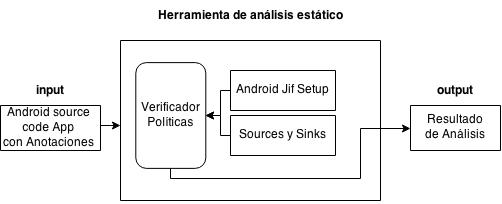
\includegraphics[width=10cm]{desing3-integration.jpg} 
% 	\end{center}
% 	\caption{Herramienta de análisis estático  }
% 	\label{fig:desingInteger}
% \end{figure}

% \begin{figure}[t!]
% 	\begin{center}
% 	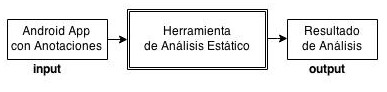
\includegraphics[width=9cm]{desingInOut-3.jpg}
% 	\end{center}
% 	\caption{Herramienta de análisis estático. Ilustra entradas y salidas
% 	esperadas}
% 	\label{fig:desing1}
% \end{figure} 

%color-question para Martín
% \textcolor{blue}{ \textit{P: desde este parrafo hasta el final de la sección,
% está bien dejar esa información así, o sencillamente la podemos omitir?}}\newline
% Luego, la estrategia de evaluación, consiste en verificar si la herramienta
% identifica pérdida de información mediante detección de flujos implícitos. Esto
% debido a que, como se menciona en la descripción del problema, parte importante
% de las propuestas para detección de fuga de información en aplicaciones Android,
% hacen data-flow analysis aplicando técnicas de análisis tainting, y en contraste
% con las técnicas de análisis de flujo de información, las técnicas de análisis
% tainting no necesariamente consideran flujos implícitos. Por tanto, al estar
% basada en JIF, cuyo enfoque de análisis es precisamente flujo de información, se
% esperaría que la herramienta propuesta esté en capacidad de reconocer flujos
% implícitos.
% 
% % Se esperaría que: al realizar análisis de flujo de información aplicando
% % técnicas Security-Typing, la herramienta propuesta, esté en capacidad de
% % reconocer flujos implícitos.\newline
% % Más específicamente, se puede tomar el conjunto de aplicaciones utilizadas como
% % casos de prueba para la detección de flujos implícitos en
% % DroidBench\cite{DroidBenchBenchmarks}, el benchmark de Flowdroid, y analizarlas
% % con la herramienta propuesta.\newline
% 
% Más específicamente, se puede partir de DroidBench\cite{DroidBenchBenchmarks},
% el benchmark de Flowdroid[\ref{FlowDroid-Tool}], tomar el conjunto de
% aplicaciones con que prueban la detección de flujos implícitos, y analizarlas
% con la herramienta propuesta.\newline
% Finalmente estos resultados serían
% comparados con los obtenidos mediante otras herramientas para análisis de fuga
% de información en aplicaciones Android.
% 
% En este orden de ideas, la evaluación de la herramienta propuesta está enfocada
% en: medir recall frente a la detección de flujos implícitos, es decir, medir que
% no genere falsos negativos ante la existencia de fugas de información,
% provenientes de flujos implícitos.\newline
% 
% 






\section{Limitaciones técnicas}
\label{sec:limitaciones}
Como parte del diseño de la solución, se inicia con una etapa exploratoria. En
esta se anotan manualmente varias aplicaciones de Android, y se identifican
limitaciones del lenguaje Jif para anotar código de la API de Android.
Tales limitaciones son adicionales a las características del lenguaje Java no
reconocidas por Jif, a continuación se describen tanto las encontradas, como las
especificadas en el manual de referencia de Jif.

-\textit{Características del lenguaje Java no soportadas por jif}\newline
Si bien, el sistema de anotaciones de Jif hace extensiones al lenguaje java,
permitiendo la evaluación de políticas de confidencialidad e integridad para
aplicativos implementados en dicho lenguaje, el manual de referencia de Jif
precisa las características del lenguaje Java no soportadas\cite{jifRef}. Estas
son:
\begin{itemize}
  \item nested classes: clases que son definidas dentro de otras clases.
  \item initializer blocks: bloques de código declarados dentro de la clase pero
  sin pertenecer a ningún método, dependiendo de si se trata de static
  initialization blocks, su código es el primero en ejecutarse, una vez se
  carga la clase; o si se trata de instance initialization blocks, su código se
  ejecutan cada vez que se crea una instancia de la clase.
\item threads.
\end{itemize} 
Partiendo de estas precisiones, aplicaciones Android que presenten tales
características son excluidas del grupo de aplicaciones a analizar(conjunto de
aplicaciones evaluables) mediante la herramienta propuesta.

% Adicional a las limitaciones de jif frente a características propias del
% lenguaje Java, tras experimentar la anotación manual de una serie de
% aplicaciones Android, se identifican varias limitaciones técnicas para la
% anotación de de las mismas. Entre las limitaciones identificadas están:\newline 

- \textit{Soporte para sobreescritura de métodos}\newline 
En la construcción de aplicaciones Android, según el componente que se esté
implementando(activities, content providers, receivers, services), se requiere
sobreescribir métodos de la clase que extienda el componente. Así, cuando se
define un componente tipo Activity, que debe extender de la clase Activiy.java, 
se sobreescriben métodos como Oncreate. Cada que se sobreescribe
un método se utiliza el statement @Override, con el cual se informa al
compilador de Java que el método es sobreescrito. No obstante, al implementar la
versión Jif de aplicaciones Android con dicho statement, el compilador de Jif
no lo reconoce. La dificultad que se presenta está en el reconocimiento del
statement(carácter @ y clase Override), y no en la sobreescritura de métodos,
puesto que Jif soporta tal característica. El soporte para la sobreescritura de
métodos es confirmado con una sencilla prueba, anotando la clase Activity.java
del framework Android (con un único método, el método Ocreate), e implementando
la versión Jif de una aplicación Android que extiende de tal clase, en la cual
se define una actividad y sobreescribe el método Oncreate.
Cuando se comenta la sentencia @Override, el compilador de Jif identifica la
sobreescritura del método y reporta comentarios para el flujo de información.\newline 
Al investigar el por qué Jif no reconoce tal sentencia, se encuentra que dentro
de las clases Java estándar soportadas por el compilador de Jif, no está
contenida la clase java.lang.Override.\newline
Las clases Java estándar pertenecientes a los paquetes io, lang, math, net y
sql; para las que el compilador Jif brinda soporte, vienen implementadas con
anotaciones en el directorio sig-src, directorio que forma parte de la
distribución del compilador de Jif con que se esté trabajando.\newline
Una alternativa para permitir el análisis de flujo de información entre métodos
que se sobreescriben, es comentar las líneas del programa que contengan la
sentencia @Override, puesto que, al no ser reconocida por el compilador de Jif,
es la generadora de errores de compilación.

- \textit{Casting entre tipos EditText y View}\newline
El framework de Android cuenta con diferentes clases para manejar las interfaces
gráficas que presenta al usuario, entre las cuales se encuentran EditText y
View. View es la clase principal para la creación de widgets, necesarios para la
implementación de componentes interactivos en las interfaces de usuario(UI).
EditText permite adicionar campos de texto editables en UI. El casting entre los
tipos de datos que representan ambas clases, se hace cuando la aplicación debe
procesar datos provenientes de campos en las interfaces del usuario, por ejemplo
como se observa a continuación:
\begin{lstlisting}
EditText editPassword = (EditText)findViewById(R.id.password);
String password = editPassword.getText().toString();
\end{lstlisting}
la interfaz de usuario(que es de tipo View) contiene un campo R.id.password, y
para manipular la información que almacena, debe ser de tipo EditText, siendo
necesario un casting de tipo View a tipo EditText. La dificultad que se presenta
con este tipo de casting es que para el sistema de anotaciones de jif no es
válido. Luego de probar con la anotación manual de ambas clases, tratando de
dar soporte a este tipo de casting, sin obtener resultados satisfactorios, se
opta por ``simular'' estos casos, es decir, si el tipo de dato de una variable
es de tipo EditText, se crea una variable tipo String con un valor determinado,
así se omite el casting y se puede analizar el flujo de información.

- \textit{Clase nested R}\newline
El framework de Android utiliza identificadores para hacer referencia a recursos
utilizados por la aplicación, recursos como strings, widgets y layouts, tales
identificadores son autogenerados en la clase R.java, allí cada recurso es
descrito como una clase individual. Al tratarse de una clase nested, la clase R
no puede ser anotada con jif. Esto puede solucionarse implementando una
versión Jif generalizada de la clase R, que contenga los recursos utilizados en
una aplicación, definidos como variables y no como clases.

% - \textit{Sources y Sinks}\newline
% En los preliminares para el diseño de la solución se propone utilizar SuSi
% para clasificar los sources y sinks en las aplicaciones a analizar, sin embargo, partir del
% extenso conjunto de sources y sinks, clasificados por SuSi para la API de
% Android, implica una mayor complejidad en el análisis, puesto que, en un
% aplicativo todo el código que le conforma puede hacer parte de sources o de
% sinks. Adicional a lo complejo que se puede tornar el análisis, los sources y
% sinks a considerar deben depender de la política de seguridad a evaluar. En ese
% orden de ideas, resulta más viable tomar un subconjunto del listado proveído por
% SuSi, partiendo de los sources y sinks que evalué la política de seguridad que
% se defina.

- \textit{Enhanced for loop} \newline
Además de soportar la estructura de control for, el lenguaje Java permite el uso
de enhanced for, que es utilizado para simplificar la iteración en arrays y
colecciones, por ejemplo:
% \begin{lstlisting}
% char c[] = imei.toCharArray();
% for (int i = 0; i < c.length; i++) {
% 	obfuscated += c[i] + "_";
% }          
% \end{lstlisting}  
\begin{lstlisting}
for(char c : imei.toCharArray())
obfuscated += c + "_";
\end{lstlisting}
A diferencia de Java, Jif no soporta el enhanced for.\newline
Debido a que ambas sentencias de control son equivalentes, la solución que se
propone para poder analizar flujo de información en los aplicativos Android que
contengan dicha estructura de control, es generar el equivalente del programa
haciendo uso del for, de este modo se cambia la sintaxis sin afectar la lógica
del aplicativo a analizar.

- \textit{Otras limitaciones} \newline
Adicional a las limitaciones descritas anteriormente, para las cuales se propone
una solución, se identifica que Jif no soporta la sintaxis utilizada para
definir estructuras de datos HashMaps, LinkedList y Sets, que en Java se definen
de la siguiente manera:
\begin{lstlisting}
Map<String,String> hashMap = new HashMap<String, String>();
List<String> listData;
Set<String> phoneNumbers = new HashSet<String>();
\end{lstlisting}
Jif tampoco permite la definición de interfaces como argumentos de un método. El
siguiente fragmento de código  en una aplicación Android, muestra la definición
de una interfaz pasada como parámetro al método setOnClickListener.
\begin{lstlisting}
   Button button1= (Button) findViewById(R.id.button1);
   button1.setOnClickListener(new View.OnClickListener() {
   ...
   .....}  });
\end{lstlisting}
En estos casos, la dificultad está en encontrar una sintaxis que permita obtener
la versión equivalente del programa que las contenga. A lo que se suma, la falta
de documentación disponible para solventar los mismos. En consecuencia, se omite
del conjunto de aplicaciones evaluables, aplicaciones Android que requieran en
su implementación las estructuras de datos descritas.\newline

%- \textit{Paso de statements dentro de los argumentos de un método
%(\{\}):}\newline

\section{Diseño de la solución}
Como se describe en la propuesta de solución \ref{sec:propuesta-sol}, el
diseño ideal para contribuir con la solución del problema es: una herramienta
que contenga el setup de Jif para Android, e integregre un clasificador de
sources y sinks, de tal manera que la herramienta permita evaluar el control de
flujo de información en aplicativos Android. Así, mediante anotaciones Jif en el
código de su aplicación, el desarrollador define la política de seguridad a evaluar.

Sin embargo, para efectos de esta tesis se limitia el Setup de Jif, partiendo de
una política de seguridad específica. De este modo, el diseño se centra en
soportar un conjunto reducido de clases de la Api de Android, y en incluir un
conjunto específico de sources y sinks de acuerdo a una política de seguridad
establecida. Ese conjunto de sources y sinks, se toma del listado de sources y
sinks proveido por SuSi \ref{sec:susi}.\newline 
Adicionalmente para aspectos de evaluación, se incluye el diseño de un anotador
que anota automáticamente el conjunto de aplicativos a analizar acorde a la
política de seguridad que se evalua. La figura \ref{fig:desingReal} muestra el
esquema del diseño.
\begin{figure}[t!]
	\begin{center} 
	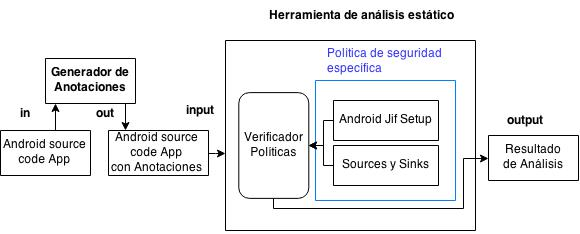
\includegraphics[width=11cm]{desing3Real.jpg} 
	\end{center}
	\caption{Diseño herramienta de análisis estático}
	\label{fig:desingReal}
\end{figure}

% En los preliminares para el diseño de la solución se consideró la siguiente
% opción: Anotar un conjunto de clases de la API de Android mediante el sistema de
% anotaciones de Jif, de modo que el compilador de Jif reconociera clases propias
% de esa API, y por tanto, permitiese el análisis de flujo de información a través
% de estas. Habiendo asegurado el reconocimiento a un
% conjunto de clases de la API de Android, era tarea del desarrollador implementar
% la versión Jif del aplicativo a evaluar.
% 
% Si bien, con dicha opción de diseño se aporta para que el desarrollador
% Android evalúe flujos de información en su aplicación, mediante Jif; también se
% incrementa su carga de programación, puesto que, al delegarle la anotación de la
% aplicación a analizar, este debe pensar dos versiones. La versión .java, donde
% utiliza los métodos proveídos por la API Android para definir las
% funcionalidades de su aplicación; y la versión .jif, donde define las
% anotaciones pertinentes para evaluar flujos de información; tarea para la cual,
% se requiere un conocimiento previo del sistema de anotaciones de Jif y la
% implementación de aplicaciones haciendo uso de las mismas.
% 
% En consecuencia, se opta por un diseño que reduzca la carga de programación
% del desarrollador, durante el análisis del aplicativo.\newline 
% El diseño de solución consta de dos elementos fundamentales: anotaciones a la
% API de Android, más el anotador que genere la versión Jif del aplicativo a
% analizar, acorde a una política de seguridad previamente definida.\newline 
% Ambos elementos son complementarios, puesto que, por más que se genere la
% versión Jif del aplicativo a analizar, si el compilador no reconoce clases
% específicas de la API que allí se usan, .jif no puede ser compilado.

Así, (1) se parte definiendo la política de seguridad a evaluar
\ref{subsection:politica}, (2) se toman a consideración elementos influyentes
para verificar el cumplimiento de la política mediante Jif
\ref{subsec:consVerPol}, y finalmente, teniendo en cuenta (1) y (2), se definen
los lineamientos de anotación \ref{subsec:linemientos}, donde se define el
esquema de anotación tanto para las anotaciones requeridas en la API como para
las anotaciones de los aplicativos a analizar(linemientos del anotador).

\subsection{Definición de la política de seguridad}
\label{subsection:politica}
Detectar si una aplicación Android(perteneciente al conjunto evaluable) presenta
flujos de información entre, información con nivel de seguridad alto e
información con nivel de seguridad bajo.\newline
Detectando fugas de información catalogada con nivel de seguridad alto, vía:
canales creados durante el control de flujo del programa(flujos implícitos),
mensajes de texto y mensajes de Log.\newline 

\subsection{Consideraciones para verificar el cumplimiento de la política
mediante Jif} 
\label{subsec:consVerPol}
Teniendo definida la política de seguridad a verificar, se describen
elementos influyentes en el diseño de la solución.

\textit{Información considerada con nivel de seguridad alto}\newline
Para verificar el cumplimiento de la política de seguridad a evaluar se parte de
un conjunto de sources(), caracterizados por dar a conocer información del
usuario, considerada como privada o sensible. Los métodos que integran
el conjunto de sources son: getDeviceId, getSimSerialNumber, findViewById,
getLatitude, getLongitude y getSubscriberId. Adicional a estos métodos, se
incluye el tipo de dato EditText, si y sólo si, el campo UI al que referencia
corresponde a un campo tipo textPassword, es decir, un campo que almacena
contraseñas.\newline 

\textit{Canales que muestran información con nivel de seguridad bajo}\newline
La información enviada a través de mensajes de texto y la información conocida
tanto a través de mensajes de Log, como a través de canales generados por el
control de flujo del programa, tiene en común que debe poder ser conocida por
terceros. En consecuencia, se considera que estos canales deben dar a conocer
información con nivel de seguridad bajo.\newline
En el caso de mensajes de texto y mensajes de Log, se hace referencia
específicamente a las clases Log y SmsManager de la API de Android.

\textit{Diferencia entre una aplicación Android y una aplicación Java
convencional}\newline 
En esencia, una aplicación Android es una aplicación Java con interfaces
descritas en XML, que para ser ejecutada necesita del framework de Android,
porque este le provee acceso al hardware del dispositivo y funcionalidades del
sistema.\newline 
Por otro lado, Jif permite hacer seguimiento al flujo de información de una
aplicación Java, extendiendo el lenguaje mediante labels de seguridad.\newline
Para analizar flujo de información de una aplicación Android mediante
Jif, es importante mencionar que mientras una aplicación Java convencional
cuenta con un único punto de entrada para iniciar su ejecución, esto es, la
clase principal donde se implementa el método main; una aplicación Android puede
tener más de un punto de entrada, generados a partir de los diferentes tipos de
componentes que le integren(Activity, Service, Content Provider y Broadcast
Receiver). La necesidad de interacción del usuario para activar tales puntos de
entrada varía acorde al tipo de componente, así, en el caso de componentes tipo
Activity su ejecución sólo inicia hasta que el usuario interactúe con la
actividad, y para manejar dicha interacción, la API Android provee el método
OnCreate. De otro modo, componentes tipo Service y Broadcast Receiver, inician
su ejecución a través de los métodos OnStartCommand y OnReceive,
respectivamente, sin necesidad de interacción del usuario.\newline 
{ \color{black} {Teniendo en cuenta lo anterior, se asume que la aplicación a
evaluar tiene un único punto de entrada, que depende del tipo de componente que
implemente.} }

\textit{Chequeo de excepciones tipo Runtime}\newline
En lenguaje Java las excepciones tipo Runtime tales como NullPointerException, no
son verificadas a tiempo de compilación, sin embargo, buscando evitar la
generación de canales encubiertos mediante las mismas, Jif si las verifica. 
En consecuencia, si un programa requiere excepciones NullPointerException,
ClassCastException y/o ArrayIndexOutOfBoundsException, el programador debe
declararlas en el programa, de lo contrario, el compilador de Jif genera error.
Para las aplicaciones a analizar, se espera que el desarrollador haya
especificado las excepciones necesarias.

\textit{Evaluación del flujo de información}\newline
Para evaluar el flujo de información, se asume que todos los métodos definidos
en la clase serán invocados, y por tanto, todos son incluidos en el análisis.\newline 
Esta decisión de análisis busca evitar el paso inadvertido de flujos de
información, generados por omisión.

\textit{Acceso a métodos de sobreescritura.}\newline
Los métodos de las clases Activity, Service y BroadcastReceiver, son métodos
que se pueden sobreescribir, todo programa Android que extienda de tales clases
debe poder utilizarlos.

\subsection{Lineamientos de anotación}
\label{subsec:linemientos}
Para verificar el cumplimiento de la política de seguridad
establecida \ref{subsection:politica} mediante el sistema de anotaciones de Jif,
se requiere: (a) definir los elementos básicos de anotación, (b) definir
las anotaciones necesarias para la API de Android y (c) definir los
criterios de anotación para los aplicativos a analizar, tales 
criterios se sintetizan en un anotador.

%\textbf{(a)Elementos básicos de anotación}\newline
\subsubsection{Elementos básicos de anotación}
En \ref{subsec:consVerPol} se definió qué \textit{Canales muestran
información con nivel de seguridad bajo} y cuál es la \textit{Información
considerada con nivel de seguridad alto}. Ahora, para anotar la información
catalogada con uno u otro nivel de seguridad, de modo que, partiendo de tales
anotaciones se evalué la existencia de flujos de información entre información
con nivel de seguridad alto e información con nivel de seguridad bajo, lo primero
que se debe definir es quién es la autoridad de los programas y cuáles son los
labels de seguridad.\newline
Conceptos y términos implicados en la sintaxis de anotación Jif, se
encuentran en la sección de background \ref{sssec:JifSintax}.

Principal \emph{Alice}\newline
aprovechando que Jif ya trae una serie de principals establecidos, se define que
la autoridad máxima es el principal Alice. Este principal tendrá todo el poder
para actuar sobre aspectos de los programas.

Label de seguridad \emph{\{Alice:\}}\newline
este label indica que la información tiene nivel seguridad alto, es decir, que
se trata de información sensible o privada.\\
Variables con nivel de seguridad alto deben ser anotadas con tal label de
seguridad, porque esté epecífica que sólo el dueño de la información(Alice)
puede acceder a la misma. 

Label de seguridad \emph{\{\}}\newline
este label indica que la información tiene nivel de seguridad bajo, es decir,
información de conocimiento público.

\subsubsection{Anotaciones a la API de Android}
%\textbf{(b)Anotaciones a la API de Android}\newline

\begin{figure}[h!]
	\begin{center}
	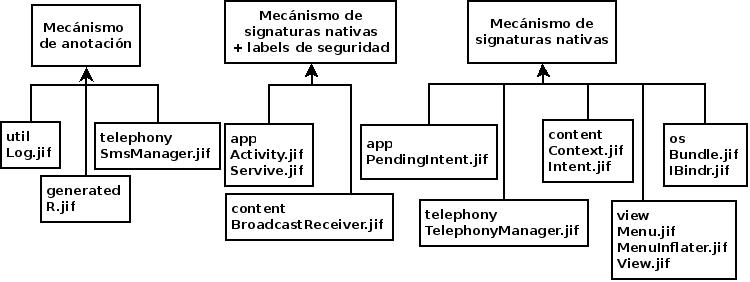
\includegraphics[width=12cm]{annotationsMechanims.jpeg}
	\end{center}
	\caption{Mecánismos de anotación para clases de la API.}
	\label{fig:annotationsMechanims}
\end{figure}

- Anotaciones para \textit{Canales que muestran información con nivel de
seguridad bajo}: para controlar el flujo de información que se envía hacia
\textit{Canales que muestran información con nivel de seguridad bajo}, es
necesario anotar la definición de los métodos de las clases Log y SmsManager de
la API Android, de manera tal, que se controle el nivel de seguridad de los
argumentos con que se invocan.\newline
Tomando como ejemplo el método sendTextMessage de la clase SmsManager, mediante
el cual se envían mensajes de texto:\newline
public final void sendTextMessage (String destinationAddress, String
scAddress, String text, PendingIntent sentIntent, PendingIntent
deliveryIntent)\newline
El argumento \emph{text} es el que recibe la información a mostrar, por tanto
esa información debe ser pública.\newline 
Por consiguiente, en la definición del método el label de seguridad del
argumento(AL) correspondiente a la información a mostrar(logs) o la información
a enviar(sms), se anota con el label de seguridad bajo(label público\{\}). Con
esto se garantiza que la información se muestra o envía, si y sólo si el nivel
de seguridad del argumento con que se invoca el método es público. Por ejemplo,
si el método se llama con información anotada con label de seguridad alto, se
genera error en la compilación del programa que le llama.\newline 
El resto de argumentos del método se anotan con label de seguridad \{Alice:\},
puesto que esa información puede ser pública o privada.\newline
En el caso del BL al anotarlo con el label \{Alice:\}, se permite que el método
sea invocado desde cualquier punto de un programa. 
Para el resto de labels se dejan los que Jif genera por defecto\newline
% cualquier punto de un programa que sea igual o menor de restrictivo que el
% principal Alice, esto se traduce en que podrá ser invocado desde cualquier punto
% de un programa, lo cual es correcto porque lo que se busca el evitar que se
% envíe información considerada con nivel se deguridad alto y no, evitar que el
% método sea utilizado. Poner ejemplo XXXX?\newlie
- Anotaciones para metódos de sobreescritura: en \ref{subsec:consVerPol},
también se definieron las clases de la API para las que se debe soportar el
\textit{Acceso a métodos de sobreescritura}(Activity, Service y
BroadcastReceiver). La anotación para la definicíon de tales métodos se basa en:
(1)reglas de Jif para la sobreescritura de métodos y (2)desde dónde pueden ser
invocados. (1)Jif exige que el nivel de seguridad del BL del método desde donde
se invoca el método a sobreescribir, no debe ser menos restrictivo que el BL de
la definición de tal método(privado es más restrictivo que público). (2) la
sobreescritura de métodos se debe poder utilizar desde aplicativos que extiendan
de las clases Activity, Service y BroadcastReceiver.\newline 
Para cumplir con (1) y (2), los métodos que requieren ser sobreescritos se
definen con BL público(\{\}). De este modo los aplicativos desde dónde se
invocan los métodos a sobreescribir deben tener igual BL.

- Adicional a las clases de la API (Log, SmsManager, Activity, Service y
BroadcastReceiver), es necesario brindar soporte a un conjunto de clases que
representan librerias importadas por los aplicativos a analizar.(Estas
son)Brindar soporte significa que deben ser reconocidas por el compilador Jif.

% Y para poder integrarlas al conjunto de clases reconocidas por el compilador
% de Jif, basta con recurrir a signaturas nativas. Mediante el uso de signaturas
% nativas es posible incluir clases Java ya existentes. Tal mecanismo consiste en
% implementa una versión Jif de las clase fuentes, en la qué sólo es necesario
% declarar constructores y cuerpo de los métodos a utilizar.
% 
% Ahora, para incluir clases Java ya existentes es posible recurrir a signaturas
% nativas, con las cuales se implementa la versión Jif de las clases fuentes, esto
% es, declarando constructores y cuerpo de los métodos a utilizar.
- Integración de clases de la API de Android a las clases reconocidas por el
compilador de Jif:\newline
Definidos los criterios de anotación para las clases de la API, a las cuales se
debe implementar su respectiva versión Jif. Se definen los mécanismos a utilizar
para implementar tal versión. Además del mecanismo de anotación completa en que
se basa la implementación de aplicativos en Jif(mecanismo de anotación), el
compilador provee un mecanismo que permite reutilizar código de clases Java ya
existentes, para esto, se recurre a signaturas nativas. Así, se implementa una
versión Jif de una clase Java ya existente, en la que se declaran signaturas
nativas proveídas por Jif, constructor y métodos necesarios de la
clase(mecanismo de signaturas nativas).
Dependiendo de las implicaciones que pueda tener para el análisis de flujo de información del
sistema, a la versión simplificada puede específicar u omitir labels de
seguridad(mecanismo de signaturas nativas más labels de seguridad).\newline 
Para el presente caso y de acuerdo a los criterios de anotación previamente
establecidos las clases a implementar mediante uno u otro mecanismo, son
ilustrados en la siguiente figura \ref{fig:annotationsMechanims}.\newline

\subsubsection{Anotaciones en los aplicativos a analizar}
%\subsubsection{Criterios de anotación para los aplicativos a analizar}
%\textbf{(c)Criterios de anotación para los aplicativos a analizar}\newline
% XXXPara evaluar los flujos de información de una aplicación Android, de modo que
% se verifique si cumplen con la política de seguridad definida
% \ref{subsection:politica}; es necesario implementar su respectiva versión Jif,
% esto implica que variables y métodos de la clase sean anotados haciendo uso del
% sistema de anotaciones de Jif.\newline 
% Ante esto, se propone un esquema de anotación enfocado a detectar flujos de
% información desde: información considerada con nivel de seguridad alto,
% hacia: canales considerados con nivel de seguridad bajoXXX.
Los elementos en que se fundamenta el esquema de anotación para el aplicativo a
analizar, son los siguientes:\newline 
Primero, como los \textit{Canales que muestran
información con nivel de seguridad bajo} están anotados desde la definición en
sus respectivas clases de la API, de modo que la información a mostrar(logs) o
enviar(msn) debe tener nivel de seguridad bajo(debe ser pública), en el esquema
de anotación del aplicativo no es necesario identificar tales canales, pues
estos ya están definidos desde la API. Lo que si se debe hacer desde el esquema
de anotación del aplicativo, es proveer los labels de seguridad adecuados a la
información con que se invocan tales canales.

Segundo, la anotación para la sobreescritura de métodos de la API, está definida
en las respectivas clases de la API, el esquema de anotación para la invocación
de los métodos a sobreescribir debe ser consecuentes con tales definiciones de
anotación.

Tercero, el esquema de anotación para el aplicativo a analizar parte de
los sources que se identifiquen en el mismo. Tales sources pertenecen al conjunto
definido en (\textit{Información considerada con nivel de seguridad alto}),
conjunto que está integrado por el tipo de dato EditText\footnote{Este tipo de
dato es considerado como source si y sólo si, el campo UI al que referencia
corresponde a un campo tipo textPassword, es decir, un campo que almacena
contraseñas.} y los métodos: getDeviceId, getSimSerialNumber, findViewById,
getLatitude, getLongitude y getSubscriberId.

Cuarto, se parte de los \textit{Elementos básicos de anotación} prevíamente
definidos. Así, una clase Android tendrá como principal( autoridad máxima) al
principal \emph{Alice}, y los labels de seguridad para anotar información con
nivel de seguridad alto y nivel de seguridad bajo son: \emph{\{Alice:\}} y
\emph{\{\}}, respectivamente.

\textbf{\textit{Estructuración del esquema de anotación}}\newline 
Para concretar el esquema con que se anotan los aplicativos a analizar, se
establece la finalidad(Objetivo de la anotación), qué se va a anotar(Elementos
del esquema), cómo se van a anotar tales elementos(Anotación de los elementos) y
finalmente se indica cómo aplicar el esquema de anotación(Pasos para aplicar el
esquema de anotación). Así:

\textit{Objetivo de la anotación}\newline
El esquema de anotación se centra en identificar si una clase contiene sources,
y verificar si los métodos de la clase influencian esa información, de modo que,
cuando la información sea envíada por canales con nivel de seguridad bajo, tenga
el nivel de seguridad adecuado.

\textit{Elementos del esquema}\newline
Para referenciar los elementos que se anotan mediante este esquema, se
establecen una serie de términos, así:\newline
- Variable source: una variable source es una variable que almacena
información proveída por algún elemento del conjunto de sources.\\
- Array source: un array source es un array que almacena información de
variables source.\\
- Método que se sobreescribe: hace referencia a métodos de la API android
que deben ser sobreescrtos para la implementación del aplicativo, por ejemplo, el
método Oncreate que se sobreescribe al implementar componentes tipo
Activity.\\
- Método source: un método source es un método(definido dentro de la
clase) que cuando es invocado, contiene dentro de los parámetros de invocación, al menos
una varible source.\\
- Método no source: un método no source es un método(definido dentro de la
clase) que cuando es invocado, no contiene dentro de los parámetros de invocación,
varibles source.

\textit{Anotación de los elementos}\newline
Fijados los elementos que se anotan, se define su respectiva forma de anotación.
Conceptos y términos implicados en la sintaxis de anotación Jif, se
encuentran en la sección de background \ref{sssec:JifSintax}.
Los labels de seguridad que no son anotadas mediante este esquema, son generados
automáticamente por Jif, acorde a los labels que estable por defecto para la
definición de variables, métodos y arrays, etc.

- Definición A: anotación de variable source.\newline 
\emph{java-type \{Alice:\} nameVar}\newline
como la información almacenada en una variable source es información con nivel
de seguridad alto(conjunto de sources), la variable debe tener un label de
seguridad que indique que su información es de alta confidencialidad. Al
anotarla con el label \emph{\{Alice:\}}, se está indicando que esa información
pertenece al principal \emph{Alice}, así, cuando se envíe hacia un canal
de seguridad bajo, da lugar a un flujo de información indebido(de nivel alto a
nivel bajo).

- Definición B: anotación de array source.\newline
\emph{java-type\{Alice:\}[ ]\{Alice:\} arrayName}\newline
debido a que un array source almacena información con nivel de seguridad alto,
se debe garantizar que sólo el principal dueño de la información pueda
conocer tanto items como tamaño del array. Esto se logra anotando con
label de seguridad \emph{\{Alice:\}} el \emph{BL} y \emph{SL}, labels de
seguridad para los elementos y tamaño del array, respectivamente.

- Definición C: anotación de método que se sobreescribe.\newline
El BL de un método a sobreescribir debe ser anotado con label de seguridad bajo
\{\}, puesto que en su respectiva definición en las clases de la API, han sido
definidas con ese BL.

- Definición D: anotación de método source.\newline 
\emph{java-type\{Alice:\}  methodName \{Alice:\}(java-type arg1\{Alice:\} ,,,
java-type argn\{Alice:\})}
Como un método source influencia información con nivel de seguridad alto(variable
source), se debe garantizar que sólo sentencias del programa que tengan nivel de
seguridad alto, puedan ser actualizadas con información proporcionada por el método.\\
Buscando hacer cumplir lo anterior, se anota con label de
seguridad \{Alice:\} el RTL y el BL del método.
Retomando la sintaxis jif para anotación de métodos:\newline 
\emph{java-type \{RTL\} methodName \{BL\} (java-type arg1\{AL\},,, java-type argn\{AL\}):\{EL\} }\newline
Al anotar \{RTL\} con \{Alice:\} se asegura que, si el método retorna un valor,
tendrá nivel de seguridad alto.\newline
Al anotar \{BL\} con \{Alice:\} se asegura que, los puntos del programa que
traten de ser actualizados tras el llamado del método(por ejemplo variables, o
resultados de condicionales) deben tener un \underline{pc} con nivel de
seguridad alto.\newline
Para el caso de los AL, labels de seguridad de los argumentos, el sistema de
anotaciones de Jif exige que los AL con que se invoca el método, deben ser igual
o menor de restrictivos que los AL con que se define el método. 
Por otro lado, se tiene certeza de que uno de los argumentos con que se llama el
método tiene AL con nivel de seguridad alto(pues ese fue el criterio con que
se clasificó al método como source), pero el resto de párametros puede tener AL
alto o bajo, entonces para garantizar que el método pueda ser invocado bajo
tales condiciones, los AL para los argumentos del método son anotados con
label \{Alice:\}.

- Definición E: anotación de método no source.\newline
\emph{methodName \{\} (java-type arg1\{Alice:\},,, java-type argn\{Alice:\})}\newline
Como el método no recibe la variable source, el nivel de seguridad de las
sentencias del programa que se actualicen con la información del método puede
ser bajo. Ahora,  si en el cuerpo del método se define o actualiza información
con nivel de seguridad alto(información global), tales sentencias deben tener
nivel de seguridad alto.
Anotando el BL con label {\{\}}, se respeta tal condición puesto que,
el BL se ve afectado cuando el cuerpo del método tiene información con mayor
nivel de seguridad, obligando a que las sentencias a actualizarse con la
información del método tengan nivel de seguridad alto.\newline
Para el caso de los AL, labels de seguridad de los argumentos, el sistema de
anotaciones de Jif exige que los AL con que se invoca el método, deben ser igual
o menor de restrictivos que los AL con que se define el método. Anotando los AL
de la definición del método con label \{Alice:\}, se cumple tal restricción ya
que el método es invocado con parámetros cuyo nivel de seguridad es bajo.

\textit{Pasos para aplicar el esquema de anotación}\newline
Partiendo de las anteriores definiciones, los pasos para la anotación son los
siguientes:\newline
(1) Identificar variables source de la clase. Si se encuentran variables sources
continuar con los pasos (2) a (11), sino, continuar con pasos: (3), (6), (9) y
Aplicar Definición E a los métodos que no se sobreescriben\footnote{Como no se
identifican sources, la anotación de método no source(Definición E) es
aplicable para los métodos que no se sobreescriben.}.
(2) Identificar arrays sources de la clase.
(3) Identificar el total de métodos de la clase.\newline
(4) Del total de métodos listar los métodos source.\newline
(5) Del total de métodos listar los métodos no source.\newline
(6) Del total de métodos listar los métodos a sobreescribir\newline
(7) Aplicar Definición D a listado del paso(4).\newline
(8) Aplicar Definición E a listado del paso (5).\newline
(9) Aplicar Definición C a listado del paso (6).\newline
(10) Aplicar Definición B a listado del paso (2).\newline
(11) Aplicar Definición A a listado del paso (1).

Para automatizar estos pasos, se debe implementar un generador de
anotaciones(prototipo de anotación). Que reciba como entrada el código fuente de
la aplicación Android(perteneciente al conjunto evaluable), y retorne su
respectiva implementación en Jif, versión que contiene las anotaciones para
evaluar la política de seguridad definida.\newline
La figura \ref{fig:desingSolution}, ilustra las entradas y salidas
esperadas.\newline
Luego la versión obtenida se evalúa con el compilador de Jif.
% \textit{Entradas y salidas del anotador}.
% Las definiciones y pasos para la anotación del aplicativo a analizar, descritas
% anteriormente, se condensan en un anotador. El cual debe recibir como entrada el
% código fuente de la aplicación Android(perteneciente al conjunto evaluable),
% para retornar su respectiva implementación en Jif, versión que contiene las
% anotaciones para evaluar la política de seguridad definida. Tal como se ilustra
% en la figura \ref{fig:desingSolution}\newline 
% Luego la versión obtenida se evalúa con el compilador de Jif.
\label{subsec:anotador}
\label{subsec:pasosSol}
\begin{figure}[t!]
	\begin{center}
	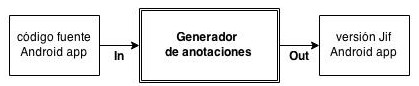
\includegraphics[width=10cm]{desingSolution2.jpg}
	\end{center}
	\caption{Entradas y salidas para el generador de anotaciones.}
	\label{fig:desingSolution} 
\end{figure}

% \subsection{Anotaciones a la API de Android}
% \label{subsec:apiAnnotations}
% 
% \begin{figure}[h!]
% 	\begin{center}
% 	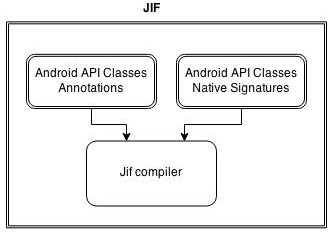
\includegraphics[width=5cm]{desingSol-steps1.jpg}
% 	\end{center}
% 	\caption{Tipos de anotación necesarias para implementar la solución.}
% 	\label{fig:desingSol-steps1}
% \end{figure}
% 
% \begin{figure}[t!]
% 	\begin{center}
% 	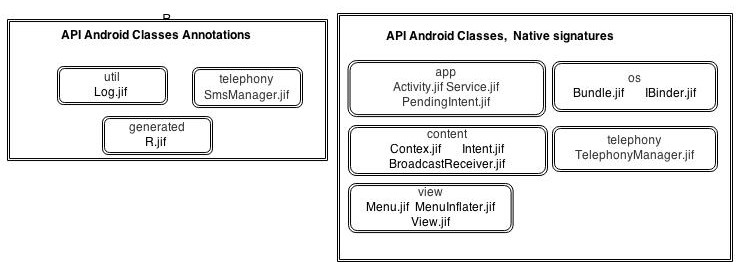
\includegraphics[width=12cm]{desingSol-step1-details.jpg}
% 	\end{center}
% 	\caption{Clases de la API a anotar.}
% 	\label{fig:desingSol-details}
% \end{figure}
% 
% El compilador de Jif tiene implementadas mediante el sistema de anotaciones Jif,
% las clases estándar del lenguaje Java para las que brinda soporte.\newline
% Ahora, para incluir clases Java ya existentes es posible recurrir a signaturas
% nativas, con las cuales se implementa la versión Jif de las clases fuentes, esto
% es, declarando constructores y cuerpo de los métodos a utilizar.
% 
% Para dar soporte a clases específicas de la API de Android se recurre a ambas
% opciones de anotación. Tal como se ilustra en la figura
% \ref{fig:desingSol-steps1}.\newline 
% El criterio para decidir que se anota de una u otra forma, depende de lo que
% represente la clase Android para verificar la política de seguridad
% establecida.\newline
% Las clases Log y SmsManager, que representan canales para conocer información,
% son anotadas de forma no nativa.\newline
% La opción de anotación nativa se utiliza
% para librerías Android, por ejemplo la clase TelephonyManager necesaria para utilizar
% el método getDeviceId.\newline
% En la figura \ref{fig:desingSol-details} se
% especifican clases de la API Android a anotar.\newline

\subsection{Descripción implementación}
Como se describio anteriormente, la implementación del diseño requiere
anotaciones a la API de Android y anotaciones en los aplicativos a
analizar.\newline 
En el caso de las anotaciones requeridas para la API, su
implementación se hace manualmente.\newline
En el caso de las anotaciones en el aplicativo a analizar, para lo
cual se propuso un esquema de anotación automatizable, se implementa un
prototipo de anotación en lenguaje Java. En la sección \ref{sec:diagramaClass}
de los anexos, se incluye su respectivo diagrama de clases.\newline
El anotador consta de cinco clases: Main, Source, XmlExtract, Annotation y
BufferWriter. 
En la clase Main se coordinan todos los pasos de anotación, así, la clase
Sources  identifica qué variable sources contiene la aplicación que se está
analizando; la clase Source  se apoya en la clase XmlExtract  para
identificar el source EdidText cuando el campo UI al que referencia corresponde
a un tipo textPassword. Como las interfaces UI se describen mediante XML, es
necesario extraer los datos de la interfaz con parsers XML.\\
Con la clase Annotation  se identifican y anotan los diferentes tipos de
métodos(métodos source, no source y métodos a sobreescribir).
En la clase BufferWriter  se anotan las variables sources, y finalmente se
retorna la versión .jif del aplicativo que se está analizando.\newline 
Para la anotación del código se utiliza la librería Java Parser 1.8  que permite
generar y visitar el arbol de sintaxis para la estructura del código de cada
programa, haciendo posible la adición de los labels de seguridad respectivos.\\
(Incluir Figura)\newline
\label{subsec:anotador}
\begin{figure}[t!]
	\begin{center}
	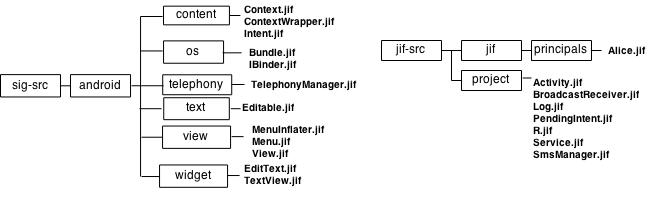
\includegraphics[width=12cm]{JifFilesystem.jpg}
	\end{center}
	\caption{Estructura de directorios en Jif.}
	\label{fig:jifFilesystem} 
\end{figure}

\subsection{Ambiente y herramientas}
\textit{Versión de la API de Android}\newline
Las anotaciones a las clases de la API Android y las aplicaciones a anotar
mediante el prototipo, corresponden a la versión Android 4.2.2(API Level 17).

\textit{Versión del compilador de Jif}\newline
El componente que verifica el cumplimiento de las políticas de seguridad,
corresponde a la versión 3.4.2 del compilador de Jif.

\textit{Estructura de trabajo en JIF}\newline
El compilador de Jif maneja una estructura de directorios en la que se incluye
el código fuente .jif de las aplicaciones a analizar. Como ilustra la figura
\ref{fig:jifFilesystem} se tienen los directorios principales sig-src y jif-src.
El directorio sig-src está destinado para incluir librerías adicionales.\newline 
El directorio jif-src contiene todo el código jif correspondiente al programa
como tal que se va evaluar mediante Jif. Para los propósitos del presente
trabajo, se tienen los subdirectorios principals y project. En el subdirectorio
principals se incluyen las autoridades requeridas, y en el subdirectorio
project se incluyen, tanto las clases específicas de los aplicativos Android a
analizar, como las clases de que estos heredan como: Activity.jif, Service.jif,
etc.

\subsection{Compilación, integración y finalmente ejecución }
En \ref{sec:ejecutarPrototipo} se describen las intrucciones paso a paso de cómo
ejecutar el anotador, y cómo compilar los aplicativos a analizar mediante Jif.






















% %\chapter{Descripción implementación}

\section{Limitaciones técnicas}
\label{sec:limitaciones-tec}
Antes de iniciar con la implementación del esquema de anotación propuesto, tanto
para las clases de la API \ref{subsec:api}, como para los aplicativos a analizar
\ref{subsec:apps}, se identifican una serie de limitaciones del lenguaje
Jif para anotar código de la API de Android. 
Tales limitaciones son adicionales a las características del lenguaje Java no
soportadas por Jif, a continuación se describen tanto las encontradas, como las
especificadas en el manual de referencia de Jif.

\subsection{Características del lenguaje Java no soportadas por jif}
% -\textit{Características del lenguaje Java no soportadas por jif}\newline
Si bien, el sistema de anotaciones de Jif hace extensiones al lenguaje java,
permitiendo la evaluación de políticas de confidencialidad e integridad para
aplicativos implementados en dicho lenguaje, el manual de referencia de Jif
precisa las características del lenguaje Java no soportadas\cite{jifRef}. Estas
son:
\begin{itemize}
  \item nested classes: clases que son definidas dentro de otras clases.
  \item initializer blocks: bloques de código declarados dentro de la clase pero
  sin pertenecer a ningún método, dependiendo de si se trata de static
  initialization blocks, su código es el primero en ejecutarse, una vez se
  carga la clase; o si se trata de instance initialization blocks, su código se
  ejecutan cada vez que se crea una instancia de la clase.
\item threads.
\end{itemize} 
Partiendo de estas precisiones, aplicaciones Android que presenten tales
características son excluidas del grupo de aplicaciones a analizar(conjunto de
aplicaciones evaluables) mediante la herramienta propuesta.

% Adicional a las limitaciones de jif frente a características propias del
% lenguaje Java, tras experimentar la anotación manual de una serie de
% aplicaciones Android, se identifican varias limitaciones técnicas para la
% anotación de de las mismas. Entre las limitaciones identificadas están:\newline 
\subsection{Soporte para la clase java.lang.Override}
\label{sub:override}
% - \textit{Soporte para sobreescritura de métodos}\newline 
En la construcción de aplicaciones Android, según el componente que se esté
implementando(activities, content providers, receivers, services), se requiere
sobreescribir métodos de la clase que extienda el componente. Así, cuando se
define un componente tipo Activity, que debe extender de la clase Activiy.java, 
se sobreescriben métodos como Oncreate. Cada que se sobreescribe
un método se utiliza el statement @Override, con el cual se informa al
compilador de Java que el método es sobreescrito. No obstante, al implementar la
versión Jif de aplicaciones Android con dicho statement, el compilador de Jif
no lo reconoce. La dificultad que se presenta está en el reconocimiento del
statement(carácter @ y clase Override), y no en la sobreescritura de métodos,
puesto que Jif soporta tal característica.\newline 
El soporte para la sobreescritura de
métodos es confirmado con una sencilla prueba, anotando la clase Activity.java
del framework Android (con un único método, el método Ocreate), e implementando
la versión Jif de una aplicación Android que extiende de tal clase, en la cual
se define una actividad y sobreescribe el método Oncreate.
Cuando se comenta la sentencia @Override, el compilador de Jif identifica la
sobreescritura del método y reporta comentarios para el flujo de información.

Al investigar el por qué Jif no reconoce tal sentencia, se encuentra que dentro
de las clases Java estándar soportadas por el compilador de Jif, no se incluye
la clase java.lang.Override.\newline 
Las clases Java estándar pertenecientes a los paquetes io, lang, math, net y
sql; soportadas po el compilador Jif, vienen implementadas con anotaciones en el
directorio sig-src, directorio que forma parte de la distribución del compilador
de Jif con que se esté trabajando.

Un mecanismo para permitir el análisis de flujo de información entre métodos
que se sobreescriben, es comentar las líneas del programa que contengan la
sentencia @Override, puesto que, al no ser reconocida por el compilador de Jif,
es la generadora de errores de compilación.

\subsection{Casting entre tipos EditText y View}
\label{sec:casting}
El framework de Android cuenta con diferentes clases para manejar las interfaces
gráficas que presenta al usuario, entre las cuales se encuentran EditText y
View.\newline
View es la clase principal para la creación de widgets, necesarios para la
implementación de componentes interactivos en las interfaces de
usuario(UI).\newline 
EditText permite adicionar campos de texto editables en UI.\newline
El casting entre los tipos de datos que representan ambas clases, se hace cuando la aplicación debe
procesar datos provenientes de campos en las interfaces del usuario, por ejemplo
como se observa a continuación:
\begin{lstlisting}
EditText editPassword = (EditText)findViewById(R.id.password);
String password = editPassword.getText().toString();
\end{lstlisting}
la interfaz de usuario(que es de tipo View) contiene un campo R.id.password, y
para manipular la información que almacena, debe ser de tipo EditText, siendo
necesario un casting de tipo View a tipo EditText. La dificultad que se presenta
con este tipo de casting es que para el sistema de anotaciones de jif no es
válido. Luego de probar con la anotación manual de ambas clases, tratando de
dar soporte a este tipo de casting, sin obtener resultados satisfactorios, se
opta por ``simular'' estos casos, es decir, si el tipo de dato de una variable
es de tipo EditText, se crea una variable tipo String con un valor determinado,
así se omite el casting y se puede analizar el flujo de información.

\subsection{Clase nested R}
\label{sec:nested}
El framework de Android utiliza identificadores para hacer referencia a recursos
utilizados por la aplicación, recursos como strings, estilos, widgets, layouts, e
interfaces xml, tales identificadores son autogenerados en la clase R.java, allí
cada recurso es descrito como una clase individual. Al tratarse de una clase
nested, la clase R no puede ser anotada con jif. Esto puede solucionarse
implementando una versión Jif generalizada de la clase R, que contenga los
recursos utilizados en una aplicación, definidos como variables y no como clases.

% - \textit{Sources y Sinks}\newline
% En los preliminares para el diseño de la solución se propone utilizar SuSi
% para clasificar los sources y sinks en las aplicaciones a analizar, sin embargo, partir del
% extenso conjunto de sources y sinks, clasificados por SuSi para la API de
% Android, implica una mayor complejidad en el análisis, puesto que, en un
% aplicativo todo el código que le conforma puede hacer parte de sources o de
% sinks. Adicional a lo complejo que se puede tornar el análisis, los sources y
% sinks a considerar deben depender de la política de seguridad a evaluar. En ese
% orden de ideas, resulta más viable tomar un subconjunto del listado proveído por
% SuSi, partiendo de los sources y sinks que evalué la política de seguridad que
% se defina.

\subsection{Enhanced for loop}
\label{seubsec:enh}
Además de soportar la estructura de control for, el lenguaje Java permite el uso
de enhanced for, que es utilizado para simplificar la iteración en arrays y
colecciones, por ejemplo:
% \begin{lstlisting}
% char c[] = imei.toCharArray();
% for (int i = 0; i < c.length; i++) {
% 	obfuscated += c[i] + "_";
% }          
% \end{lstlisting}  
\begin{lstlisting}
for(char c : imei.toCharArray())
obfuscated += c + "_";
\end{lstlisting}
A diferencia de Java, Jif no soporta el enhanced for.\newline
Debido a que ambas sentencias de control son equivalentes, la solución que se
propone para poder analizar flujo de información en los aplicativos Android que
contengan dicha estructura de control, es generar el equivalente del programa
haciendo uso del for, de este modo se cambia la sintaxis sin afectar la lógica
del aplicativo a analizar.

\subsection{Otras limitaciones}
Adicional a las limitaciones descritas anteriormente, para las cuales se propone
una solución, se identifica que Jif no soporta la sintaxis utilizada para
definir estructuras de datos HashMaps, LinkedList y Sets, que en Java se definen
de la siguiente manera:
\begin{lstlisting}
Map<String,String> hashMap = new HashMap<String, String>();
List<String> listData;
Set<String> phoneNumbers = new HashSet<String>();
\end{lstlisting}
Jif tampoco permite la definición de interfaces como argumentos de un método. El
siguiente fragmento de código  en una aplicación Android, muestra la definición
de una interfaz pasada como parámetro al método setOnClickListener.
\begin{lstlisting}
   Button button1= (Button) findViewById(R.id.button1);
   button1.setOnClickListener(new View.OnClickListener() {
   ...
   .....}  });
\end{lstlisting}
En estos casos, la dificultad está en encontrar una sintaxis que permita obtener
la versión equivalente del programa que las contenga. A lo que se suma, la falta
de documentación disponible para solventar los mismos. En consecuencia, se omite
del conjunto de aplicaciones evaluables, aplicaciones Android que requieran en
su implementación las estructuras de datos descritas.\newline

%- \textit{Paso de statements dentro de los argumentos de un método
%(\{\}):}\newline
\section{Detalles de implementación}
Como se describió anteriormente, la implementación del diseño requiere
anotaciones a la API de Android y anotaciones en los aplicativos a
analizar.\newline 
En el caso de las anotaciones requeridas para la API \ref{subsec:api},
su anotación se hace manualmente.\newline 
En el caso de las anotaciones en el
aplicativo a analizar \ref{subsec:apps}, para las que se propuso un esquema de anotación automatizable, se implementa un
prototipo de anotación en lenguaje Java. En la sección \ref{sec:diagramaClass}
de los anexos, se incluye su respectivo diagrama de clases.\newline 
El anotador está implementado en lenguaje Java y consta de cinco clases:
\emph{Main}, \emph{Source}, \emph{XmlExtract}, \emph{Annotation} y
\emph{BufferWriter}.\newline 
Todos los pasos de anotación descritos en
\ref{subsec:pasosSol}, son coordinados desde la clase \emph{Main}.\newline
La clase \emph{Source} identifica qué variables source contiene la aplicación que se
está analizando, esta clase se apoya en la clase \emph{XmlExtract} para identificar
sources definidos en interfaces UI. En este caso particular, para la
verificación de la política establecida, la clase \emph{XmlExtract} permite identificar
el source EditText, cuando se trata de un campo UI que almacena
contraseñas.\newline 
Como las interfaces UI se describen mediante XML, es
necesario extraer los elementos de la interfaz utilizando las librerías javax.xml.parsers y
org.w3c.dom. Con javax.xml.parsers se obtiene el respectivo DOM del XML a
analizar. Con org.w3c.dom se recorren los elementos del DOM, elementos como los
campos EditText.\newline 
Con la clase \emph{Annotation}  se identifican y anotan los diferentes tipos de
métodos(métodos source, no source y métodos a sobreescribir).\\
En la clase \emph{BufferWriter} se anotan las variables sources, y finalmente
se retorna la versión .jif del aplicativo que se está analizando.\newline 
Para la anotación del código se utiliza la librería Java Parser 1.8  que permite
generar y visitar el árbol de sintaxis para la estructura del código de cada
programa, haciendo posible la adición de los labels de seguridad respectivos.\\
% \textcolor{blue}{(Incluir Figura)}\newline 
\label{subsec:anotador}
\begin{figure}[t!]
	\begin{center}
	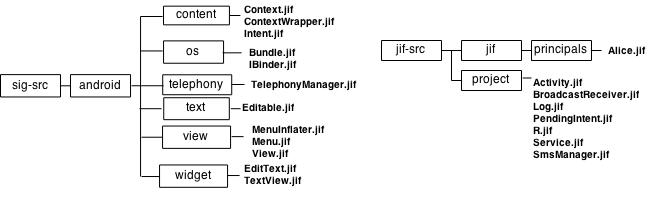
\includegraphics[width=12cm]{JifFilesystem.jpg}
	\end{center}
	\caption{Estructura de directorios en Jif.
	El código con anotaciones que se requiere para la evaluación de flujo de
	información en Jif, es alojado en los directorios sig-src y jif-src.}
	\label{fig:jifFilesystem} 
\end{figure}

\section{Ambiente y herramientas}
\textit{Versión de la API de Android}\newline
Las anotaciones a las clases de la API Android y las aplicaciones a anotar
mediante el prototipo, corresponden a la versión Android 4.2.2(API Level 17).

\textit{Versión del compilador de Jif}\newline
El componente que verifica el cumplimiento de las políticas de seguridad,
corresponde a la versión 3.4.2 del compilador de Jif.

\textit{Estructura de trabajo en JIF}\newline
El compilador de Jif maneja una estructura de directorios en la que se incluye
el código fuente .jif de las aplicaciones a analizar. Como ilustra la figura
\ref{fig:jifFilesystem} se tienen los directorios principales sig-src y jif-src.
El directorio sig-src está destinado para incluir librerías adicionales.\newline 
El directorio jif-src contiene todo el código jif correspondiente al programa
como tal que se va evaluar mediante Jif. Para los propósitos del presente
trabajo, se tienen los subdirectorios principals y project. En el subdirectorio
principals se incluyen las autoridades requeridas, y en el subdirectorio
project se incluyen, tanto las clases específicas de los aplicativos Android a
analizar, como las clases de que estos heredan como: Activity.jif, Service.jif,
etc.

\section{Compilación, integración y finalmente ejecución }
Las instrucciones para ejecutar la herramienta de análisis que se propone son
descritas en la sección \ref{sec:ejecutarPrototipo} de los anexos, allí se
ilustra paso a paso cómo ejecutar el anotador, y cómo compilar los aplicativos
a analizar mediante Jif.
    
\label{ch:evaluacion}
\chapter{Evaluación}
% Ventajas y limitaciones de la solución.\newline 
% Si aplica, evaluación de desempeño.  \newline 
% Si aplica, evaluación de usabilidad.  
% Hay otras soluciones similares? \newline 
% Cuáles son las diferencias y las ventajas y desventajas con respecto a esas soluciones.

\section{Consideraciones de evaluación}
El flujo de información es analizado al interior de una sola aplicación, no se
consideran flujos de información vía interApp, es decir, varias aplicaciones que
se comunican entre sí.

Cabe anotar que los resultados de evaluación que se presentan a continuación son
los obtenidos en el siguiente ambiente de pruebas: una máquina virtual con
sistema operativo Linux; 2,7 GHz de procesador y 1GB de Memoria RAM. En esa
misma máquina, se tiene instalada la versión 3.4.2 del compilador de Jif;
el artefacto de prueba para FlowDroid y JoDroid, obtenidos desde,
\cite{FlowDroid-artifact} y \cite{joDroidManual}, respectivamente.



\section{Conjunto de evaluación}
\label{sec:evalSet}

\begin{table}[t]
\small\addtolength{\tabcolsep}{-3pt}
\begin{tabular}{|p{13cm}|p{1cm}|}
	\hline
	\multicolumn{2}{|>{\columncolor[gray]{0.8}}c|}{\textbf{AndroidSpecific\_DirectLeak1}}\\
	\hline
	\textbf{Descripción} & \textbf{Leaks}\\
	\hline
	La variable \textit{mrg} tiene un nivel de seguridad alto,
	almacena información retornada por el método source \textit{getDeviceId}. Se
	genera flujo de información directo entre información con nivel de seguridad alto e
	información con nivel de seguridad bajo, al enviar como parámetro del método
	\textit{sendTextMessage}, información de la variable \textit{mrg}. & 1 \\
	\hline
	\multicolumn{2}{|>{\columncolor[gray]{0.8}}c|}{\textbf{AndroidSpecific\_LogNoLeak}}\\
	\hline
	\textbf{Descripción} & \textbf{Leaks}\\
	\hline
	El caso de prueba no presenta información con niveles de seguridad alto. Se
	presentan flujos de información entre información con el mismo nivel de
	seguridad, en este caso bajo, lo cual es permitido. & 0 \\
	\hline
	\multicolumn{2}{|>{\columncolor[gray]{0.8}}c|}{\textbf{ArraysAndLists\_ArrayAccess1}}\\
	\hline
	\textbf{Descripción} & \textbf{Leaks}\\
	\hline
	Se tiene un array en que se almacena información tanto proveniente como no
	proveniente de sources, parte de la información que almacena es enviada como
	parámetro del método \textit{sendTextMessage}. \textit{Observación:}
	Para la técnica de análisis de FlowDroid(taint analysis), se marca únicamente el
	índice del array donde se almacena el dato considerado como source, así,
	cuando se envía como parámetro del método \textit{sendTextMessage},
	el dato de un índice no marcado, no se genera leak. Para nuestra técnica
	de análisis(flujo de información mediante JIF), para que un array almacene
	información con nivel de seguridad alto, primero debe ser catalogo(anotado)
	con nivel de seguridad alto, lo que implica que el array podrá almacenar
	información tanto de nivel de seguridad alto como bajo, pero toda la
	información quedará con nivel de seguridad alto. En consecuencia, al enviar
	cualquier índice del array como parámetro del método
	\textit{sendTextMessage} se presenta un flujo de información no
	permitido. & 0
	\\
	\hline
% 	\multicolumn{2}{|>{\columncolor[gray]{0.8}}c|}{\textbf{GeneralJava\_Exceptions2}}\\
% 	\hline
% 	\textbf{Descripción} & \textbf{Leaks}\\
% 	\hline
% 	La variable \textit{imei} es de nivel de seguridad alto, almacena información
% 	devuelta por el método \textit{getDeviceId}. El control de flujo del
% 	programa conduce de manera implícita a la captura de una excepción tipo
% 	RuntimeException, desde allí se utiliza información proveída por la variable
% 	\textit{imei}, como parámetro para invocar el método \textit{sendTextMessage}.
% 	Generando un flujo de información indebido. & 1
% 	\\
% 	\hline
	\multicolumn{2}{|>{\columncolor[gray]{0.8}}c|}{\textbf{ImplicitFlows\_ImplicitFlow2}}\\
	\hline
	\textbf{Descripción} & \textbf{Leaks}\\
	\hline
	 La variable \textit{userInputPassword} con nivel de seguridad alto, almacena
	 información de un campo EditText tipo textPassword(password suministrado por
	 el usuario). Se generan flujos de información indebidos: al tratar de asignar
	 información a la variable passwordCorrect con nivel de seguridad bajo, a
	 partir de la comparación de información con nivel de seguridad alto(variable
	 textPassword), después, al tratar de mostrar en el \textit{log} información
	 que depende de tal comparación. & 1\\
	\hline
\end{tabular}
\caption{Aplicaciones de prueba.\newline
Describe parte del conjunto de aplicaciones de prueba. 
% Se considera con nivel de seguridad alto, variables y métodos que almacenan y modifican(respectivamente), información catalogada como privada(Sources).\newline
% Se considera con nivel de seguridad bajo, canales para envío de mensajes,
% muestra de logs y canales creados durante el control de flujo del programa.\newline 
}
\label{tab:descripApps0}
\end{table}

Para la evaluación se parte de DroidBech versión 1.0\cite{DroidBenchBenchmarks},
% benchmark integrado por 39 casos de prueba para aplicaciones Android, 
benchmark integrado por casos de prueba para aplicaciones Android, cuyos
autores son los mismos creadores de FlowDroid. Se opta por
utilizar DroidBench puesto que, en la literatura científica consultada al respecto, no se encuentran
otros benchmarks diseñados específicamente para evaluar aplicaciones Android.\newline 
De DroidBech se toma un grupo de testcases evaluables frente a la política de
seguridad establecida \ref{subsection:politica}, este grupo está integrado por
20 testcases. De los cuales, 14 presentan fugas de información.

La tabla \ref{tab:descripApps0} describe parte del grupo de testcases a
evaluar. En los casos en que se requiere, se precisan observaciones entre los
resultados de evaluación esperados para la técnica de análisis utilizada por
FlowDroid(análisis de flujo de datos) y la técnica de análisis propuesta en el
presente trabajo(análisis de flujo de información).
En la sección \ref{sec:testcases} de los anexos, se encuentra la
descripción del grupo de prueba completo.

El conjunto de prueba es analizado con FlowDroid, JoDroid y con el
Prototipo.\newline 
Los fundamentos\cite{Precision-Recall} para calificar los resultados del
análisis son los siguientes:\newline 
True Positive(TP) y False Positive(FP), para referenciar el número de Casos
Positivos esperados que son correcta o incorrectatamente identificados.\newline 
True Negatives(TN) y False Negatives(FN), para referenciar el número de 
Casos Negativos esperados que son correcta o incorrectamente
identificados.\newline
Ahora, para el contexto del presente análisis, donde se evalúa la detección de
fugas de información, los resultados del análisis reportados por cada
herramienta son calificados como:\newline 
True Positive(TP): cuando se reporta un leak que efectivamente existe.\newline
False Positive(FP): cuando se reporta un leak que no existe.\newline 
True Negative(TN): cuando no se reporta leak y efectivamente no existe.\newline
False Negative(FN): cuando no se reporta un leak existente. 

Una vez se tienen los resultados de análisis reportados por cada herramienta, se
calcula la Precisión y el Recall para cada una de ellas.

La \textbf{Precisión} hace referencia a los Casos Positivos esperados(correctos
e incorrectos: TP, FP), en contraste con la proporción de verdaderos Positivos(TP)
detectados\cite{Precision-Recall}. Una alta Precisión indica que la herramienta
reporta más correctos Positivos(TP) que incorrectos Positivos(FP). 

El \textbf{Recall} indica la proporción de Casos Positivos detectados(TP),
frente a los Casos Positivos esperados como correctos\cite{Precision-Recall}. Un
alto Recall indica que la herramienta reporta más correctos Positivos(TP) que incorrectos
Negativos(FN). Es decir, la herramienta deja pasar menos errores.\newline
% La Precisión(\ref{pre}) mide la cantidad de respuestas válidas(TP), frente al
% total de respuestas, esto es, respuestas válidas(TP) y respuestas no válidas(FP).
% A mayor Precisión, la herramienta reporta más verdaderos positivos(TP) y menos
% falsos positivos(FP). En otras palabras, de los leaks existentes, la
% herramienta reporta una mayor cantidad.
% 
% Con el Recall(\ref{rec}) se mide la cantidad de respuestas válidas(TP), frente
% al total de respuestas válidas(TP) y respuestas válidas no detectadas(FN). A
% mayor Recall, menor reporte de falsos negativos.\newline

Las fórmulas para calcular Precisión(p) y Recall(r), son:
\begin{equation}
\label{pre}
	p = TP/(TP +FP) 
\end{equation}
\begin{equation}
\label{rec}
	r = TP/(TP+FN)
\end{equation}
Donde: \newline
TP representa el total de verdaderos positivos; FP corresponde al total de
falsos positivos y  FN representa el total de falsos
negativos; reportados por la herramienta.

% Las formulas \ref{p} y \ref{r}, permiten el calculo de ambas métricas
% de seguridad.\newline
Además de las fórmulas anteriormente descritas, se utiliza el comando
\textit{time}\cite{time-man} de unix, para medir el desempeño de cada
herramienta.

\section{Evaluación FlowDroid y Prototipo } 
\label{subsec:fvsp}
Del total de testcases(20), 14 presentan fugas de información mientras que 6 de
ellos no. Los resultados de evaluación para FlowDroid y el Prototipo, son
presentados en la tabla \ref{tb:resultados}. En esta, por cada caso de prueba
se indica la cantidad de leaks que presenta, el resultado devuelto por la
herramienta y el tiempo que tarda el análisis.

\begin{table}[H]
\begin{center}
\small\addtolength{\tabcolsep}{-3pt}
\begin{tabular}{|p{1cm}|p{6cm}|p{1cm}|p{1cm}|p{1cm}|p{1cm}|p{1cm}|}
	\hline
	\textbf{Item} & \textbf{Testcase} & \textbf{Leaks} & \textbf{F} &
	\textbf{P} & \textbf{ tF} & 
	\textbf{tP}\\
	\hline
	1 & AndroidSpecific\_DirectLeak1 & 1 & TP & TP &5.371s &2.063s\\
	\hline
	2 & AndroidSpecific\_InactiveActivity & 0 & TN & FP  &3.255s &2.469s\\
	\hline
	3 & AndroidSpecific\_LogNoLeak & 0 & TN & TN &5.505s &2.946s\\
	\hline
	4 & AndroidSpecific\_Obfuscation1 & 1 & TP & TP &6.734s &2.706s\\
	\hline
	5 & AndroidSpecific\_PrivateDataLeak2 & 1 & TP & TP & 6.144s &2.644s\\
	\hline
	6 & ArraysAndLists\_ArrayAccess1 & 0 & FP & FP & 4.708s & 1.278s\\
	\hline
	7 & ArraysAndLists\_ArrayAccess2 & 0 & FP & FP & 4.4s &1.361s\\
	 \hline
	8 & GeneralJava\_Exceptions1 & 1 & TP & TP &6.397s &2.755s\\
	\hline
	9 &  GeneralJava\_Exceptions2 & 1 & TP & TP &5.887s &1.980s\\
	\hline
	10 & GeneralJava\_Exceptions3 & 0 & FP & FP &6.008s &2.032s\\
	\hline
	11 & GeneralJava\_Exceptions4 & 1 & TP & TP &5.731s &2.313s\\
	\hline
	12 & GeneralJava\_Loop1 & 1 & TP & TP &5.605s &2.800s\\
	\hline
	13 & GeneralJava\_Loop2 & 1 & TP & TP &4.719s &1.361s\\
	\hline
	14 & GeneralJava\_UnreachableCode & 0 & TN & FP &3.792s &1.197s\\
	\hline
	15 & ImplicitFlows\_ImplicitFlow1 & 1 & FN & TP &4.853s &1.331s\\
	\hline
	16 & ImplicitFlows\_ImplicitFlow2 & 1 & FN & TP &4.496s &1.212s\\
	\hline
	17 & ImplicitFlows\_ImplicitFlow4 & 1 & FN & TP &4.375s &1.224s\\
	\hline
	18 & Lifecycle\_ActivityLifecycle3 & 1 & TP & TP &4.792s &1.222s\\
	\hline
	19 & Lifecycle\_BroadcastReceiverLifecycle1 & 1 & TP & TP &4.456s &1.061s\\
	\hline
	20 & Lifecycle\_ServiceLifecycle1 & 1 & TP & TP &5.225s &1.180s\\
	\hline
\end{tabular}
\end{center}
\caption{Resultados de evaluación para FlowDroid y Prototipo. Donde
\textit{Item} indica el testcase que se evalúa, \textit{Testcase} especifica el
nombre de la aplicación para el caso de prueba; \textit{Leaks} indica si el
testcase presenta fugas de información; \textit{F} y  \textit{P} muestran los
resultados devueltos por FlowDroid y por el Prototipo; \textit{tF} y
\textit{tP}, señalan el tiempo(en segundos) que toma el análisis para Flowdroid
y para el Prototipo, respectivamente.}
\label{tb:resultados}
\end{table}

\subsection{Análisis de evaluación entre FlowDroid y Prototipo}
\subsubsection{Resultados de desempeño}
% -\textit{Resultados de desempeño}\newline
Acorde a los tiempos señalados en los campos tF y tP de la tabla
\ref{tb:resultados}, en promedio, FlowDroid tarda 3,3 segundos más que el
Prototipo para ejecutar el análisis.

% PULIR IDEAAAAA***\newline
% Tal diferencia de tiempo va en concordancia con los costos de ejecución que
% implica una u otra técnica de análisis, mientras el análisis de flujo de
% información basado en lenguajes tipados de seguridad(que es lo que se evalua
% mediante el prototipo) sólo requiere llegar hasta el chequeo de tipos, la
% técnica de analisis de flujo de datos en que se basa FlowDroid utiliza
% algoritmos de orden O(ED)3 , cuya complejidad es de orden polinomial,
% O(ED)3\cite[page 3]{FCO-PDG}.\newline
% Se podría destacar como positivo que el análisis de flujo de información
% mediante técnicas de tipado de seguridad, requiere menos tiempo que la técnica
% de marcado de datos utilizada por FlowDroid.x
\subsubsection{Falsos positivos, precisiones}
% -\textit{Resultados de precisión}\newline
En lo que respecta a los resultados del Prototipo, los FP correspondientes a los
items 2 y 14 de la tabla \ref{tb:resultados}, surgen como consecuencia de un
diseño de análisis pesimista (evaluación del flujo de información
\ref{subsec:consVerPol}), donde se asume que todos los métodos definidos en
la clase serán invocados. Por consiguiente, todos los métodos son incluidos para
el análisis del flujo de información. Así, si los métodos conllevan a flujos de
datos indebidos, independientemente de si son invocados o no, son considerados
como generadores de fugas de información.\newline 
% En lo que respecta a los resultados del Prototipo, los FP correspondientes a los
% items 2(AndroidSpecific\_InactiveActivity) y 14(GeneralJava\_UnreachableCode) de
% la tabla \ref{tb:resultados}, los cuales presentan flujos de información
% indebidos, pero en realidad nunca tendran lugar, porque se presentan en: una
% actividad que no está activada en el Manifest, y un método que nunca es llamado.
% Dan lugar al reporte de falsos positivos por parte del Prototipo, puesto que
% al basarse en un análisis pesimista (evaluación del flujo de información
% \ref{subsec:consVerPol}), donde se asume que todos los métodos definidos en la
% clase serán invocados. Por consiguiente, todos los métodos son incluidos para el
% análisis del flujo de información. Así, si los métodos conllevan a flujos
% de datos indebidos, independientemente de si son invocados o no, son
% considerados como generadores de fugas de información.\newline 
Por otro lado, en el caso de ArraysAndLists: items 6 y 7, de la tabla
\ref{tb:resultados}, no es sencillo calificar los resultados como FP, puesto
que, para lo que está analizando FlowDroid(verificar que su técnica de análisis
diferencie entre los elementos marcados y no marcados de un array),
efectivamente se presentan FP, sin embargo, para la forma en que se deben
implementar los programas en Jif, donde se suele definir un nivel de seguridad
para todo el array antes de almacenar los elementos en el mismo, podría decirse
que no se trata de un FP, porque se revelo información que había sido catalogada
con nivel de seguridad alto.

\subsubsection{Detección de flujos implícitos}
A diferencia de FlowDroid, el Prototipo detecta fugas de información través de
flujos implícitos. La no detección de Flujos implícitos por parte de FlowDroid,
responde al tipo de análisis y las técnicas en que se fundamenta la herramienta:
análisis de flujo de datos mediante técnicas tainting. Basada en 
%Puesto que, 
% 
% \newline
% --el Prototipo, la anotación generada por el prototipo, o la técnica de análisis
% en que se basa el diseño de la solución: lenguajes tipados de seguridad???
% 
% -\textit{Acerca de por qué FlowDroid no detecta flujos implícitos}\newline
%el análisis de FlowDroid utiliza  técnicas DataFlow, específicamente, utiliza
% tainting análisis.
% Para hacer seguimiento al flujo de información de un
% programa, la técnica de análisis tainting se basa en: 
asociar una o más marcas
con el valor de los datos en el programa, y en propagarlas. Dependiendo de los
criterios definidos para el análisis, la marca puede ser propagada a causa de
flujos explícitos o de flujos implícitos\cite{taint-analysis}, o a causa de
ambos. En flujos explícitos la propagación ocurre cuando el valor de una variable marcada está
implicada en el calculo de otra variable. En flujos implícitos la propagación
tiene lugar a través de dependencias en el control de flujo del programa, por
ejemplo, cuando el valor de un dato marcado afecta indirectamente otra variable.\newline 
En el caso de FlowDroid, los criterios que fundamentan el análisis de la
herramienta, hacen que el marcado de datos se propague para flujos explícitos y
y no para flujos implícitos. Por consiguiente, FlowDroid no detecta flujos
implícitos.\newline
Con esto presente, se definen dos escenarios de análisis: Precisión y Recall,
incluyendo flujos implícitos; y  Precisión y Recall, excluyendo flujos
implícitos, donde se incluyen u omiten los testcases para flujos
implícitos(items 15 a 17, tabla \ref{tb:resultados}).\newline
La tabla \ref{tb:FlowDroidPrototipoFI} muestra los resultados de evaluación para
ambos casos.\newline
%En el caso de TaintDroid, tampoco detecta flujos implícitos, porque entre las
% desiciones de diseño de la herramienta está enfocarse en el seguimeinto al
% flujo de datos y no al flujo de control, puesto que si incluyen seguimiento al
% flujo de control, se adiciona sobrecarga a la herramienta, la cual es de tipo
% dinámico.
\begin{table}[H]
\begin{center}
\begin{tabular}{c|c|c|c|c|}
\cline{2-5}
& \multicolumn{2}{>{\columncolor{gray!30}} c  }{\multirow{1}{*}{Con FI}}
& \multicolumn{2}{|c|}{\multirow{1}{*}{\cellcolor{gray!50} {Sin FI}}}\\
\cline{2-5}
& \cellcolor{gray!30}FlowDroid & \cellcolor{gray!30}Prototipo &
\cellcolor{gray!50}FlowDroid & \cellcolor{gray!50}Prototipo \\
\cline{1-5}
\multicolumn{0}{ |c|  }{\multirow{0}{*}{FP} }  & 3 & 5 & 3 & 5\\ \cline{0-4}
\multicolumn{0}{ |c|  }{\multirow{0}{*}{FN} }  & 3 & 0 & 0 & 0\\ \cline{0-4}
\multicolumn{0}{ |c|  }{\multirow{0}{*}{TP} }  & 11 & 14 & 11 & 11 \\
\cline{0-4}
\multicolumn{0}{ |c|  }{\multirow{0}{*}{TN} }  & 3 & 1 &  3 & 1\\ \cline{0-4}
\end{tabular}
\end{center}
\caption{Resultados de precisión para FlowDroid y Prototipo, de acuerdo al
escenario, incluyendo o excluyendo flujos implícitos(FI). Resume el total de
falsos positivos(FP), verdaderos positivos(TP), verdaderos negativos(TN) y falsos
negativos(FN); obtenidos tanto con FlowDroid como con el Prototipo.}
\label{tb:FlowDroidPrototipoFI}
\end{table}


\subsubsection{Precisión y Recall, incluyendo flujos implícitos}
% \textit{Precisión y Recall, incluyendo flujos implícitos}\newline
Los resultados obtenidos en la tabla \ref{tb:FlowDroidPrototipoFI} señalan que
de las 14 fugas existentes, el Prototipo las detecta todas, presenta 14
TP(verdaderos positivos); mientras que, FlowDroid deja pasar 3.\newline
Por otro lado, el Prototipo presenta más falsos positivos que FlowDroid, de los
6 testcases que no presentan leaks, el prototipo reporta 5 como si fuesen
fugas, mientras que FlowDroid reporta 3.\newline
Así, en lo que respecta a Precisión, FlowDroid presenta un porcentaje del
78,57\%, siendo más preciso frente al Prototipo, que presenta un porcentaje del
73,68\%.\newline 
Por otro lado, el Prototipo presenta un porcentaje en Recall del 100\%,
mientras que FlowDroid presenta un porcentaje del 78,75\%.

\subsubsection{Precisión y Recall, excluyendo flujos implícitos}
% \textit{Precisión y Recall, excluyendo flujos implícitos}\newline
Excluyendo los testcases para flujos implícitos, el conjunto de prueba se reduce
a 17 casos. De los cuales, 11 presentan leaks.\newline 
En este contexto, el porcentaje de Precisión para FlowDroid es de 78,57\%,
mientras que para el Prototipo es del 68,75\%. El porcentaje de Recall es igual
para FlowDroid y el Prototipo: 100\%.


\section{Evaluación JoDroid y Prototipo}
% Del conjunto de casos de prueba JoDroid ignora las excepciones, ya que su actual
% implementación no soporta análisis del flujo de información a través de
% tales sentencias[pag 93 \cite{JoDroid-Thesis}]. Por tanto, los testcases
% GeneralJava\_Exceptions1 a GeneralJava\_Exceptions4, no son evaluados. 
% No obstante, para calcular la precisión y el recall se consideran dos
% escenarios, uno en que se incluyen y otra en que no.
La tabla \ref{tab:JoDroid-Prototipo} ilustra los resultados de evaluación para JoDroid y el
Prototipo, en base a los cuales, se calculan las métricas de precisión y recall. 
\label{subsec:jvsp}
\begin{table}[t]
\begin{center}
\small\addtolength{\tabcolsep}{-3pt}
\begin{tabular}{|p{0.8cm}|p{6cm}|p{1cm}|p{0.8cm}|p{0.8cm}|p{1,8cm}|p{1cm}|}
	\hline
	\textbf{Item} & \textbf{Testcase} & \textbf{Leaks} & \textbf{J} &
	\textbf{P} & \textbf{ tJ} & \textbf{tP}\\
	\hline
	1 & AndroidSpecific\_DirectLeak1 & 1 & TP & TP & 22m11.991s &2.063s\\
	\hline
	2 & AndroidSpecific\_InactiveActivity & 0 & FP & FP  & 22m25.617s &2.469s\\
	\hline
	3 & AndroidSpecific\_LogNoLeak & 0 & TN & TN & 21m6.548s &2.946s\\
	\hline
	4 & AndroidSpecific\_Obfuscation1 & 1 & TP & TP &22m46.541s&2.706s\\
	\hline
	5 & AndroidSpecific\_PrivateDataLeak2 & 1 & TP & TP &21m32.447s&2.644s\\
	\hline
	6 & ArraysAndLists\_ArrayAccess1 & 0 & FP & FP &22m01.926s& 1.278s\\
	\hline
	7 & ArraysAndLists\_ArrayAccess2 & 0 & FP & FP &22m11.023s&1.361s\\
	 \hline
	8 & GeneralJava\_Exceptions1 & 1 & FN & TP & 22m52.134s &2.755s\\
	\hline
	9 & GeneralJava\_Exceptions2 & 1 & FN & TP & 21m4.434s&1.980s\\
	\hline
	10 & GeneralJava\_Exceptions3 & 0 & TN\tablefootnote{Al igual que en
	el resto de testcases para GeneralJava\_Exceptions(items 8, 9 y 11), la
	herramienta no detecta leaks, la diferencia para el presente caso, es que efectivamente no existe leak. Por tanto se califica como TN.} & FP & 21m37.040s &2.032s\\
	\hline
% 	\hline
% 	GeneralJava\_Exceptions3 & 0 & TN & FP & 21m37.040s &2.032s\\
% 	\hline
	11 & GeneralJava\_Exceptions4 & 1 & FN  & TP & 21m10.240s &2.313s\\
	\hline
	12 & GeneralJava\_Loop1 & 1 & TP & TP &21m15.30s&2.800s\\
	\hline
	13 & GeneralJava\_Loop2 & 1 & TP & TP &21m41.224s&1.361s\\
	\hline
	14 & GeneralJava\_UnreachableCode & 0 & TN & FP &22m84.138s&1.197s\\
	\hline
	15 & ImplicitFlows\_ImplicitFlow1 & 1 & TP & TP &22m55.645s&1.331s\\
	\hline
	16 & ImplicitFlows\_ImplicitFlow2 & 1 & TP & TP &22m32.231s&1.212s\\
	\hline
	17 & ImplicitFlows\_ImplicitFlow4 & 1 & TP & TP &22m43.110s&1.224s\\
	\hline
	18 & Lifecycle\_ActivityLifecycle3 & 1 & TP & TP &22m54.651s&1.222s\\
	\hline
	19 & Lifecycle\_BroadcastReceiverLifecycle1 & 1 & TP & TP &22m42.347s&1.061s\\
	\hline
	20 & Lifecycle\_ServiceLifecycle1 & 1 & TP & TP &22m92.722s&1.180s\\
	\hline
\end{tabular}
\end{center}
\caption{Resultados de evaluación para JoDroid y Prototipo. Donde
\textit{Testcase} especifica el nombre de la aplicación que se está evaluando;
\textit{Leaks} indica si el testcase presenta fugas de información; \textit{J} y
\textit{P} muestran los resultados devueltos por JoDroid y por el Prototipo;
\textit{tJ} y \textit{tP}, señalan el tiempo que toma el análisis para JoDroid
y para el Prototipo, respectivamente.}
\label{tab:JoDroid-Prototipo}
\end{table}

\subsection{Análisis de evaluación entre JoDroid y Prototipo}
\subsubsection{Resultados de desempeño}
% -\textit{Resultados de desempeño}\newline
Para el análisis mediante JoDroid se deben seguir una serie de pasos, tal como
se describen en el manual de referencia\cite{joDroidManual}, de estos,
únicamente se toma el tiempo correspondiente al paso para generar el
grafo de dependencia del programa(PDG), del cual parte el análisis. En general,
el tiempo que tarda la generación del PDG para cada aplicación analizada, oscila
entre 21 y 22 minutos. Cabe anotar que estos valores podrían cambiar con otras
características de hardware, sin embargo, asignando 1 GB de Ram a la máquina
virtual de Java, para la generación del PDG, es ese el rango de tiempo obtenido.
En consecuencia, para los valores de tiempo que señala la presente evaluación,
es posible decir que la herramienta es costosa en desempeño.

\subsubsection{Detección de Flujos implícitos}
% -\textit{Resultados de Precisión}\newline
La tabla \ref{tab:JoDroid-Prototipo} muestra que al igual que el Prototipo,
JoDroid detecta fugas de información a través de flujos implícitos. Ya que,
en los testcases correspondientes a flujos implícitos, items 15, 16 y 17, ambas
herramientas detectan que efectivamente, se presentan fugas de
información.\newline

\subsubsection{Fugas a través de excepciones}
Es importante resaltar que del conjunto de casos de prueba, JoDroid ignora el
control de flujo de información para excepciones(items 8 a 11 de la tabla
\ref{tab:JoDroid-Prototipo}), puesto que, su actual implementación no soporta
análisis del flujo de información a través de tales sentencias[pag 93
\cite{JoDroid-Thesis}].
En la tabla \ref{tb:jodroidP2exce} se muestran dos escenarios para los
resultados de evaluación: Con  excepciones y Sin excepciones. 
Con base en tales resultados se calcula la Precisión y Recall para cada uno de
los escenarios.

\begin{table}[t]
\begin{center}
\begin{tabular}{c|c|c|c|c|}
\cline{2-5}
& \multicolumn{2}{>{\columncolor{gray!30}} c  }{\multirow{1}{*}{Con
excepciones}} & \multicolumn{2}{|c|}{\multirow{1}{*}{\cellcolor{gray!50} {Sin
excepciones}}}\\
\cline{2-5}
& \cellcolor{gray!30}JoDroid & \cellcolor{gray!30}Prototipo &
\cellcolor{gray!50}JoDroid & \cellcolor{gray!50}Prototipo \\
\cline{1-5}
\multicolumn{0}{ |c|  }{\multirow{0}{*}{FP} }  & 3 & 5 & 3 & 4\\ \cline{0-4}
\multicolumn{0}{ |c|  }{\multirow{0}{*}{FN} }  & 3 & 0 & 0 & 0\\ \cline{0-4}
\multicolumn{0}{ |c|  }{\multirow{0}{*}{TP} }  & 11 & 14 & 11 & 11 \\
\cline{0-4}
\multicolumn{0}{ |c|  }{\multirow{0}{*}{TN} }  & 3 & 1 &  2 & 1\\ \cline{0-4}
\end{tabular}
\end{center}
\caption{Resultados de precisión para JoDroid y Prototipo. Muestra los
escenarios en que mide. Resume el total de falsos positivos(FP), verdaderos
positivos(TP), verdaderos negativos(TN) y falsos negativos(FN); obtenidos tanto
con JoDroid como con el Prototipo.}
\label{tb:jodroidP2exce}
\end{table}

\subsubsection{Precisión y Recall incluyendo excepciones}
% \textit{Precisión y Recall incluyendo excepciones}\newline
Del total de testcases(20), 14 presentan fugas de información. 
De los casos con fuga de información, 3 corresponden a las excepciones
incluidas(items 8 a 11, tabla \ref{tab:JoDroid-Prototipo}), y se califican como
falsos negativos(FN) porque JoDroid no los detecta. La tabla
\ref{tb:jodroidP2exce} ilustra los resultados de evaluación.\newline 
En cuanto a la Precisión(p), JoDroid presenta un porcentaje del 78,57\%,
mientras que el Prototipo presenta un porcentaje del  73,68\%.\newline
En cuanto a Recall(r), el Prototipo presenta un porcentaje del 100\%, frente a
un porcentaje del 78,57\% presentado por JoDroid.

\subsubsection{Precisión y Recall excluyendo excepciones}
% \textit{Precisión y Recall excluyendo exceptions}\newline
Omitiendo los testcases para excepciones(items 8 a 11, tabla
\ref{tab:JoDroid-Prototipo}), el total de testcases(20) queda reducido a 16. 
De estos, 11 presentan fugas de información.\newline 
En lo que respecta a la métrica de Precisión, JoDroid presenta un porcentaje del
78,57\%; frente al Prototipo que presenta un porcentaje del 73,33\%.\newline 
Para la métrica de Recall, tanto JoiDroid como el Prototipo, presentan el mismo
porcentaje esto es 100\%.\newline



\section{Análisis de evaluación FlowDroid, JoDroid, Prototipo}
\label{subsec:fjp}
%las tablas confirman lo que ya se sabia segun la literatura existe.

\begin{table}[h]
\begin{center}
\begin{tabular}{c|c|c|c|}
\cline{2-4}
& \cellcolor{gray!30}FlowDroid & \cellcolor{gray!30}JoDroid &
\cellcolor{gray!30}Prototipo \\
\cline{1-4}
\multicolumn{0}{ |c|  }{\multirow{0}{*}{FP} }  & 3 & 3 & 5\\ \cline{0-3}
\multicolumn{0}{ |c|  }{\multirow{0}{*}{FN} }  & 3 & 3 & 0\\ \cline{0-3}
\multicolumn{0}{ |c|  }{\multirow{0}{*}{TP} }  & 11 & 11 & 14\\\cline{0-3}
\multicolumn{0}{ |c|  }{\multirow{0}{*}{TN} }  & 3 & 3 &  1\\ \cline{0-3}
\end{tabular}
\end{center}
\caption{Resultados de precisión para FlowDroid y Prototipo. Resume el total de
falsos positivos(FP), verdaderos positivos(TP), verdaderos negativos(TN) y
falsos negativos(FN).}
\label{tb:porcentajes}
\end{table}

\begin{table}[h]
\begin{center}
\begin{tabular}{cc|c|c|c}
\cline{2-4}
& \multicolumn{0}{ |c|  }{\multirow{1}{*}{\cellcolor{gray!30} FlowDroid} } &
\cellcolor{gray!30}JoDroid & \cellcolor{gray!30}Prototipo \\
\cline{1-4}
\multicolumn{0}{ |c|  }{\multirow{0}{*}{Precisión} }  & 78,57\% & 78,57\% & 73,68\%
\\
\cline{0-3}
\multicolumn{0}{ |c|  }{\multirow{0}{*}{Recall} }  & 78,57 & 78,57\% &  100\%\\
\cline{0-3}
\multicolumn{0}{ |c|  }{\multirow{0}{*}{Detección Flujos Implícitos} }  & No &
Si & Si\\
\cline{0-3}
\end{tabular}
\end{center}
\caption{Comparación entre FlowDroid, JoDroid y Prototipo. Ilustra los
porcentajes para Precisión, Recall, y la detección de leaks mediante
flujos implícitos.\newline}
\label{tb:comparacion}
\end{table}


En base a los resultados para el conjunto de
evaluación(compuesto por 20 testcases, de los cuales 14 presentan leaks),
obtenidos en los anteriores apartados, 
% donde se presentó un análisis detallado para la evaluación entre FlowDroid vs
% Prototipo, y, JoDroid vs Prototipo; 
se comparan las tres herramientas: FlowDroid, JoDroid y Prototipo, frente a 
Precisión, Recall, y la detección de fugas de información mediante flujos
implícitos. La tabla \ref{tb:porcentajes} ilustra todos los resultados y la
tabla \ref{tb:comparacion} ilustra los respectivos porcentajes.\newline

% \begin{table}[b]
% \begin{center}
% \begin{tabular}{c|c|c|c|}
% \cline{2-4}
% & \cellcolor{gray!30}FlowDroid & \cellcolor{gray!30}JoDroid &
% \cellcolor{gray!30}Prototipo \\
% \cline{1-4}
% \multicolumn{0}{ |c|  }{\multirow{0}{*}{FP} }  & 3 & 3 & 5\\ \cline{0-3}
% \multicolumn{0}{ |c|  }{\multirow{0}{*}{FN} }  & 3 & 3 & 0\\ \cline{0-3}
% \multicolumn{0}{ |c|  }{\multirow{0}{*}{TP} }  & 11 & 11 & 14\\\cline{0-3}
% \multicolumn{0}{ |c|  }{\multirow{0}{*}{TN} }  & 3 & 3 &  1\\ \cline{0-3}
% \end{tabular}
% \end{center}
% \caption{Resultados de precisión para FlowDroid y Prototipo. Resume el total de
% falsos positivos(FP), verdaderos positivos(TP), verdaderos negativos(TN) y
% falsos negativos(FN).}
% \label{tb:porcentajes}
% \end{table}
% 
% \begin{table}[b]
% \begin{center}
% \begin{tabular}{cc|c|c|c}
% \cline{2-4}
% & \multicolumn{0}{ |c|  }{\multirow{1}{*}{\cellcolor{gray!30} FlowDroid} } &
% \cellcolor{gray!30}JoDroid & \cellcolor{gray!30}Prototipo \\
% \cline{1-4}
% \multicolumn{0}{ |c|  }{\multirow{0}{*}{Precisión} }  & 78\% & 78,57\% & 73,68\%
% \\
% \cline{0-3}
% \multicolumn{0}{ |c|  }{\multirow{0}{*}{Recall} }  & 78\% & 78,57\% &  100\%\\
% \cline{0-3}
% \multicolumn{0}{ |c|  }{\multirow{0}{*}{Detección Flujos Implícitos} }  & No &
% Si & Si\\
% \cline{0-3}
% \end{tabular}
% \end{center}
% \caption{Comparación entre FlowDroid, JoDroid y Prototipo. Ilustra los
% porcentajes para Precisión, Recall, y la detección de leaks mediante
% flujos implícitos.\newline}
% \label{tb:comparacion}
% \end{table}

\textbf{\textit{Desempeño}}\newline 
Como muestran las tablas \ref{tb:resultados} y \ref{tab:JoDroid-Prototipo}, el
Prototipo presenta mejor desempeño frente FlowDroid y JoDroid. En el caso de
FlowDroid, en promedio tarda 3,3 segundos más que el Prototipo para ejecutar el
análisis. En el caso de JoDroid, el tiempo de análisis es costoso en comparación
a las otras herramientas, puesto que su tiempo de ejecución oscila entre 21 y 22
minutos.\newline

% EXPLICAR POR QUE, DE ACUERDO A LA TECNICA DE ANALISIS?\newline
% Como muestran las tablas \ref{tb:resultados} y \ref{tab:JoDroid-Prototipo}, el
% análisis de flujo de información basado en lenguajes tipados de seguridad(en que
% se fundamenta la propuesta de análisis) presenta un mejor desempeño, frente a
% las técnicas en que se basan FlowDroid y JoDroid, análisis de flujo de datos
% mediante técnicas tainting y IFC(Information Flow Control) mediante PDG y
% slicing, respectivamente.
\textbf{\textit{Precisión y Recall}}\newline
Tanto FlowDroid como JoDroid presentan mejor Precisión que el Prototipo, es
decir que el Prototipo presenta más falsos positivos(FP).\newline 
Por otro lado, el Prototipo presenta mayor Recall frente a FlowDroid y JoDroid,
por tanto, el Prototipo detecta mayor cantidad de fugas existentes (reporta
menos FN).
Para este caso particular, el Prototipo detecta todos los TP.\newline 
En consecuencia, es posible decir que aunque el Prototipo presenta mayor
cantidad de FP frente a FlowDroid y JoDroid, deja pasar menos fugas de
información.\newline
En lo que respecta a flujos implícitos, a diferencia de FlowDroid, tanto JoDroid
como el Prototipo detectan fugas de información a través de Flujos
implícitos.\newline

% EXPLICAR POR QUE DE ACUERDO A LAS TECNICAS DE ANALISIS?\newline
% El análisis de flujo de información mediante lenguajes tipados de
% seguridad(en que se basa el Prototipo), ofrece un mejor Recall que
% FlowDroid, sin embargo FlowDroid es más preciso. Esto se traduce en que la
% propuesta de análisis evaluada a través del Prototipo, presenta más falsos
% positivos que FlowDroid, pero no deja pasar fugas de información.\newline
% Por otro lado, el Prototipo detecta fugas de información presentes en Flujos
% implicitos, FlowDroid No.\newline
% El análisis de flujo de información mediante lenguajes tipados de seguridad,
% ofrece igual Recall que la técnica de PDG utilizada por JoDroid, sin
% embargo, JoDroid presenta mejor Precisión.\newline
\textbf{\textit{Análisis métricas acorde al tipo de análisis}}\newline
Analizando los resultados para las métricas de desempeño, precisión y recall;
descritas anteriormente, acorde al tipo de análisis y técnicas en que se basa
cada herramienta, es posible anotar:\newline 

- Desempeño:\newline 
El prototipo presenta mejor desempeño, como resultado de analizar flujo de
información mediante lenguajes tipados de seguridad, más específicamente a
través de Jif. Dado que Jif recurre a técnicas de compilación(label checking) y
no requiere la generación de grafos de dependencia, el análisis toma menos
tiempo.

-Precisión, Recall y detección de Flujos implícitos:\newline 
el análisis pesimista en que se basa el Prototipo, donde se asume que todos los
métodos implementados en la aplicación serán invocados, hace que los resultados
del análisis sean menos precisos, generando más falsos positivos(FP). 
%En consecuencia, se tiene un análisis unsound?.\newline 
%%VERIFICAR SENSIBILIDAD AL CONTEXTO,,,,
%(EL ANÁLISIS PESIMISTA O LA TECNICA DE LENGUAJES TIPADOS?)
Para la evaluación realizada, el análisis de flujo de información mediante el
sistema de anotaciones de Jif, ofrece un mejor recall, frente a: el análisis de
flujo de datos en que se basa FlowDroid y el análisis de flujo de información
mediante System Dependences Graphs  en que se basa JoDroid. Esto hace que para
el experimento, la técnica de análisis del prototipo sea completa(completeness),
puesto que, dentro de los leaks detectados están todos los leaks que
efectivamente existen.\newline
Una ventaja de las técnicas basadas en control de flujo de información es que al
analizar tanto flujos explícitos como flujos implícitos, detectan la generación
de leaks mediante flujos implícitos casi de forma natural, contrario a lo que
sucede en las técnicas de análisis de flujos de datos, en la cuales, sino se
propaga el marcado de datos a través de flujos implícitos, no es posible
detectar fugas de datos a través de los mismos.

Los resultados de evaluación confirman las hipótesis iniciales del presente
trabajo, según las cuales se esperaba que: al hacer análisis de flujo de
información mediante lenguajes tipados de seguridad, los resultados del análisis
fuesen más rápidos pero menos precisos, reportando más falsos positivos que
JoDroid y FlowDroid.\newline
Tal resultado refleja lo ilustrado por la teoría \cite{taghdiri-etal-2010} y
\cite{hammer09ijis}.\newline

La tabla \ref{tab:resumen} resume 
las ventajas, desventajas, similitudes y
diferencias entre el Prototipo y las herramientas de comparación, FlowDroid y
JoDroid, respectivamente. En esta se ilustra por ejemplo, como el prototipo
detecta automáticamente los sources y sinks, mientras que JoDroid no.

\begin{table}[H]
%\begin{center}
\small\addtolength{\tabcolsep}{-3pt}
%\begin{tabular}{|p{4cm}|p{1cm}|p{1cm}|}
\begin{tabular}{|p{4cm}|p{1cm}|p{1cm}|p{1cm}|p{1cm}|p{1cm}|p{1cm}|p{1cm}|p{1cm}|}
	\hline
	{\multirow{2}{*}{\textbf{Item}}}
	&\multicolumn{4}{c|}{\cellcolor{gray!30}\textbf{Prototipo vs FlowDroid}} &
	\multicolumn{4}{c|}{\cellcolor{gray!55}\textbf{Prototipo vs JoDroid}}\\
	\cline{2-9}
	 & \cellcolor{gray!30}\tiny{\textbf{ventaja}} &
	 \cellcolor{gray!30}\tiny{\textbf{desvent}} &
	 \cellcolor{gray!30}\tiny{\textbf{similit}}&
	 \cellcolor{gray!30}\tiny{\textbf{diff}} &
	 \cellcolor{gray!55}\tiny{\textbf{ventaja}} &
	 \cellcolor{gray!55}\tiny{\textbf{desvent}} &
	 \cellcolor{gray!55}\tiny{\textbf{similit}}&
	 \cellcolor{gray!55}\tiny{\textbf{diff}}\\
	\hline
	\footnotesize{Menor Precisión} & &\checkmark & & & &\checkmark& &\\
	\hline
	Mayor Recall &\checkmark& & & &\checkmark& & &\\
	\hline
	Menor costo en desempeño & & & & &\checkmark& & &\\
	\hline
	Bajo costo en desempeño & & &\checkmark& & & & & \\
	\hline
	Detección de flujos implícitos & \checkmark& & & & & &\checkmark&\\
	\hline
	No detección automática de sources y sinks & &\checkmark&& &&&\checkmark& \\
	\hline
	No soporte para Análisis interApp & &\checkmark& & & & &\checkmark&\\
	\hline
	\footnotesize{Tipo de análisis(flujo de información; flujo de datos)} & & &
	&\checkmark& & & &\\
	\hline
	Tipo de análisis IFC & & & & & & &\checkmark&\\
	\hline
	Técnica de análisis: PDG, slicing & & & & & & & &\checkmark\\
	\hline
\end{tabular}
%\end{center}
\caption{Síntesis ventajas, desventajas, similitudes y diferencias; del
Prototipo frente a FlowDroid y JoDroid(respectivamente).\newline}
\label{tab:resumen}
\end{table}

\section{Tipos de análisis y técnicas evaluadas}
% En las subsecciones anteriores(4.2.1 a 4.2.3), se analizaron los resultados de
% evaluación con respecto a un conjunto de aplicaciones específico. En la presente
% sección, el análisis se basa en las herramientas previamente evaluadas, pero
% haciendo enfásis en las técnicas utilizadas por las mismas.
%tipo de analisis y técnica
\textbf{FlowDroid} se fundamenta en análisis de flujo de datos, mediante
técnicas tainting.\\
El código .dex a ser analizado es transformado a una representación
intermedia(Jimple representation).\\
El análisis parte de la construcción de un super-grafo del programa que se
analiza, el super-grafo es una colección de grafos dirigidos, mediante los
cuales se representa el programa, donde los nodos asocian las sentencias del
programa y las aristas, la forma en que estas se conectan. Para recorrer el
super-grafo utiliza un algoritmo basado en el problema de
graph-reachability\cite{Graph-reachability}; cuyo costo computacional es de
orden polinomial O(ED3), donde E representa funciones de flujo de datos(dataflow
functions) y D conjunto de elementos para guiar el seguimiento de los
datos marcados(set of data flow facts).\newline
Para propagar la marca en los datos que analiza omite el control de flujo de
información, sólo se centra en el flujo de datos marcados como sources y
sinks.\newline
La herramienta recibe como entrada el apk del aplicativo, detecta
automáticamente los sources y sinks del programa mediante el uso de SuSi y
genera un reporte del análisis.

\textbf{JoDroid} se fundamenta en análisis de control de flujo de información,
aplicando técnicas de grafos de dependencia(PDG) y técnicas slicing.\newline 
El código .dex es transformado a código de representación intermedio(SSA-form).
Construye un grafo PDG, donde los nodos representan statements y expresiones, y
las aristas modelan las dependencias sintácticas entre los statements y
expresiones. Este PDG permite modelar flujos explícitos e implícitos.\newline
El costo computacional un análisis basado en PDG es de orden polinomial
O(N)3\cite[page 3]{FCO-PDG}.\newline 
Para hacer seguimiento al control de flujo de información, utiliza labels de
seguridad, estos califican con nivel de seguridad alto o bajo información de
variables y statements.\newline
Los procedimientos para usar la herramienta comprenden: generar el punto de
entrada del análisis, generar el PDG, ejecutar el respectivo análisis. Primero,
recibe como entrada el apk y manifest del aplicativo para generar un archivo con
el punto de entrada del análisis; luego, a partir del archivo devuelto
anteriormente genera el PDG, finalmente, recibe como entrada el PDG, lista los
statements y variables del aplicativo para que se indique manualmente los
sources y sinks, y genera el respectivo análisis.

\textbf{La propuesta} está basada en análisis de flujo de información mediante
lenguajes tipados de seguridad, más específicamente mediante Jif.\newline
Para cada programa a analizar se debe implementar la versión Jif, es decir,
el programa implementado acorde al sistema de anotaciones de Jif. A
partir de tales anotaciones el compilador verifica la generación de flujos de
información que incumplan la política de seguridad establecida, para reportarlos
como flujos de información indebidos. 
Al ser evaluado directamente por un
compilador, obtiene los beneficios de bajo costo computacional del mismo.\newline
La generación del análisis para verificar la política de seguridad
definida, requiere dos pasos. Primero, se genera la versión Jif del aplicativo a
analizar; Segundo, se compila el .jif, para obtener el reporte de análisis.

En el cuadro \ref{tab:comparacion} se resumen los puntos comparados
anteriormente.
\begin{table}[H]
\begin{center}
\small\addtolength{\tabcolsep}{-3pt}
\begin{tabular}{|p{2,2cm}|p{1,3cm}|p{5cm}|p{2cm}|p{2cm}|}
	\hline
	\textbf{Herramienta} & \textbf{Tipo} & \textbf{Técnicas} & \textbf{Costo
	computacional} & \textbf{ Entradas} \\
	\hline
	FlowDroid & Flujo de datos & 
	Tainting; super-grafo integrado por grafos dirigidos; Representación intermedia
	Jimple; algoritmo graph-reachability & Polinomial
	O(ED3)\cite{Graph-reachability} & apk\\
	\hline
	JoDroid & Flujo de información & PDG; slicing; Representación intermedia(SSA-
	form) & polinomial O(N)3\cite{FCO-PDG} & apk; Manifest; sources y sinks
	\\
	\hline
	Prototipo & Flujo de información  & Lenguajes tipados de seguridad; Type
	checking & Tiempo de compilación(Tiempo realmente bajo) & código fuente
	\\
	\hline
\end{tabular}
\end{center}
\caption{Generalidades técnicas de análisis evaluadas}
\label{tab:comparacion}
\end{table}	

\label{ch:trabajoFuturo}
\chapter{Trabajo Futuro y Conclusiones}
\section{Discusión}
\subsection{Límites de la solución propuesta}
Las limitaciones del diseño de solución en que se enfoca el presente trabajo, se
enmarcan en políticas de seguridad evaluables, tipos de aplicaciones evaluables 
y características del lenguaje Jif.

\emph{Políticas de seguridad evaluables}\\
Se propone un esquema de anotación con niveles de seguridad alto y
bajo, que permite definir y evaluar políticas de confidencialidad en aplicativos
Android mediante el sistema de anotaciones de Jif.
Sin embargo, el esquema de anotación propuesto no permite evaluar políticas de
integridad ni aplicar mecanismos Downgrading, características ofrecidas por el
sistema de anotaciones de Jif.

\emph{Tipos de aplicaciones evaluables}\\
El diseño de solución en que se hace énfasis \ref{sec:sol-desig}, para la
herramienta de análisis propuesta, no permite hacer análisis de flujo de
información vía interApp, es decir, no se hace seguimiento al flujo de
información durante el envío de mensajes intents para activar componentes de
aplicaciones externas.
%\textcolor{red}{POR QUE???}

\emph{Características del lenguaje Jif}\\
Con limitaciones propias del lenguaje Jif se hace referencia a las
características del lenguaje Java estándar que aún no están soportadas por el
compilador de Jif, y que por tanto, impiden analizar el flujo de información de
aplicativos Android que requieran de tales características del lenguaje Java, a
menos que se encuentre sintaxis equivalente para soportar tales
características.\newline 
Más específicamente, se hace referencia a las limitaciones descritas en
\ref{sec:limitaciones-tec}: nested clases, initializer blocks, threads, etc.

\subsection{Retos para el análisis}
El análisis de flujo de información en aplicativos Android mediante el sistema
de anotaciones de Jif, involucra una serie de retos como consecuencia de: las
diferencias entre una aplicación Android y una aplicación Java convencional; y
las limitaciones propias del lenguaje Jif.\newline 
Por un lado, Jif permite anotar código Java pero no código Android, es decir,
las anotaciones Jif son válidas para clases del lenguaje Java estándar, no para
clases específicas de la API del framework Android.\newline 
Ahora bien, aunque en esencia una aplicación Android es una aplicación Java con
interfaces descritas en sintaxis XML, una aplicación Android requiere de las
clases proveídas por el framework para la implementación de
funcionalidades.\newline 
Así, para analizar aplicativos Android con Jif, se
necesita anotar clases de la API Android mediante el sistema de anotaciones de Jif, de modo que sean
reconocidas para el análisis de flujo de información. 

Por otro lado, la anotación de las clases de la API Android(que en el fondo
están implementadas en lenguaje Java), están limitadas a las características del
lenguaje Java estándar reconocidas por el compilador de Jif.

Entre los retos que surgen están:\newline 
\emph{Clases de la API del framework y su soporte para Jif}\newline 
Anotar las clases de la API Android para el sistema de anotaciones de Jif no
es una tarea trivial debido a la cantidad(1) y a características específicas
del framework(2).

(1) Cantidad de clases a anotar: para analizar flujo de información en
aplicativos Android, lo ideal sería que todas las clases que conforman la API de
Android estuviesen anotadas a través del sistema de anotaciones de Jif, no
obstante, como la cantidad de clases que conforman la API es bastante amplía, en
la presente tesis se anotan únicamente las requeridas para verificar una
política de seguridad específica.
 
(2) Características específicas del framework: entre las funcionalidades del
framework está proveer las clases necesarias para interactuar con las interfaces
XML. No obstante, las clases involucradas para tales propósitos incluyen
operaciones específicas del framework no soportadas mediante el sistema de
anotaciones de Jif, puesto que, implican características del lenguaje Java
estándar que no son soportadas. Para las cuales, se adoptan mecanismos que
permitan analizar la información, tal como se ilustra en las limitaciones
técnicas \ref{sec:limitaciones-tec}. Tales características incluyen:\newline 
- Casting entre tipos EditText y View: como se describe en
\ref{sec:casting}, para procesar información proveniente de campos de interfaces XML, se requiere
hacer casting entre los tipos de datos representados por las clases EditText y
View. Sin embargo, este tipo de casting no es reconocido por el compilador
Jif.\newline 
- Clase Nested R: como se describe en \ref{sec:nested}, para referenciar los
recursos(strings, estilos, widgets, layouts, e interfaces xml) necesarios para
una aplicación, el framework genera la clase R.java. Ahora bien, el
inconveniente para anotar ese tipo de clases con Jif, es que los identificadores
son descritos mediante clases nested, y esa característica del lenguaje Java
está dentro de las limitaciones del lenguaje Jif.\newline 
- Sobreescritura de componentes: en la sección \ref{sub:override} se expone
cómo para la implementación de aplicativos en Android es necesaria la
sobreescritura de componentes específicos de la API Android, componentes como
(activities, content providers, receivers, services), y cómo para indicar la
sobreescritura de los respectivos métodos de un componente se requiere el
Statement @Override cuya clase no es soportada por el sistema de anotaciones de
Jif.

\newpage
\emph{Características específicas del lenguaje Java estándar}\newline
Otro reto importante para analizar aplicativos Android a través del sistema de
anotación de Jif, es que la sintaxis del lenguaje java en la implementación del
aplicativo se restringe a la sintaxis soportada por Jif, por ejemplo: Jif no
soporta el enhanced for loop \ref{seubsec:enh}. En consecuencia, habría que
extender el compilador de Jif para que efectivamente reconozca características
adicionales del lenguaje Java.

En síntesis, los retos emergentes implican extensiones al sistema de
anotaciones de Jif, tanto para soportar clases específicas del framework de
Android, como para soportar características del lenguaje Java estándar no
soportadas por Jif.\newline
Adicionalmente, para las características del framework Android que
definitivamente no se puedan soportar mediante el sistema de anotaciones de Jif,
es necesario adoptar mecanismos que permitan analizar el flujo de información en
las aplicaciones que implementen tales características.\newline

\subsection{Anotación por parte del desarrollador}
\label{subsec:cambios}
Para implementar aplicaciones en el sistema de anotaciones de Jif, el
desarrollador debe definir un elemento adicional: la declaración de
excepciones tipo Runtime \ref{subsec:consVerPol}, que en aplicaciones Java no
son verificadas a tiempo de compilación, haciendo que su definición no sea requerida. 
Por el contrario, en Jif si un programa requiere excepciones
NullPointerException, ClassCastException y/o ArrayIndexOutOfBoundsException, el
desarrollador debe declararlas, de lo contrario, el compilador Jif genera
error.
En consecuencia, las aplicaciones Android a analizar deben tener definidas
excepciones tipo runtime.

\section{Trabajo Futuro}
% \textcolor{red}{Cómo puede ser extendido el trabajo y qué beneficios tendría esa
% extensión}

Exceptuando las características del lenguaje Java que no son soportadas por el
compilador de Jif(nested clases, initializer blocks, threads, como se ilustra en
 \ref{sec:limitaciones-tec}), se podría ampliar el setup de Jif para clases de
 la API de Android, de modo que se brinde soporte mediante el sistema de anotaciones de
Jif a la mayor cantidad de clases posibles de la API.
Esto permitiría hacer análisis de flujo de información a aplicaciones
Android más robustas. Por ejemplo, si se anotan todas las clases
correspondientes para el manejo de intents(mensajes utilizados principalmente
para comunicar diferentes aplicaciones), sería posible incluir en el análisis de
flujo de información, el análisis vía interApp.\newline

El esquema de anotación propuesto podría ser extendido, haciendo uso de
diferentes principal que permitan definir politicas de confidencialidad más
granulares, 

El esquema de anotación propuesto podría ser
extendido para definir y analizar políticas de integridad y mecanismos
adicionales como declasificación y endorsement, verificables mediante el modelo
de anotaciones de Jif. De este modo, el desarrollador también podría garantizar
el cumplimiento de políticas de integridad, y contaría con mecanismos que le
permitan flexibilizar la definición de las políticas tanto de confidencialidad
como de integridad.

\section{Conclusiones}
El presente trabajo de investigación ha abordado la problemática enfrentada por
el desarrollador de aplicaciones Android, a la hora de definir políticas de
seguridad que regulen el flujo de información de sus aplicaciones. Puesto que,
aún cuando la API Android ofrece mecanismos de control de acceso y el
desarrollador puede implementarlos en sus aplicaciones, estos se centran en
regular el acceso de los usuarios a determinados recursos del sistema, y no en
verificar qué sucede con la información una vez es accedida.

Buscando contribuir con la solución de tal problemática, se propone una
herramienta de análisis estático basada en el sistema de anotaciones de Jif, que
permita analizar flujo de información en aplicativos Android. El diseño ideal
para la propuesta de solución, implica extender el setup de Jif para la API de
Android e incluir un clasificador de sources y sinks. Sin embargo, para efectos
de la presente tesis se limita el setup y el conjunto de sources y sinks, acorde
a una política de seguridad específica.

El diseño de solución en que se hace énfasis para la herramienta de análisis
estático, es evaluado y los resultados obtenidos son comparados frente a otras
herramientas de análisis estático: FlowDroid y Jodroid. Partiendo de los tipos
de análisis y técnicas evaluadas, de sus ventajas y desventajas, se
puede concluir:\newline 
- Con el sistema de anotaciones de Jif es posible proveer una
herramienta de apoyo al desarrollador de aplicaciones Android, de tal manera que evalúe el
cumplimiento de políticas de seguridad desde la construcción de sus aplicativos.\\
No obstante, el desarrollador debe adquirir un conocimiento previo de la
implementación de aplicativos en Jif.

- Al estar basado en análisis de flujo de información, Jif analiza tanto flujos
explícitos como flujos implícitos, ofreciendo la ventaja de detección de fugas
de información a través de flujos implícitos, sin requerirse trabajo adicional
para que el análisis incluya tales flujos. Contrario a lo que sucede con las
técnicas de análisis tainting, pues para incluir flujos implícitos en el
análisis, se requiere especificar casos que propaguen el marcado de datos a
través de dichos flujos.

- Al tratarse de análisis de flujo de información mediante lenguajes tipados de
seguridad, se obtienen las ventajas de desempeño y completitud en el análisis,
pero al mismo tiempo se obtiene como desventaja una baja precisión.\newline 
Las ventajas de desempeño obedecen a que el análisis se centra en técnicas de
chequeo de tipos(label checking), que al corresponder a etapas de compilación
dan como resultado bajo costo en desempeño.\newline
La completitud en el análisis se obtiene  haciendo seguimiento al flujo de
información de inicio a fin del aplicativo\cite{LanguageIFS-2013}, incluyendo
tanto flujos implícitos como flujos explícitos, generando así, un menor 
reporte de falsos negativos.\newline 
La baja precisión en el análisis obedece a
un enfoque de análisis pesimista, en el que, al incluir todas las posibles ramas de ejecución, se generan más
falsos positivos.

- Además de las ventajas y desventajas, el análisis de flujo de información en
aplicativos Android por medio del sistema de anotaciones de Jif,
comprende varios retos que implican extensiones al sistema de anotaciones de
Jif, tanto para soportar clases específicas del framework de Android, como para
soportar características del lenguaje Java estándar no soportadas por Jif.\newline 
Adicionalmente, para las características del framework Android que
definitivamente no se puedan soportar mediante el sistema de anotaciones de Jif,
es necesario adoptar mecanismos que permitan analizar el flujo de información en
las aplicaciones que las requieran.

- En el presente trabajo de investigación se dan los primeros pasos para el
análisis de flujo de información de aplicativos Android mediante el sistema de
anotaciones de Jif, porque Jif permite anotar código Java pero no código
Android, es decir, las anotaciones Jif son válidas para clases del lenguaje Java
estándar, no para clases específicas de la API del framework Android, las cuales
son indispensables para implementar las funcionalidades de aplicativos Android.
En consecuencia, anotando clases del framework se posibilita el análisis de
flujo de información en aplicativos Android con el sistema de anotaciones de Jif.

- Finalmente, la presente tesis hace un aporte importante al brindar una
herramienta para análisis de flujo de información de aplicativos Android
mediante el sistema de anotaciones de Jif, la cual permite que el desarrollador
analice flujos de información en los aplicativos que implementa, para verificar
el cumplimiento de políticas de confidencialidad.

% la sirve como apoyo en las labores de verificación de las
% 
% cual permite que el desarrollador verifique el
% cumplimiento de políticas de confidencialidad en los aplicativos que implementa.


% en En este orden de ideas, se hace un aporte importante, al brindar una herramienta de apoyo al desarrollador, que
% posibilita el análisis de flujo de información en Aplicativos Android mediante
% el sistema de anotaciones de Jif.

% Finalmente, partiendo del hecho de que Jif permite anotar código Java pero no
% código Android, es decir, las anotaciones Jif son válidas para clases del
% lenguaje Java estándar, no para clases específicas de la API del framework
% Android, las cuales son indispensables para implementar las funcionalidades de
% aplicativos Android. En el trabajo de investigación se dan los primeros pasos
% para el analisis de flujo de información de aplicativos Android mediante el
% sistema de anotaciones de Jif, y aunque quedan bastantes retos por superar, se
% hace un aporte importante al brindar una herramienta de análisis de flujo
% de información en Aplicativos Android mediante el sistema de anotaciones de
% Jif.

% apoyo al dessarrollador que le permite anotar y verificar políticas de
% confidencialidad en los aplicativos que implementa, mediante el sistema de anotaciones de Jif.
% 
% al posibilitar el
% análisis de flujo de información de aplicativos Android mediante el sistema de
% anotaciones de Jif, puesto que, se brinda una herramienta a través de la cual,
% el desarrollador define con anotaciones Jif la política de seguridad y verifica
% el cumplimiento de la misma.

% 
% de apoyo al desarrollador mediante la cual
% puede verificar el cumplimiento de determinadas políticas de seguridad, desde
% la construcción del aplicativo.


% Mientras una aplicación Java convencional cuenta con un único punto de entrada
% para iniciar su ejecución, esto es, la clase principal donde se implementa el
% método main; una aplicación Android puede tener más de un punto de entrada,
% generados a partir de los diferentes tipos de componentes que le
% integren(Activity, Service, Content Provider y Broadcast Receiver).
% Cuando se hace análisis de flujo de información a una aplicación Java mediante
% Jif, se tiene la certeza de que el punto de entrada a la aplicación es la clase
% que contenga el método Main, sin embargo, en una aplicación Android no se tiene
% dicha certeza porque la aplicación puede tener varios puntos de entrada. En
% consecuencia, cuando el aplicativo Android a analizar se compone de varias
% clases(correspondientes a diferentes tipos de componentes, actividades,
% servicios, Receivers) identificar el punto de entrada requiere modelar el cliclo
% de vida de la aplicación, sin embargo, mediante Jif no es posible obtener tal
% información, porque Jif hace un análisis plano del aplicativo.


\label{ch:anexos}
\chapter{Anexos}

\section{Diagrama de clases para el anotador}
\label{sec:diagramaClass}
\begin{figure}[H]
	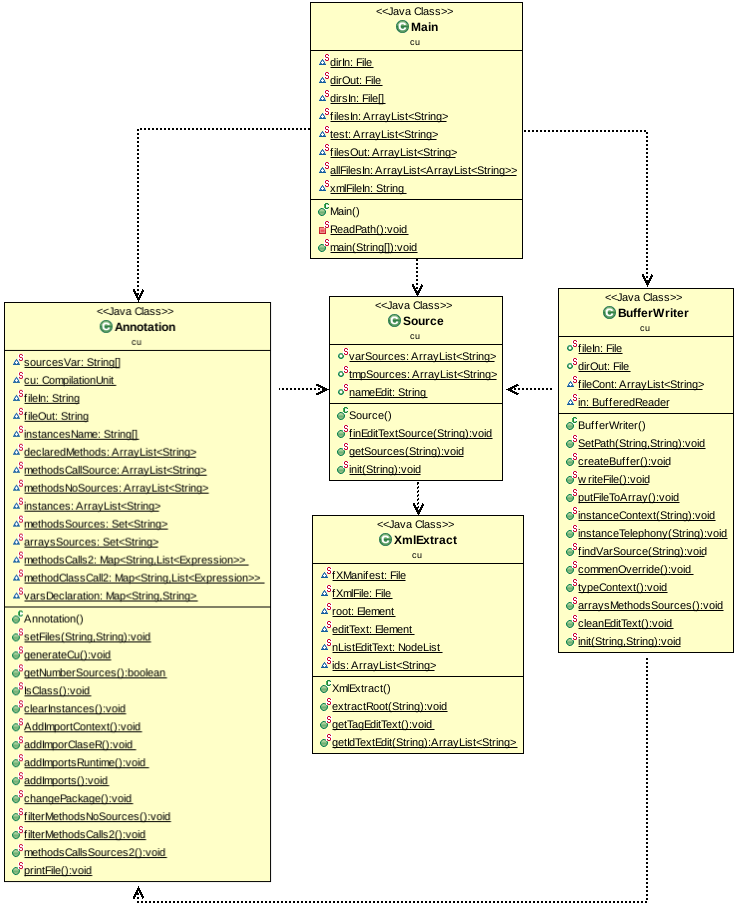
\includegraphics[width=13cm]{consolidado.png}
	\caption{Clases necesarias para la implementación del anotador}
	\label{fig:classDiagram} 
\end{figure}

\section{Descripción de testcases para evaluación}
\label{tb:muestra-descripApps}
\label{sec:testcases}
En las tablas \ref{tab:descripApps1}, \ref{tab:descripApps2} y
\ref{tab:descripApps3}, se describe el comportamiento de los casos de prueba
evaluados, donde:\newline 
Se considera con nivel de seguridad alto, variables y métodos que almacenan y
modifican(respectivamente), información catalogada como privada(Sources).\newline 
Se considera con nivel de seguridad bajo, métodos para envío de mensajes y para
muestra de logs.

En los casos en que se requiere, se precisan observaciones entre los
resultados de evaluación esperados para la técnica de análisis utilizada por
FlowDroid y la técnica de análisis propuesta en el presente trabajo.

\begin{table}[H]
\small\addtolength{\tabcolsep}{-3pt}
\caption{Descripción aplicaciones de prueba}
\label{tab:descripApps1}
\begin{tabular}{|p{13cm}|p{1cm}|}
	\hline
	\multicolumn{2}{|>{\columncolor[gray]{0.8}}c|}{\textbf{AndroidSpecific\_DirectLeak1}}\\
	\hline
	\textbf{Descripción} & \textbf{Leaks}\\
	\hline
	La variable \textit{mrg} tiene un nivel de seguridad alto,
	almacena información retornada por el método source \textit{getDeviceId}. Se
	genera flujo de información directo entre información con nivel de seguridad alto e
	información con nivel de seguridad bajo, al enviar como parámetro del método
	\textit{sendTextMessage}, información de la variable \textit{mrg}. & 1 \\
	\hline
	\multicolumn{2}{|>{\columncolor[gray]{0.8}}c|}{\textbf{AndroidSpecific\_InactiveActivity}}\\
	\hline
	\textbf{Descripción} & \textbf{Leaks}\\
	\hline 
	La variable \textit{imei} tiene un nivel de seguridad alto, almacena
	información retornada por el source getDeviceId. La variable es enviada como
	parámetro a \textit{Log}, canal que muestra información con nivel de
	seguridad bajo. \textit{Observación:} debido a que la actividad en que se
	presenta este flujo de información no está activada en el Manifest de la
	aplicación, para la técnica de análisis de FlowDroid no existen leaks. Para
	nuestra propuesta de análisis si existe leak, porque se asume que los métodos y
	sus aplicaciones podrán ser ejecutados. & 0
	\\
	\hline
	\multicolumn{2}{|>{\columncolor[gray]{0.8}}c|}{\textbf{AndroidSpecific\_LogNoLeak}}\\
	\hline
	\textbf{Descripción} & \textbf{Leaks}\\
	\hline
	El caso de prueba no presenta información con niveles de seguridad alto. Se
	presentan flujos de información entre información con el mismo nivel de
	seguridad, en este caso bajo, lo cual es permitido. & 0 \\
	\hline
	\multicolumn{2}{|>{\columncolor[gray]{0.8}}c|}{\textbf{AndroidSpecific\_Obfuscation1}}\\
	\hline
	\textbf{Descripción} & \textbf{Leaks}\\
	\hline 
	La variable \textit{\textbf{mrg}} tiene un nivel de seguridad alto,
	almacena información retornada por el método source getDeviceId().
	Se genera flujo de información entre información con nivel de seguridad alto e
	información con nivel de seguridad bajo, al enviar como parámetro del método
	\textit{sendTextMessage}, información de la variable
	\textit{mrg}. \textit{Observación:} el elemento adicional para este
	testcase es proveer una suplantación de la clase
	android.telephony.TelephonyManager, en el apk de la aplicación. Para la
	evaluación que proponemos, se verifica acorde a la versión que se tiene anotada
	para esta clase, es decir, independientemente de la ofuscación de la clase,
	nuestro análisis debe detectar que existe un flujo de información indebido. &
	1\\
	\hline
	\multicolumn{2}{|>{\columncolor[gray]{0.8}}c|}{\textbf{AndroidSpecific\_PrivateDataLeak2}}\\
	\hline
	\textbf{Descripción} & \textbf{Leaks}\\
	\hline
	La variable \textit{info} tiene un nivel de seguridad alto, almacena
	información suministrada por el campo EditText de tipo textPassword. Se genera
	flujo de información entre información con nivel de seguridad alto e
	información con nivel de seguridad bajo, al pasar la variable
	\textit{info} como parámetro de \textit{Log}, que muestra
	información con nivel de seguridad bajo. & 1 
	\\
	\hline
	\multicolumn{2}{|>{\columncolor[gray]{0.8}}c|}{\textbf{ArraysAndLists\_ArrayAccess1}}\\
	\hline
	\textbf{Descripción} & \textbf{Leaks}\\
	\hline
	Se tiene un array en que se almacena información tanto proveniente como no
	proveniente de sources, parte de la información que almacena es enviada como
	parámetro del método \textit{sendTextMessage}. \textit{Observación:}
	Para la técnica de análisis de FlowDroid(taint analysis), se marca únicamente el
	índice del array donde se almacena el dato considerado como source, así,
	cuando se envía como parámetro del método \textit{sendTextMessage},
	el dato de un índice no marcado, no se genera leak. Para nuestra técnica
	de análisis(flujo de información mediante JIF), para que un array almacene
	información con nivel de seguridad alto, primero debe ser catalogo(anotado)
	con nivel de seguridad alto, lo que implica que el array podrá almacenar
	información tanto de nivel de seguridad alto como bajo, pero toda la
	información quedará con nivel de seguridad alto. En consecuencia, al enviar
	cualquier índice del array como parámetro del método 
	\textit{sendTextMessage} se presenta un flujo de información no
	permitido. & 0
	\\
	\hline
\end{tabular}
\end{table}

\begin{table}[H]
\small\addtolength{\tabcolsep}{-3pt}
\caption{Descripción aplicaciones de prueba}
\label{tab:descripApps2}
\begin{tabular}{|p{13cm}|p{1cm}|}
	\hline
	\multicolumn{2}{|>{\columncolor[gray]{0.8}}c|}{\textbf{ArraysAndLists\_ArrayAccess2}}\\
	\hline
	\textbf{Descripción} & \textbf{Leaks}\\
	\hline
	Se presenta el contexto descrito en ArraysAndLists\_ArrayAccess1, con un
	elemento adicional, se implementa el método calculateIndex(), que calcula el
	índice del array a ser enviado como parámetro del método
	\textit{sendTextMessage}. & 0 \\
	\hline
	\multicolumn{2}{|>{\columncolor[gray]{0.8}}c|}{\textbf{GeneralJava\_Exceptions1}}\\
	\hline
	\textbf{Descripción} & \textbf{Leaks}\\
	\hline
	La variable \textit{imei} es de nivel de seguridad alto, almacena información
	devuelta por el método \textit{getDeviceId}. Se genera flujo de información
	entre información de nivel de seguridad alto e información con nivel de
	seguridad bajo, al enviar como parámetro del método \textit{sendTextMessage}
	información de la variable \textit{imei}. Este flujo de información se presenta
	dentro de la captura de una excepción RuntimeException(no es verificada
	en tiempo de compilación).
	& 1
	\\
	\hline
	\multicolumn{2}{|>{\columncolor[gray]{0.8}}c|}{\textbf{GeneralJava\_Exceptions2}}\\
	\hline
	\textbf{Descripción} & \textbf{Leaks}\\
	\hline
	La variable \textit{imei} es de nivel de seguridad alto, almacena información
	devuelta por el método \textit{getDeviceId}. El control de flujo del
	programa conduce de manera implícita a la captura de una excepción tipo
	RuntimeException, desde allí se utiliza información proveída por la variable
	\textit{imei}, como parámetro para invocar el método \textit{sendTextMessage}.
	Generando un flujo de información indebido. & 1
	\\
	\hline
	\multicolumn{2}{|>{\columncolor[gray]{0.8}}c|}{\textbf{GeneralJava\_Exceptions3}}\\
	\hline
	\textbf{Descripción} & \textbf{Leaks}\\
	\hline
	La variable \textit{imei} es de nivel de seguridad alto, almacena información
	devuelta por el método \textit{getDeviceId}. La información proveída por
	\textit{imei} es utilizada como parámetro para invocar el método
	\textit{sendTextMessage} dentro de la captura de una excepción tipo
	RuntimeException, sin embargo, el programa no genera un caso que haga ejecutar
	la captura de la excepción. & 0
	\\
	\hline
	\multicolumn{2}{|>{\columncolor[gray]{0.8}}c|}{\textbf{GeneralJava\_Exceptions4}}\\
	\hline
	\textbf{Descripción} & \textbf{Leaks}\\
	\hline
	La variable \textit{imei} es de nivel de seguridad alto, almacena información
	devuelta por el método \textit{getDeviceId}. información proveída por esta
	variable es enviada como parámetro para la captura de una excepción en tiempo
	de ejecución, donde es utilizado como parámetro para invocar el método
	\textit{sendTextMessage}, generando un flujo de información indebido. & 1\\
	\hline
	\multicolumn{2}{|>{\columncolor[gray]{0.8}}c|}{\textbf{GeneralJava\_Loop1}}\\
	\hline
	\textbf{Descripción} & \textbf{Leaks}\\
	\hline
	La variable \textit{imei} es de nivel de seguridad alto, almacena información
	devuelta por el método \textit{getDeviceId}. Se generan flujos de información
	indebidos, primero al tratar de asignar la información de la variable a un
	array con nivel de seguridad bajo(donde se intenta ofuscar la información),
	luego al tratar de enviar la información ofuscada como parámetro del método
	\textit{sendTextMessage}, con nivel de seguridad bajo. & 1 \\
	\hline
	\multicolumn{2}{|>{\columncolor[gray]{0.8}}c|}{\textbf{GeneralJava\_Loop2}}\\
	\hline
	\textbf{Descripción} & \textbf{Leaks}\\
	\hline
	La variable \textit{imei} es de nivel de seguridad alto, almacena información
	devuelta por el método \textit{getDeviceId}. Se busca ofuscar la información de
	\textit{imei} mediante ciclos for anidados, allí se asigna la información de la
	variable a un array con nivel de seguridad bajo. Luego se envía la información
	ofuscada, como parámetro del método \textit{sendTextMessage}, con nivel de
	seguridad bajo, generando otro flujo de información indebido. & 1\\
	\hline
\end{tabular}
\end{table}

\begin{table}[H]
\small\addtolength{\tabcolsep}{-3pt}
\caption{Descripción aplicaciones de prueba}
\label{tab:descripApps3}
\begin{tabular}{|p{13cm}|p{1cm}|}
	\multicolumn{2}{|>{\columncolor[gray]{0.8}}c|}{\textbf{GeneralJava\_UnreachableCode}}\\
	\hline
	\textbf{Descripción} & \textbf{Leaks}\\
	\hline
	La variable \textit{deviceid} con nivel de seguridad alto, está contenida en un
	método que no es llamado, dentro del mismo, \textit{deviceid} es pasada como
	parámetro para invocar el método \textit{sendTextMessage}, cuyo nivel de
	seguridad es bajo. \textit{Observaciones:} para el análisis de FlowDroid el
	programa no presenta leaks, ya que el método nunca es llamado.
	Para nuestro análisis, el programa presenta leak porque se asume que todos los
	métodos son llamados. & 0\\
	\hline
	\multicolumn{2}{|>{\columncolor[gray]{0.8}}c|}{\textbf{ImplicitFlows\_ImplicitFlow1}}\\
	\hline
	\textbf{Descripción} & \textbf{Leaks}\\
	\hline
	 La variable \textit{imei} con nivel de seguridad alto, almacena información
	 devuelta por el método \textit{getDeviceId}, \textit{imei} se pasa como
	 parámetro al método obfuscateIMEI que devuelve la información ofuscada.
	 Después se invoca el método WriteToLog, con la información ofuscada como
	 parámetro para ser mostrada en el log. Al invocar el método WriteToLog con la
	 información ofuscada, se genera un flujo de información indebido. & 1 \\
	\hline
	\multicolumn{2}{|>{\columncolor[gray]{0.8}}c|}{\textbf{ImplicitFlows\_ImplicitFlow2}}\\
	\hline
	\textbf{Descripción} & \textbf{Leaks}\\
	\hline
	 La variable \textit{userInputPassword} con nivel de seguridad alto, almacena
	 información de un campo EditText tipo textPassword(password suministrado por
	 el usuario). Se generan flujos de información indebidos: al tratar de asignar
	 información a la variable passwordCorrect con nivel de seguridad bajo, a
	 partir de la comparación de información con nivel de seguridad alto(variable
	 textPassword), después, al tratar de mostrar en el \textit{log} información
	 que depende de tal comparación. & 1\\
	\hline
	\multicolumn{2}{|>{\columncolor[gray]{0.8}}c|}{\textbf{ImplicitFlows\_ImplicitFlow4}}\\
	\hline
	\textbf{Descripción} & \textbf{Leaks}\\
	\hline
	La variable \textit{password} con nivel de seguridad alto, almacena información
	de un campo EditText tipo textPassword, \textit{password} es utilizada como
	parte de los parámetros para invocar el método \textit{lookup} que busca
	identificar el password suministrado por el usuario. Se genera un flujo de
	información indebido, cuando se compara lo retornado por el método para mostrar
	en el \textit{log} información del password. & 1 \\
	\hline
	\multicolumn{2}{|>{\columncolor[gray]{0.8}}c|}{\textbf{Lifecycle\_ActivityLifecycle3}}\\
	\hline
	\textbf{Descripción} & \textbf{Leaks}\\
	\hline
	 El flujo de información entre información con nivel de seguridad alto e
	 información con nivel de seguridad bajo, tiene lugar a través de dos
	 métodos del ciclo de vida de la actividad: onSaveInstanceState y
	 onRestoreInstanceState. En onSaveInstanceState, se asigna información con
	 nivel de seguridad alto a la variable \textit{s}, la información que almacene
	 este método es utilizada durante la reanudación de la actividad, a través del
	 método onRestoreInstanceState, donde se muestra en el \textit{log} información
	 de la variable \textit{s}. & 1\\
	\hline
	\multicolumn{2}{|>{\columncolor[gray]{0.8}}c|}{\textbf{Lifecycle\_BroadcastReceiverLifecycle1}}\\
	\hline
	\textbf{Descripción} & \textbf{Leaks}\\
	\hline
	 Se tiene un broadcast receiver  que muestra información con nivel de
	 seguridad alto, contenida en la variable \textit{imei}(almacena información retornada por el
	 método \textit{getDeviceId}) a través del \textit{log}. & 1 \\
	\hline
	\multicolumn{2}{|>{\columncolor[gray]{0.8}}c|}{\textbf{Lifecycle\_ServiceLifecycle1}}\\
	\hline
	\textbf{Descripción} & \textbf{Leaks}\\
	\hline
	 Se tiene un servicio que presenta flujo de información indebida mediante dos
	 métodos de su ciclo de vida. En el método que inicia el servicio
	 onStartCommand, la variable con nivel de seguridad alto, almacena
	 información devuelta por el método \textit{getDeviceId}. Luego el método
	 onLowMemory, se envía información de la variable \textit{secret} a través de
	 un mensaje msm. & 1\\
	\hline
\end{tabular}
\end{table}

% \section{Formulas}
% Las formulas \ref{p} y \ref{r} son aplicadas para calcular los porcentajes
% de Precisión(p) y Recall(r).
% \begin{equation}
% \label{p}
% 	p = TP/(TP +FP) 
% \end{equation}
% \begin{equation}
% \label{r}
% 	r = TP/(TP+FN)
% \end{equation}
% 
% Donde: \newline
% TP representa el total de verdaderos positivos; FP corresponde al total de
% falsos positivos y  FN representa el total de falsos
% negativos; reportados por la herramienta.\newline

\section{Instrucciones para probar el prototipo}
\label{sec:ejecutarPrototipo}
En el directorio \small{\ttfamily{/home/testing/eule}} están los elementos
necesarios para evaluar los casos de prueba, de allí interesan los
subdirectorios \small{\ttfamily{androidFlows}},
\small{\ttfamily{InputLabelGenerator}} y el jar
\small{\ttfamily{LabelGenerator.jar}}.

El subdirectorio \small{\ttfamily{androidFlows}} contiene la estructura de
archivos necesaria para ejecutar un programa jif, así:
\small{\ttfamily{sig-src}} aloja clases java y clases de la API de Android, con
signaturas para que jif las reconozca de forma nativa.
\small{\ttfamily{jif-src/test}} tiene clases de la API de Android con
anotaciones jif(Activity.jif, BroadcastReceiver.jif, Log.jif, R.jif,
Service.jif, SmsManager.jif). Allí se deben alojar los programas jif a
ejecutar.\newline 
En {\small{\ttfamily{InputLabelGenerator}}} están los fuentes java a pasar como
entrada para el generador de labels(LabelGenerator.jar), que devuelve la
versión jif de los mismos. Se recomienda utilizar estos, ya que contienen las
adaptaciones necesarias para poder ser analizadas con JIF, la adición de
excepciones NullPointerException, ClassCastException y
ArrayIndexOutOfBoundsException, son algunos ejemplos de elementos adicionados.

 \textbf{Instrucciones de
ejecución:}\newline \textbf{(1)} Ejecutar el jar para la generación de los labels:
\begin{lstlisting}
testing@debianJessie:~/eule$ java -jar LabelGenerator.jar
\end{lstlisting}
Una vez se ejecuta el .jar, se solicita el directorio de entrada(que contiene
las aplicaciones a anotar) y el directorio de salida(para alojar las
aplicaciones anotadas). Separados por el simbolo @
\begin{lstlisting}
Ingrese la ruta completa para el directorio de entrada, y para el 
directorio de salida:
Ejemplo: dir-entrada@dir-salida 
\end{lstlisting}
Se deben pasar los directorios:
\begin{lstlisting}
InputLabelGenerator@androidFlows/jif-src/test/
\end{lstlisting}

\textbf{(2)} ejecutar el script setup.sh(basta con ejecutarlo una sola vez)
\begin{lstlisting}
testing@debianJessie:~/eule/androidFlows$ ./setup.sh
\end{lstlisting}

\textbf{(3)} 
Ejecutar el .jif generado:\newline
En la ruta pasada como directorio de salida en el punto anterior
{\small{\ttfamily{androidFlows/jif-src/test}}}, se genera un subdirectorio por
aplicación, con un .java y un *-out.jif. Se debe ejecutar el *-out.jif. Por
ejemplo, para evaluar el testcase ArraysAndLists\_ArrayAccess1:
\begin{lstlisting}
testing@debianJessie:~/eule/androidFlows$ ./jifc-java-libraries.sh \
jif-src/test/ArraysAndLists_ArrayAccess1/ArrayAccess1-out.jif
\end{lstlisting}
Cuando se presentan flujos indebidos, el compilador genera una salida señalando
los problemas de seguridad.
\lstset{
    language=bash,
    basicstyle=\tiny,
  }
\begin{lstlisting}
estudiante@debianJessie:~/eule/androidFlows$ ./jifc-java-libraries.sh \
jif-src/test/ArraysAndLists_ArrayAccess1/ArrayAccess1-out.jif 
/home/testing/eule/androidFlows/jif-src/test/ArraysAndLists_ArrayAccess1/ArrayAccess1-out.jif:51:
Unsatisfiable constraint
    	general constraint:
    		actual_arg_3 <= formal_arg_3
    	in this context:
    		{Alice->; _<-_ ⊔ caller_pc} <= {}
    	cannot satisfy equation:
    		{Alice->} ⊑ {}
    	in environment:
    		{this} ⊑ {caller_pc}
    		[]

    Label Descriptions
    ------------------
     - actual_arg_3 = the label of the 3rd actual argument
     - actual_arg_3 = {Alice->; _<-_ ⊔ caller_pc}
     - formal_arg_3 = the upper bound of the formal argument text
     - formal_arg_3 = {}
     - caller_pc = The pc at the call site of this method (bounded above by 
    {})
     - this = label of the special variable "this" in test.ArrayAccess1

    The label of the actual argument, actual_arg_3, is more restrictive than 
    the label of the formal argument, formal_arg_3.
            sms.sendTextMessage("+49 1234", null, arrayData[2], null, null);
                                                  ^-------^

1 error.
testing@debianJessie:~/eule/androidFlows$
\end{lstlisting}

Cuando el caso de prueba no presenta flujos indebidos, el compilador no genera
salidas, por ejemplo, al evaluar el testcase AndroidSpecific\_LogNoLeak, el
compilador retorna el prompt de la shell, sin ningún comentario.

\section{Instrucciones para uso de FlowDroid}
En el directorio \small{\ttfamily{/home/estudiante/eule}} también se encuentran
los subdirectorios \small{\ttfamily{/FlowDroid}} y
\small{\ttfamily{/DroidBench-master}} que contienen los elementos necesarios
para probar los testcases con FlowDroid.\newline 
Para ello se requiere ejecutar el jar de FlowDroid, indicando el apk a analizar,
los apk están en el subdirectorio \tetxtit{DroidBench-master}.
Por ejemplo, para analizar el testace ImplicitFlow4:
\begin{lstlisting}
testing@debianJessie:~/eule/FlowDroid$ java -jar FlowDroid.jar \
../DroidBench-master/apk/ImplicitFlows/ImplicitFlow4.apk
/home/estudiante/android-sdks/platforms/
\end{lstlisting}
El archivo \small{\ttfamily{howRunIt}} contenido en el directorio
\small{\ttfamily{/FlowDroid}}, indica como se debe ejecutar.
 \bibliographystyle{IEEEtran} 
 \bibliography{referencias}
  
\end{document}